\PassOptionsToPackage{table, dvipsnames}{xcolor}
\documentclass[a4paper,twoside,12pt]{vendor/toptesi}
\usepackage[T1]{fontenc}
\usepackage[utf8]{inputenc}
\usepackage[italian]{babel}
\usepackage{graphicx}
\usepackage{tikz}
\usepackage{float}
\usetikzlibrary{positioning}
\usepackage{pgfplots}
\usepackage[newfloat,outputdir=build]{minted}
\usepackage[font=small,skip=1pt]{caption}
\captionsetup[listing]{position=top}
\usepackage{subcaption}
\usepackage{xspace}
\usepackage{fontawesome5}
\usepackage{minted}
\pgfplotsset{compat=1.18}

\SetupFloatingEnvironment{listing}{name=Codice}

\usepackage{hyperref}

\hypersetup{
    colorlinks = true,
    allcolors=black
}

\hyphenation{di-spo-si-ti-vi}

%%% workaround for listing
% save the current meaning of \listing
\let\savedlisting\listing
% at the right spot, restore the meaning
\AtBeginDocument{\let\listing\savedlisting}
%%% end of workaround


\def\dept{Dipartimento di Ingegneria Elettrica e dell’Informazione}
\def\course{Corso di Laurea triennale in Ingegneria Informatica e dell’Automazione}
\def\title{DIFESA DI SISTEMI INFORMATIVI TRAMITE FIREWALL IN COMPETIZIONI ATTACCO/DIFESA}
\def\author{Domingo Dirutigliano}
\def\prof{Chiar.mo Prof.\ Gennaro Boggia}
\def\supervisor{Dott.Ing. Daniele Pugliese}
\def\subject{RETI DI TELECOMUNICAZIONI}
\def\annoacc{2024\ -\ 2025}
\def\beforecandidate{Laureando}
\def\beforetitle{Tesi di Laurea in}
\def\beforeprof{Relatore}
\def\beforesupervisor{Correlatore}
\def\beforeannoacc{Anno Accademico}

\makeatletter
\def\cleardoublepage{\clearpage\if@twoside\ifodd\c@page\else
    \hbox{}
    \vspace*{\fill}
    \vspace{\fill}
    \thispagestyle{empty}
    \newpage
    \if@twocolumn\hbox{}\newpage\fi\fi\fi}
\makeatother

\makeatletter
\renewcommand{\@makefntext}[1]{%
  \scriptsize
  \parindent1em%
  \noindent\hb@xt@1.8em{\@makefnmark\hss}#1%
}
\makeatother


\begin{document}

%\maketitle


\begin{titlepage}
	\begin{tikzpicture}[remember picture,overlay]
		\centering
			\node[yshift=-6 cm] (logo) at (current page.north) {\includegraphics[width=0.35\linewidth]{images/poliba.png}};
			\node[text width=50em,yshift=0.25cm, align = center, below = of logo](poliba){\bfseries \Large POLITECNICO DI BARI};
			\node[text width=40em, align = center, yshift=.55cm,below = of poliba](course){\normalsize \dept \\
% 
				\normalsize \textbf{\course}};
		\node[text width=35em,align = center,  yshift=1.2cm,below = of course](line){\par\noindent\rule{\textwidth}{0.4pt}};
		\node[text width=40em, align = center, yshift=.60cm,below = of line](beftitle){\beforetitle};
		\node[text width=40em, align = center, yshift=.95cm,below = of beftitle](lia){\subject};
		\node[text width=40em, align = center, yshift=-0.5cm,below = of lia](title){\bfseries \fontsize{21pt}{20pt}\selectfont \hyphenpenalty=10000 \exhyphenpenalty=10000 \title\par};
	\node[text width=35em, align = left, yshift=-1.70cm,below = of title](prof){\large \beforeprof \\ \textbf{\prof}};
	\node[text width=35em, align = left, yshift=0.4cm,below = of prof](supervisor){\large \beforesupervisor \\ \textbf{\supervisor}};
		\node[text width=35em, align = right, yshift=0cm,below = of supervisor](candidate){\large \beforecandidate\\ \textbf{\author}};
		\node[text width=35em,align = center,  yshift= 0cm,below = of candidate](line2){\par\noindent\rule{\textwidth}{0.4pt}};
		\node[text width=50em, align = center, yshift=0.5cm,below = of line2](year){\beforeannoacc\xspace \annoacc};
	\end{tikzpicture}
\end{titlepage}


% \cleardoublepage
% % Dedication

\thispagestyle{empty}
%\refstepcounter{dummy}

\pdfbookmark[1]{Dedication}{Dedication} % Bookmark name visible in a PDF viewer

\vspace*{3cm}

%\begin{center}
%\emph{Ohana} means family. \\
%Family means nobody gets left behind, or forgotten. \\ \medskip
%--- Lilo \& Stitch    
%\end{center}

\medskip

\begin{flushright}
\textit{Dedication, \\ continuing dedication.} \\ \smallskip
%%1939\,--\,2005
\end{flushright}

% \cleardoublepage

\pagenumbering{roman}

\chapter*{Abstract}

L'aumento esponenziale di attacchi cyber, fenomeni di data breach e violazioni della privacy ha elevato la cybersecurity a priorità strategica a livello globale, determinando una crescente domanda di professionisti specializzati, capaci di fronteggiare scenari dinamici attraverso competenze tecniche multidisciplinari e approcci innovativi.
Tra le metodologie di addestramento delle nuove generazioni di esperti spicca la gamification applicata alle competizioni \gls{ctf}. Queste sfide simulano scenari reali, fornendo un laboratorio pratico per acquisire competenze tecniche in contesti operativi, sviluppare capacità di problem solving under pressure e comprendere le dinamiche degli attacchi moderni.
Inoltre, esistono competizioni organizzate in tutto il mondo che riuniscono e si rivelano sfidanti per la comunità di hacker e professionisti della sicurezza informatica, spesso promosse direttamente da grandi aziende.
In questo quadro si inserisce il presente lavoro, finalizzato alla progettazione e sviluppo di un modulo di un firewall specializzato per \gls{ctf} di tipologia \gls{ad}. La soluzione proposta integra funzionalità avanzate di analisi del traffico in \textit{real-time} e meccanismi adattivi di filtraggio, permettendo di scrivere filtri direttamente in linguaggio Python.
Il modulo si dimostra altamente configurabile e versatile, caratteristiche essenziali per questo tipo di competizioni. L'architettura è stata progettata al fine di garantire un elevato throughput nonostante l’uso di un linguaggio interpretato, grazie all'uso di tecniche di parallelizzazione e all'implementazione eseguita in linguaggio C++.


\cleardoublepage
\tableofcontents
\cleardoublepage

\newcommand{\footcite}[2]{\footnote{#1\hspace{\fill}\cite{#2}}}

\pagenumbering{arabic}
\setcounter{page}{1}
\chapter*{Introduzione}\label{chap:intro}
\addcontentsline{toc}{chapter}{Introduzione}
\pagenumbering{arabic}
\setcounter{page}{1}

L'era digitale, caratterizzata da una connettività globale senza precedenti, ha portato con sé una crescente esposizione a minacce informatiche sofisticate. Attacchi ransomware, violazioni di dati sensibili, phishing avanzato e exploit zero-day rappresentano oggi una realtà quotidiana, con impatti devastanti su infrastrutture critiche, istituzioni finanziarie e diritti individuali. Secondo il Global Risk Report 2025 del World Economic Forum\footcite{Global Risks Report 2025: \url{https://www.weforum.org/publications/global-risks-report-2025/}}{weforumGRR2025}, la cybersecurity si colloca tra i primi cinque rischi globali in termini di probabilità e gravità, sottolineando l'urgente necessità di rafforzare la resilienza dei sistemi e formare professionisti in grado di anticipare, contenere e neutralizzare queste minacce.

In questo contesto, la domanda di esperti con competenze tecniche multidisciplinari: dalla crittografia all'analisi forense, dalla sicurezza di rete alla psicologia degli attaccanti, ha superato l'offerta creando un divario che richiede approcci innovativi alla formazione.

Le tradizionali metodologie didattiche, spesso teoriche e frammentate, si rivelano insufficienti per preparare figure capaci di operare in scenari dinamici, dove la rapidità decisionale e la creatività strategica sono determinanti.

Un ruolo chiave in questa transizione formativa è svolto dalle competizioni \gls{ctf}, che combinano gamification e simulazione di scenari reali per offrire un addestramento immersivo. Queste sfide, strutturate in categorie come jeopardy, \gls{ad} o Boot-to-Root, ricreano ambienti controllati in cui i partecipanti devono identificare vulnerabilità, sfruttare exploit, difendere servizi e analizzare tracce malevole. Non solo favoriscono l'acquisizione di competenze tecniche, ma allenano il problem solving under pressure, la collaborazione in team e la capacità di adattamento a tattiche in continua evoluzione. Eventi internazionali come il Google \gls{ctf}\footcite{\url{https://capturetheflag.withgoogle.com/}}{google_ctf}, patrocinato da aziende leader del settore, attirano migliaia di partecipanti, trasformandosi in vetrine per il reclutamento di talenti e laboratori per testare strumenti all'avanguardia.

L'obiettivo in queste competizioni è rubare la flag: una stringa di testo segreta, con un formato ben riconoscibile, ottenibile sfruttando vulnerabilità volutamente esposte nei sistemi. La flag rappresenta pertanto la prova univoca che attesta la risoluzione della sfida da parte dei partecipanti. Queste competizioni costituiscono un ottimo strumento per approfondire le proprie competenze nel settore anche per i più esperti, che spesso ricoprono sia il ruolo di giocatori che di organizzatori in diverse competizioni, alimentando un ciclo virtuoso di apprendimento, innovazione e crescita collettiva all'interno dell'ecosistema cybersecurity\footcite{\url{https://www.hackthebox.com/blog/what-is-ctf/}}{hackthebox_ctf}.

Particolare rilevanza assumono le competizioni di tipo \gls{ad}, in cui i team devono simultaneamente proteggere i propri sistemi dagli avversari e compromettere quelli altrui. Questa modalità richiede una comprensione profonda delle dinamiche offensive e difensive, oltre alla capacità di implementare contromisure in tempo reale.

Questa tesi tratta la progettazione e lo sviluppo di un firewall orientato alle competizioni \gls{ctf} di tipologia \gls{ad}, le quali richiedono tool flessibili in grado di adattarsi dinamicamente alle varie fasi della competizione. Verranno analizzate le funzionalità attualmente presenti nel progetto, i punti critici e le possibili migliorie per aumentarne l'efficienza e le prestazioni. In particolare, l'attenzione si concentrerà su una nuova funzionalità sviluppata che consente l'applicazione di filtri in modo totalmente trasparente dal punto di vista dell'applicativo, che mira a minimizzare l'impatto sulla rete, e permette di definire le regole di filtraggio utilizzando istruzioni in linguaggio Python.

Il firewall oggetto di questa tesi è Firegex\footcite{\url{https://github.com/Pwnzer0tt1/firegex}}{firegex_gh}, sviluppato per il team del Politecnico di Bari\footcite{\url{https://www.poliba.it}}{poliba_website} in occasione della competizione nazionale di Cyberchallenge\footcite{\url{https://cyberchallenge.it/}}{cyberchallenge} del 2022. In tale contesto è nato lo stesso team \gls{ctf} che ne ha supportato lo sviluppo, Pwnzer0tt1\footcite{\url{https://pwnzer0tt1.it/}}{pwnzer0tt1}.

La nuova funzionalità implementata, denominata \gls{nfproxy}, simula il funzionamento di un proxy tradizionale per il filtraggio del traffico. Il suo funzionamento e caratteristiche tecniche saranno oggetto del Capitolo~\ref{chap:nfproxy}.

La struttura del documento è organizzata come segue. Nel Capitolo~\ref{chap:ctfad} verranno forniti i dettagli relativi alle competizioni \gls{ctf} \gls{ad}, descrivendo l'infrastruttura tipica di gara, il funzionamento dei componenti principali e gli strumenti comunemente utilizzati dai partecipanti.

Il Capitolo~\ref{chap:firegex} presenterà Firegex analizzandone le motivazioni alla base dello sviluppo, il confronto con soluzioni esistenti, l'architettura interna e le principali funzionalità offerte.

Il Capitolo~\ref{chap:nfproxy} si focalizzerà sulla progettazione e sviluppo del modulo nfproxy, approfondendo le scelte architetturali, le problematiche nell'elaborazione parallela dei pacchetti e le soluzioni implementate per la gestione del traffico \gls{tcp} e \gls{http}.

Il Capitolo~\ref{chap:tests} descriverà la metodologia adottata per i test di funzionalità e performance, inclusi i benchmark comparativi e i risultati ottenuti.

Infine, il Capitolo~\ref{chap:notes} conterrà considerazioni finali su possibili sviluppi futuri ed in particolare una vulnerabilità emersa durante il progetto nel kernel linux.


\afterpage{\blankpage}
\chapter{Competizioni CTF Attack/Defense}\label{chap:ctfad}
\setcounter{page}{5}

Le competizioni \gls{ctf} di tipo \gls{ad} sono una tipologia di competizioni in cui i partecipanti devono difendere i propri servizi e attaccare i servizi degli avversari, in un contesto di gara estremamente dinamico e competitivo.

In queste competizioni prendono parte diversi team, i quali vengono associati ognuno ad una macchina, solitamente linux, con in esecuzione un insieme di servizi ogniuno dei quali presenta vulnerabilità\footcite{\url{https://faustctf.net/information/attackdefense-for-beginners/}}{faustctf_attackdefense_for_beginners}.

I servizi sono accessibili tramite la rete di gara, e sono replicati su tutte le macchine.

\section{Descrizione dell'infrastruttura}

L'infrastruttura di una competizione CTF Attack/Defense è composta da diversi componenti chiave che interagiscono in modo sinergico.

Possiamo individuare tre elementi principali che costituiscono l'infrastruttura di gara:
\begin{itemize}
    \setlength{\itemsep}{2pt}
    \setlength{\parskip}{2pt}
    \item Il \textbf{Gameserver}, cuore centrale del sistema che gestisce la competizione
    \item I \textbf{Checker}, responsabili del monitoraggio continuo della rete e dei servizi
    \item Le \textbf{VM dei team}, che ospitano i servizi vulnerabili
\end{itemize}

Il funzionamento di ogniuno di questi componenti è approfondito nei paragrafi successivi, evidenziando inoltre tutte le peculiarità e le funzionalità utili allo svolgimento della competizione.

\subsection{Il Gameserver e i Checker}

Al centro di tutta la competizione c'è il gameserver, entità (che può essere composta da uno o più host) che prende in carico la gestione della competizione eseguento una serie di azioni e fornendo diversi servizi descritti in questo capitolo, essenziali per lo svolgimento della gara stessa.

La competizione è strutturata in tick (o round), ovvero intervalli di tempo in cui ciclicamente il gameserver assegna punti ai team in base alle azioni compiute dagli stessi, e monitora i servizi tramite i checker.

Questo tempo può variare da competizione a competizione. I checker sono dei bot che si occupano di supervisionare lo stato della gara eseguendo diverse azioni come:

\begin{itemize}
    \setlength{\itemsep}{2pt}
    \setlength{\parskip}{2pt}
    \item Verificare se il servizio è funzionante e raggiungibile, andando a connettersi ed eseguendo azioni di normale utilizzo, assicurandone anche l'integrità.

    \item Utilizzare il servizio per memorizzare al suo interno una flag, inserita come informazione sensibile normalmente non accessibile seguendo i normali workflow del servizio.

    \item Verificare che le flag inserite nei tick precedenti siano ancora raggiungibili tramite un normale accesso autorizzato, e che pertanto non siano state modificate o rimosse dal team possessore di quella macchina.
\end{itemize}

In generale, rimuovere vecchie flag, avere il servizio non raggiungibile e non avere la possibilità di inserirne di nuove, sono azioni che vanno ad invalidare la normale attività del servizio: il gameserver, rilevate queste problematiche, lo andrà a considerare come totalmente o parzialmente inaccessibile o manomesso, in base alle scelte degli organizzatori.

Si evidenzia come i checker non sfruttino mai le vulnerabilità dei servizi, ma si limitino al loro corretto utilizzo.

\subsection{I servizi, le flag e i flag store}

Ogni flag viene generata e inserita dai checker nel servizio dei vari team ad ogni tick, con una flag sempre differente dalle altre ed ha usualmente una durata massima di valenza (e.g, 5 tick): in questo intervallo di tempo è ancora possibile rubare e consegnare la flag al gameserver ottenendo punti.

Le flag infatti una volta ottenute vanno consegnate al gameserver, che tramite un calcolo che può variare in diverse competizioni, assegna punti al team che l'ha consegnata.

\begin{listing}[H]
\begin{minted}[
    frame=single,
    framerule=0.8pt,
    fontsize=\footnotesize,
    breaklines
]{python}
scale = 15 * sqrt(5) 
norm = ln(ln(5)) / 12 
offense_points[flag] = scale / (1+exp((sqrt(score[attacker][service]) - sqrt(score[victim][service]))*norm))
defense_points[flag] = min(victim_score, offense_points)
\end{minted}
\caption{Algoritmo di calcolo del valore della flag in CyberChallenge\footciteref{cyberchallenge_ad_rules}}\label{lst:flagcalc}
\end{listing}

Il defense point è il punteggio sottratto al team da cui è stata rubata la flag come parte del punteggio di difesa descritto successivamente.

All'interno della competizione spesso possono esserci dei team di `prova' chiamati \gls{nop} team: questi sono semplicemente macchine non associate a nessun gruppo reale di persone, che offrono i servizi della gara, al solo scopo di renderli usufruibili per eseguire penetration testing. Il loro utilizzo è particolarmente utile ai partecipanti per provare gli attacchi in maniera quanto più fedele e realistica possibile, eseguendo l'attacco su una replica originale del servizio, e non su una potenzialmente soggetta alle modifiche e alle patch del team avversario. Non tutte le competizioni prevedono la presenza dei \gls{nop} team.

Si noti che consegnare le flag del proprio team o quelle appartenenti ai \gls{nop} team non permette di guadagnare nessun punteggio, e ciò è possibile poichè il gameserver ha traccia di tutte le flag, di chi le consegna, e delle macchine in cui sono state originariamente inserite.

Una caratteristica importante da sottolineare riguardo ai servizi di cui si è parlato fino ad ora è che non è sempre vero che per ognuno di essi ci sia una sola flag per tick ed una sola vulnerabilità per singolo tick. Infatti, ogni servizio ha usualmente multiple vulnerabilità e flag per tick al suo interno: i checker che si occupano di inserire le flag potrebbero inserirne diverse, usando diverse parti o impostazioni del servizio.

In caso di servizi con più flag, diremo che questi conterranno diversi flag store. Ciò detto fino ad ora è pertanto valido per ogni flag store, e non per il servizio in generale.

Si noti infine che esiste un set di checker differente per ogni flag store.

\subsection{I Flag ID}

Il gameserver potrebbe rilasciare delle informazioni aggiuntive per ogni flag store, come ad esempio un username, che di per se non va direttamente a permettere l'accesso protetto alla flag, ma da un informazione utile agli attaccanti al fine di poterla individuare più facilmente all'interno del servizio stesso.

Questa informazione aggiuntiva è chiamata Flag ID e viene rilasciata per ogni team, per ogni flag store, e per ogni flag ancora valida nel momento in cui si visita l'\gls{api} esposta dal gameserver, che le espone pubblicamente per tutti i partecipanti. Non è possibile manomettere i Flag ID, in quanto sono informazioni direttamente rilasciate dagli organizzatori, che comunque in assenza di vulnerabilità nei servizi, risultano insufficienti per ottenere flag.

\subsection{Calcolo del punteggio}

A ciascun flag store in gara viene associato un punteggio, che riflette la capacità del team di sfruttare e proteggere le relative vulnerabilità. Il calcolo del punteggio totale si ottiene tradizionalmente mediante una semplice sommatoria dei punteggi parziali.

Il punteggio attribuito a un singolo store è inizialmente determinato da un valore base, soggetto a variazioni durante la competizione in relazione alle prestazioni del team.

Tale valore può essere incrementato o ridotto in base a tre componenti aggiuntive:

\begin{itemize}
    \setlength{\itemsep}{2pt}
    \setlength{\parskip}{2pt}
    \item \textbf{Punteggio di \gls{sla}}: misura la disponibilità del servizio, calcolata in proporzione al tempo di effettiva operatività.
    Questo indicatore, generalmente in percentuale, viene applicato al punteggio complessivo dello store. La scelta di attribuirgli un ruolo predominante mira a scoraggiare strategicamente la disattivazione volontaria dei servizi per evitare attacchi, penalizzando severamente tale approccio. Di conseguenza, il mantenimento dell'operatività del servizio (pur nella sua condizione vulnerabile) assume un'importanza critica nella competizione.

    \item \textbf{Punteggio di attacco}: determinato dal numero di invii corretti di flag effettuati dal team. Il valore attribuito a ciascuna flag può variare in funzione della complessità dell'attacco e della tempestività con cui il servizio è stato compromesso rispetto agli altri team.

    \item \textbf{Punteggio di difesa}: tipicamente negativo, poiché quantifica l'inefficacia delle contromisure, è calcolato in base al numero di flag sottratte al team da parte degli avversari. Tale componente tende a controbilanciare, o persino ridurre, il punteggio di attacco relativo allo stesso flag store, potendolo portare anche al di sotto del valore base iniziale. La sua entità è modulata da criteri analoghi a quelli usati per il punteggio di attacco. Per mitigarne gli effetti, risulta essenziale applicare interventi correttivi (\emph{patch}) che impediscano nuovi attacchi, garantendo al contempo la piena operatività del servizio e l'integrità dei dati archiviati (comprese le flag precedenti, la cui perdita comporterebbe un deterioramento del punteggio di \gls{sla}).
\end{itemize}

\begin{figure}[H]
    \centering
    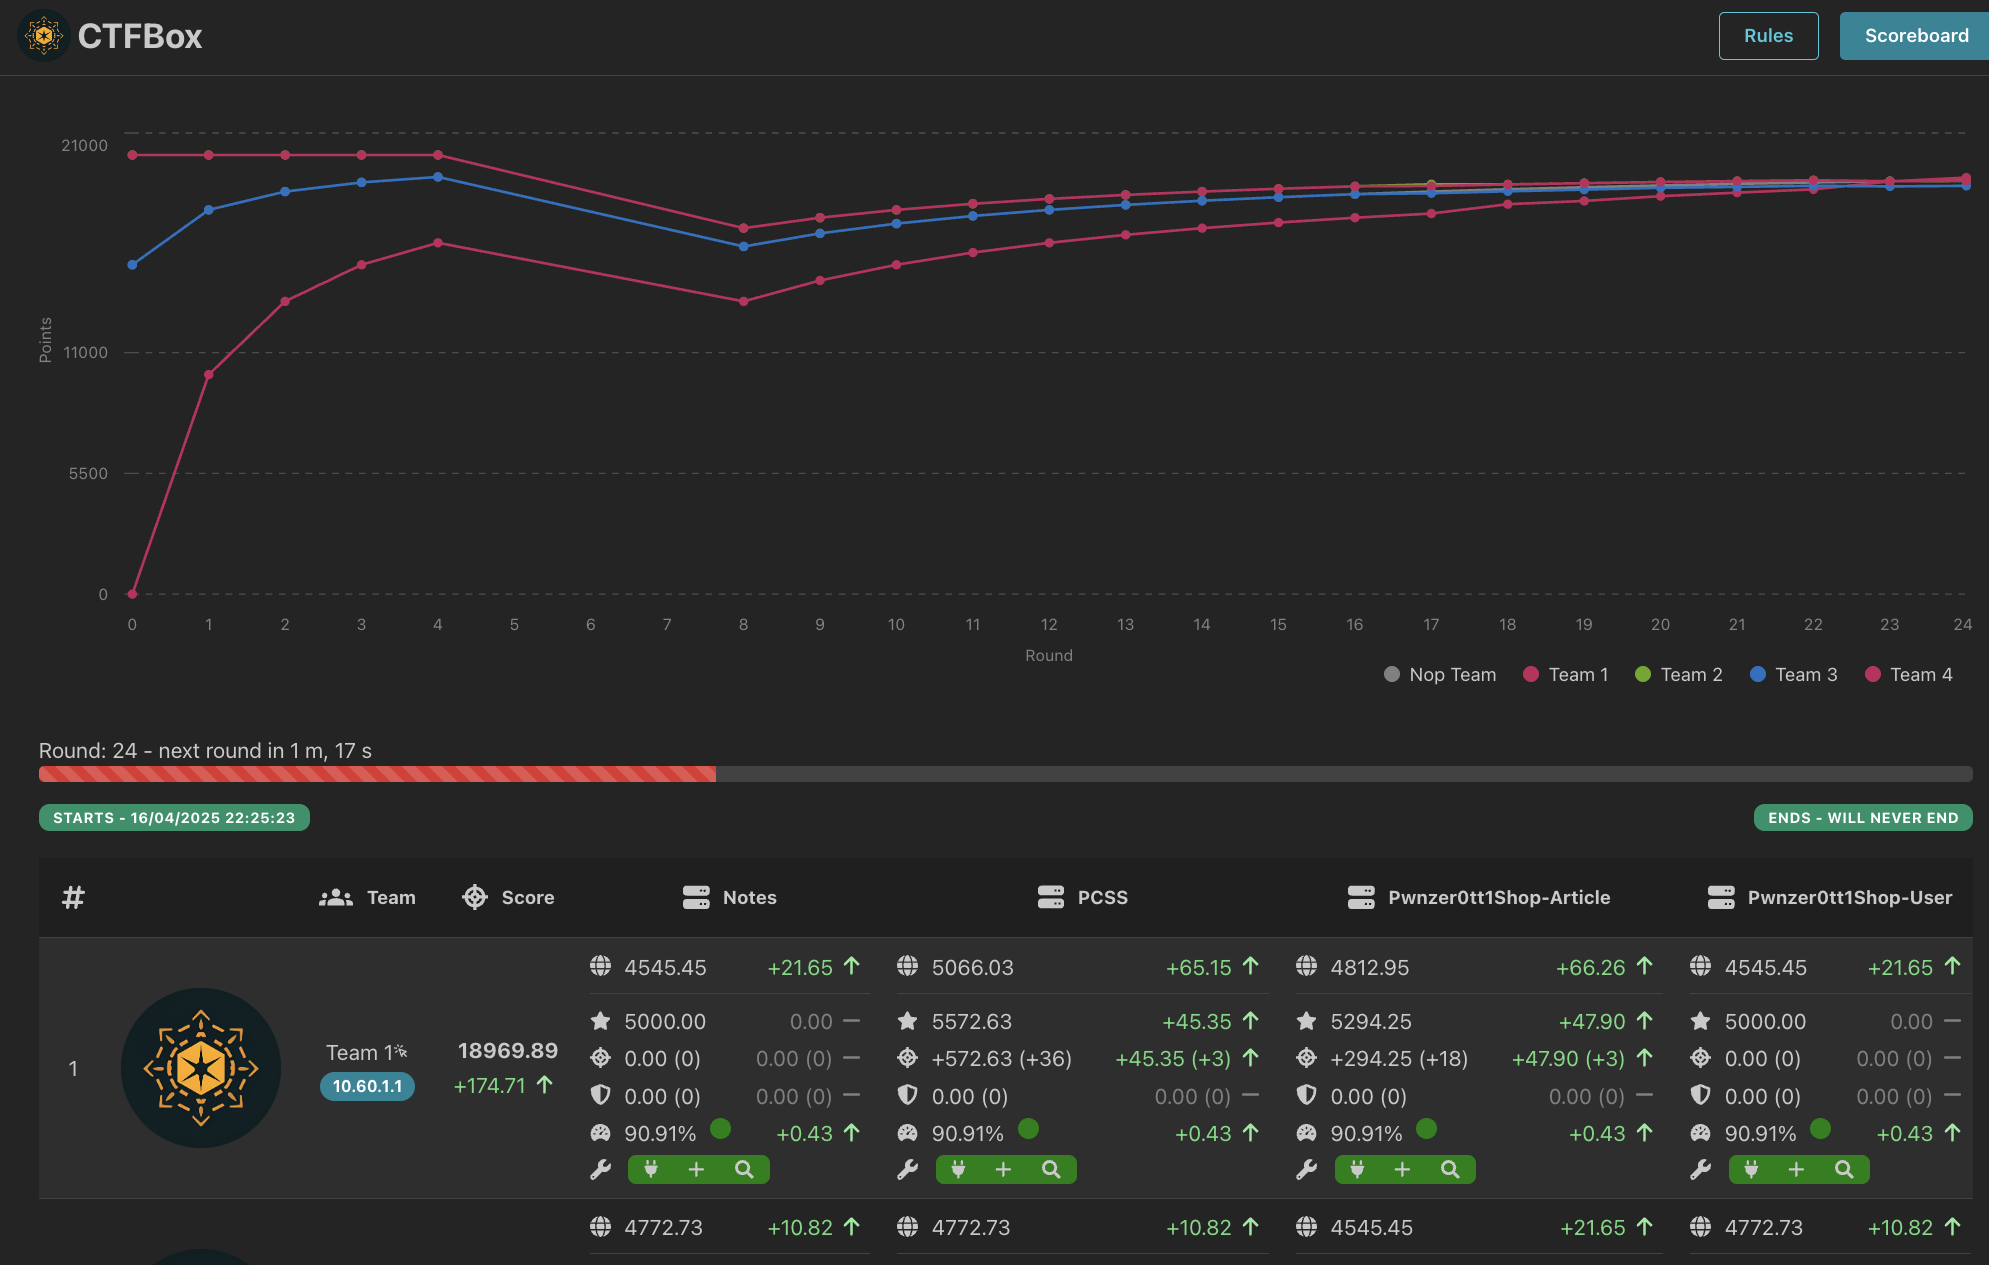
\includegraphics[width=0.98\textwidth]{images/chapter1/ctfbox_scoreboard.png}
    \caption{Scoreboard di una simulazione realizzata con CTFBox\footciteref{ctfbox_gh}}\label{fig:ctfbox_scoreboard}
\end{figure}

\begin{listing}[H] 
\begin{minted}[
    frame=single,
    framerule=0.8pt,
    fontsize=\footnotesize,
    breaklines
]{python}
# --- Total score for each service (or better said, flag store) ---

# Service base points 
score[team][service] = 5000 
            
# Sum offensive points 
for flag in stolen_flags[team][service]:
    score[team][service] += offense_points[flag] 
    
# Substract defensive points 
for flag in lost_flags[team][service]: 
    score[team][service] -= defense_points[flag]

# --- Final team score ---

total_score[team] = 0 
        
for service in services: 
    # Compute SLA of the service
    sla[team][service] = ticks_up[team][service] / ticks[team][service] 
    # Limit scores to 0
    score[team][service] = max(0, score[team][service]) 
    # Add service score
    total_score[team] += score[team][service] * sla[team][service]

\end{minted}
\caption{Algoritmo di calcolo del punteggio in CyberChallenge\footciteref{cyberchallenge_ad_rules}}\label{lst:scorecalc}
\end{listing}

\vspace{\fill}
\newpage

\subsection{Rete di gara}

Per questa analisi si prende in considerazione la rete di gara in utilizzo per le competizioni nazionali di Cyberchallenge\footcite{\url{https://ad.cyberchallenge.it/rules/}}{cyberchallenge_ad_rules}, sottolineando come a grandi linee la configurazione di rete è spesso simile, ma potrebbe variare in base alle competizioni e agli organizzatori.

\begin{figure}[H]
    \centering
    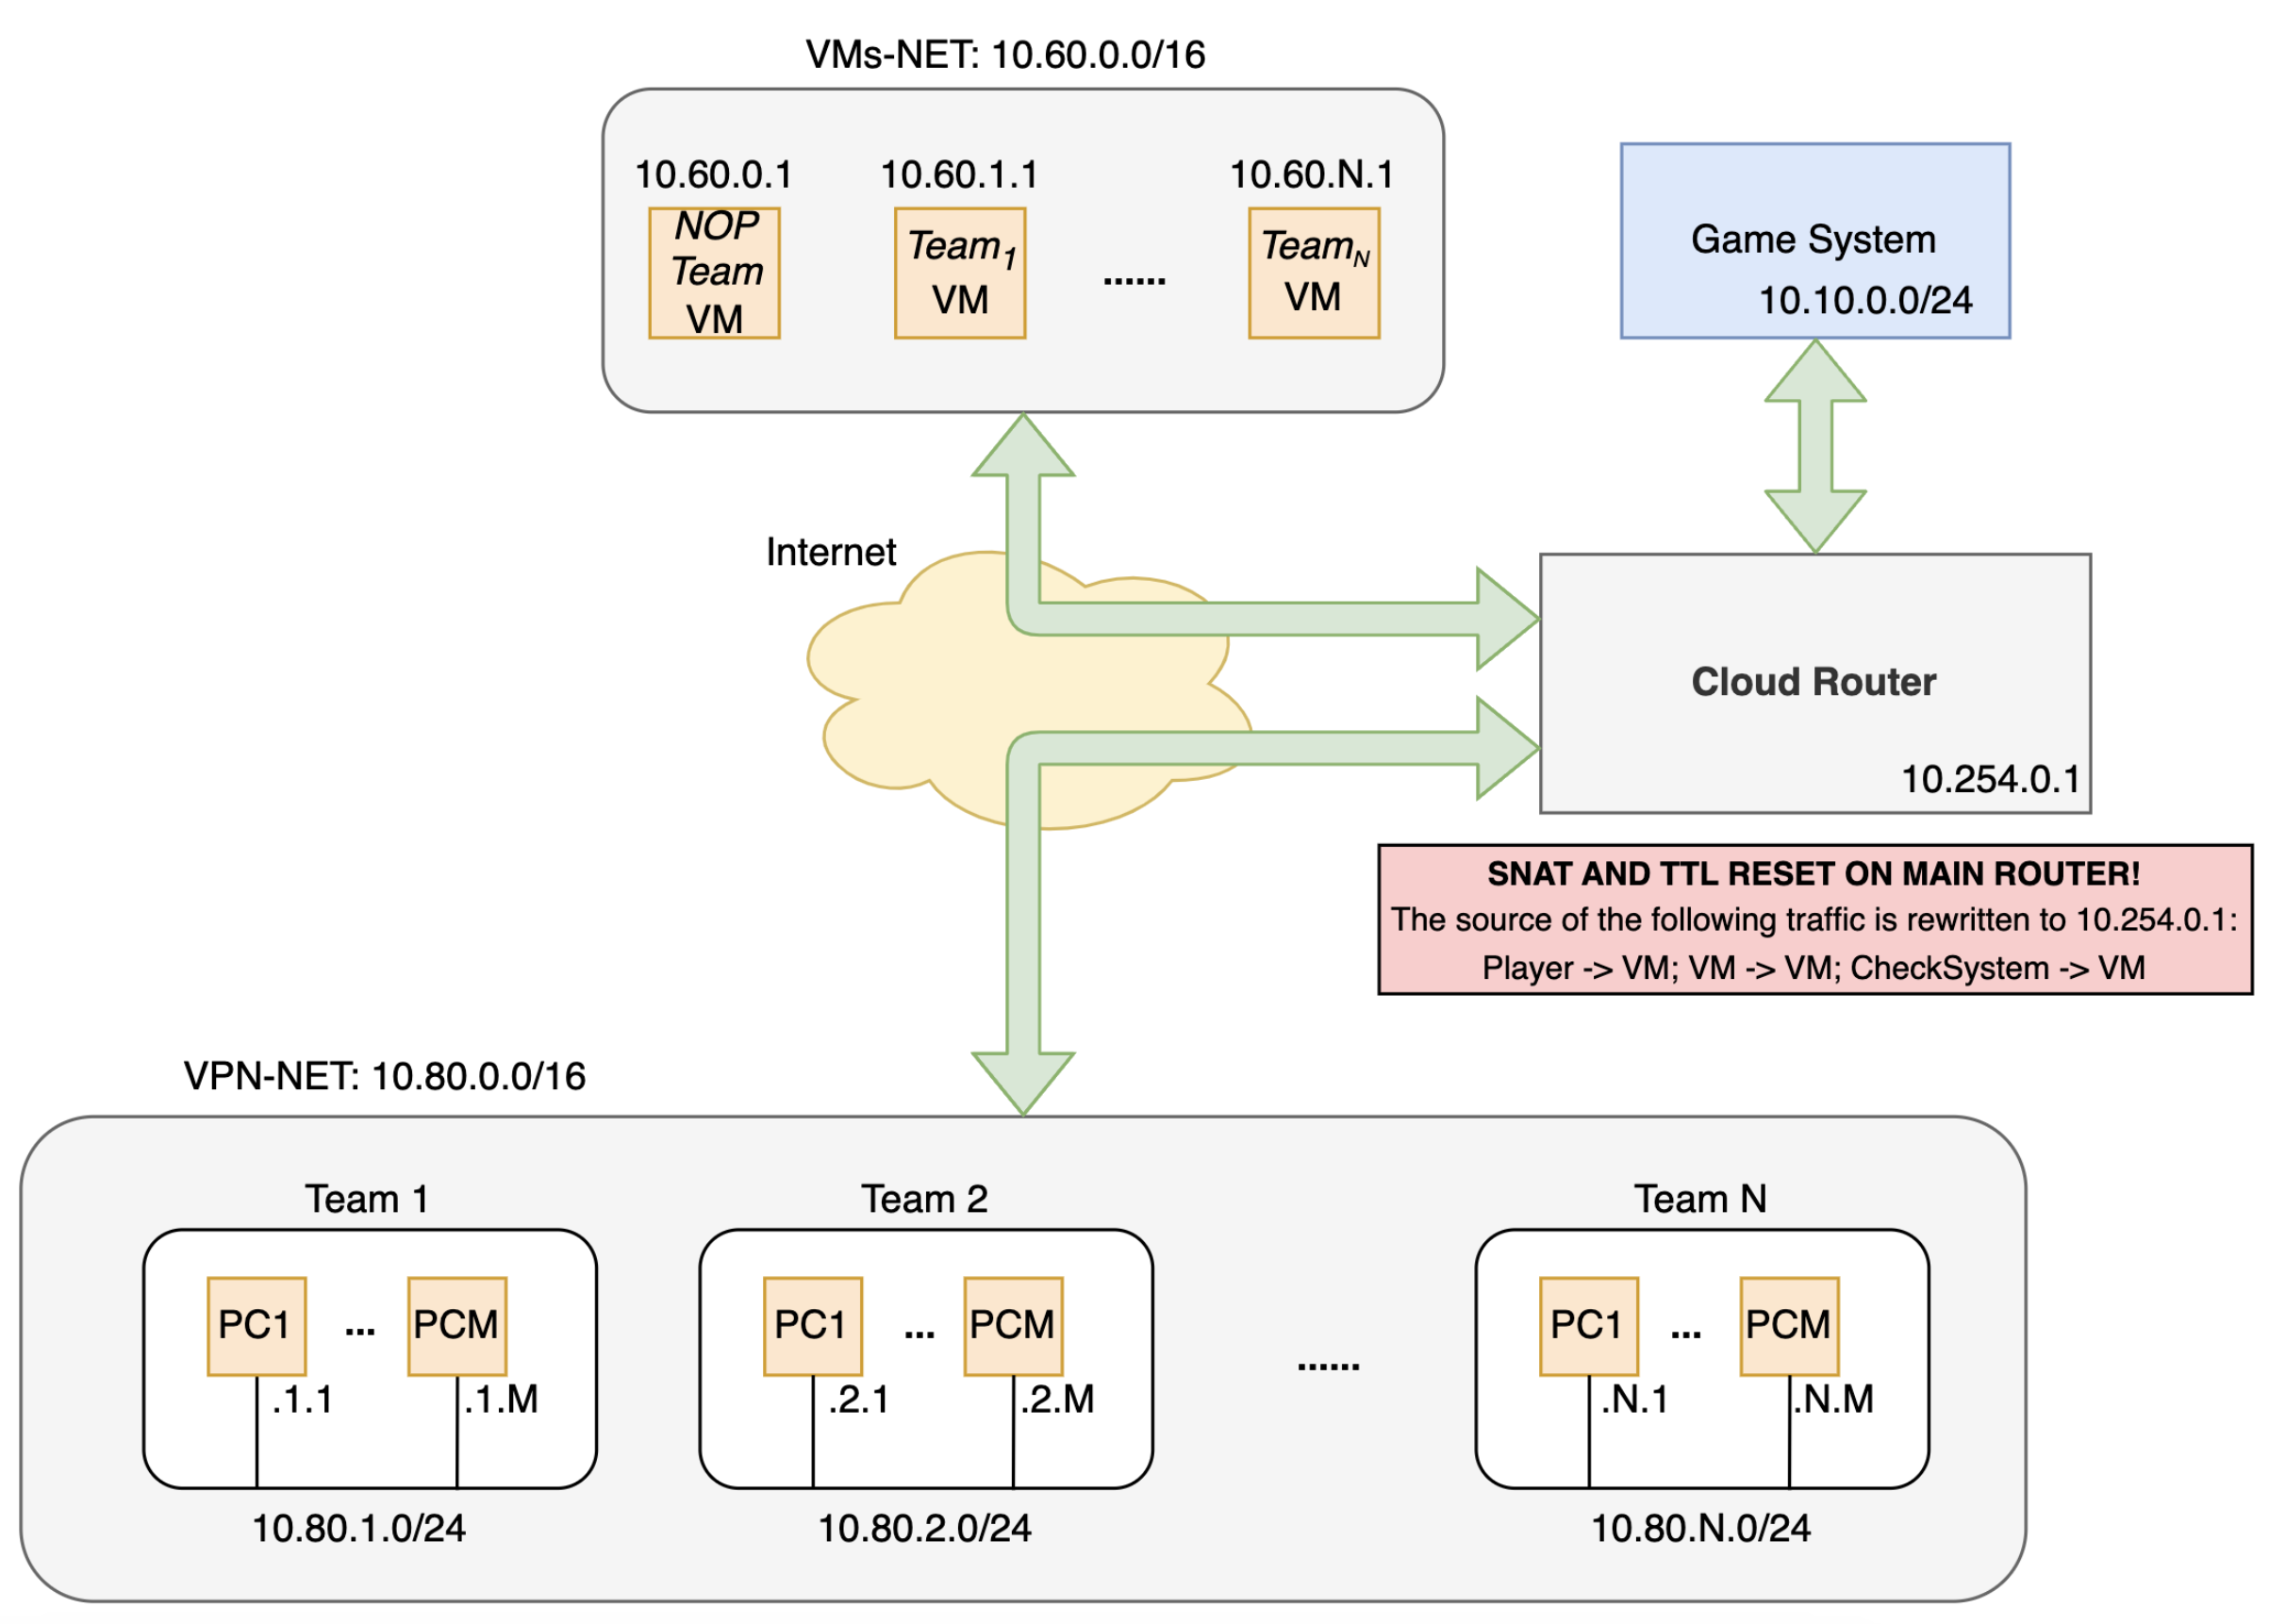
\includegraphics[width=0.8\textwidth]{images/chapter1/ccit_network.png}
    \caption{Modello della rete di gara di Cyberchallenge\footciteref{cyberchallenge_ad_rules}}\label{fig:ccit_network}
\end{figure}

Come si può vedere nella Figura~\ref{fig:ccit_network}, la rete di gara è composta da diversi elementi:
\begin{itemize}
    \setlength{\itemsep}{2pt}
    \setlength{\parskip}{2pt}
    \item La rete dedicata agli organizzatori, dove abbiamo il gameserver (potenzialmente formato da un insieme di host) ed eventuali ulteriori host al servizio degli organizzatori.

    \item La sottorete delle macchine dei team, dove si ha accesso ssh alla propria macchina con i propri servizi vulnerabili.

    \item Una sottorete (spesso realizzata tramite \gls{vpn}) per ogni team, dove sono connessi gli host dei partecipanti con i quali è possibile interagire direttamente con la rete di gara.
\end{itemize}

Al centro di tutto ciò troviamo il cloud router, che si occupa di gestire il traffico in base alle regole imposte dagli organizzatori e in base alla fase in cui si trova la competizione, ma che soprattutto si occupa di anonimizzare il traffico, manipolandolo tramite diverse tecniche tra le quali il \gls{nat}. Tramite il \gls{nat} infatti si nascondono gli indirizzi \gls{ip} delle macchine e dei componenti del team, mascherando nelle richieste la vera identità del mittente con quella del router stesso. Questo è un elemento di fondamentale importanza poichè altrimenti sarebbe davvero molto semplice diversificare le connessioni dei checker da quelle degli attaccanti, andando a perdere l'obiettivo che ha la competizione stessa, ovvero: individuare, sfruttare e difendersi dalle vulnerabilità.

Inoltre si specifica che le reti dei singoli team sono isolate per tutta la competizione al fine di evitare possibili attacchi agli host dei partecipanti, che non sono dei target di interesse nella gara e per cui non è consentita l'esecuzione di attacchi mirati.
Un simile comportamento potrebbe portare alla squalifica del team attaccante a seguito di segnalazioni e analisi del traffico da parte degli organizzatori.

\section{Svolgimento della competizione}

Una competizione \gls{ad} inizia nel momento in cui viene dato accesso alle macchine e alla rete di gara. Usualmente in questa fase c'è un periodo di tempo in cui la rete rimane non accessibile: i team avranno accesso unicamente alle loro macchine, mentre l'accesso ai servizi degli avversari verrà negato. In questo momento tuttavia è già possibile analizzare i servizi, avviare tutti i tool necessari all'avvio degli attacchi, all'analisi della rete, e alla difesa del server (che analizzeremo nel prossimo paragrafo). Finito questo periodo di tempo, la rete di gara viene aperta, e la competizione inizia ufficialmente.

Da ora il gameserver inizia a scandire i tick, i checker iniziano ad utilizzare i servizi e ad inserire le prime flag, pubblicando anche i primi Flag ID.
I team iniziano a lavorare, tentando di difendersi dai primi attacchi, e a loro volta di attaccare rubando le prime flag agli avversari, tutto ciò mantenendo sempre i loro servizi attivi e funzionanti. Ad ogni tick, il gameserver assegna i nuovi punteggi, e i team possono osservare tramite questi dati l'evoluzione della gara stessa, comprendendo quali possono essere le azioni da compiere per massimizzare la crescita del loro punteggio.
Inoltre, viene segnalato pubblicamente quali dei servizi di quale team non sono funzionanti, e perchè sono considerati down: cioè la motivazione per cui i checker hanno segnalato un mal funzionamento.
La competizione termina ad un determinato orario di fine, dove la rete di gara viene chiusa, e il gameserver interrompe l'azione dei checker non accettando, inoltre, nuove submission di flag.

Tutto quello descritto in questo capitolo è possibile simularlo e sperimentarlo tramite il progetto CTFBox\footcite{\url{https://github.com/domysh/ctfbox}}{ctfbox_gh}, nato come fork di Oasis dei TheRomanXpl0it\footcite{\url{https://theromanxpl0.it/about.html}}{theromanxploit} con cui è possibile simulare ma anche svolgere competizioni \gls{ad} di medio-piccole dimensioni in un ambiente realizzato unicamente tramite l'utilizzo di container, con funzionamento e regolamento simile a quello di CyberChallenge\footcite{\url{https://ad.cyberchallenge.it/rules/}}{cyberchallenge_ad_rules}.

\section{Tool utili}

Data l'elevata complessità nello svolgimento di una competizione \gls{ad}, spesso diventa necessario l'utilizzo di tool specializzati che permettano di automatizzare diverse operazioni necessarie durante la gara. Ogni team può sviluppare e utilizare anche tool che facilitano (o perfino che automatizzino) l'attacco e la difesa dei servizi.

In generale i tool utilizzati più frequentemente sono quelli descritti di seguito.

\subsection{Traffic Analyzer}

I tool di analisi del traffico permettono di investigare il flusso di dati sulla macchina, in modo da riconoscere e visionare il traffico dei checker e degli attaccanti (anche se anonimizzato). Analizzare il traffico diventa cruciale dal momento in cui un nuovo attacco è attivo sulla rete, poichè permette ai team di analizzarlo, riconoscere la vulnerabilità sfruttata, e intraprendere azioni quanto più immediate per la difesa e la replicazione dello stesso attacco. Normalmente per analizzare il traffico è possibile usare tool tradizionali quali Wireshark\footcite{\url{https://www.wireshark.org/}}{wireshark} o Suricata\footcite{\url{https://suricata.io/}}{suricata}, che tuttavia risultano poco pratici nel loro utilizzo in ambito \gls{ctf} \gls{ad} dove il traffico da analizzare è elevato e continuo. Esistono infatti, tool scritti appositamente per queste competizioni che permettono di analizzarlo in modo più efficiente e veloce, ma anche di riprodurre velocemente gli stessi payload di attacco, come ad esempio Caronte\footcite{\url{https://github.com/eciavatta/caronte}}{caronte} o Tulip\footcite{\url{https://github.com/OpenAttackDefenseTools/tulip}}{tulip}.

Ad esempio Caronte\footciteref{caronte} avvantaggia particolarmente l'analisi del traffico grazie alla sua interfaccia grafica interattiva e di facile utilizzo, che permette di visualizzare i flussi di traffico \gls{tcp} aggregati e decodificati in pochissimi click, e permettendone anche il tagging tramite l'utilizzo di \gls{regex} personalizzate, che permettono ad esempio di identificare una flag in uscita (quindi rubata o controllata dal checker) e le flag in entrata (quindi le nuove flag inserite dal gameserver). Ogni connessione è classificata tramite tag e colori personalizzabili in base alla porta di destinazione (e.g.\ \gls{http}:\ blu, SSH:\ verde), permettendo una mappatura visiva immediata dei servizi sotto attacco. Inoltre include una timeline interattiva, campionata al minuto per scorrere la porzione di traffico che si desidera analizzare.

\begin{figure}[H]
    \centering
    
\includegraphics[width=0.20\textwidth]{images/chapter1/CaronteLogo.png}
    \caption{Logo di caronte}\label{fig:caronte_logo}
\end{figure}

\begin{figure}[H]
    \centering
    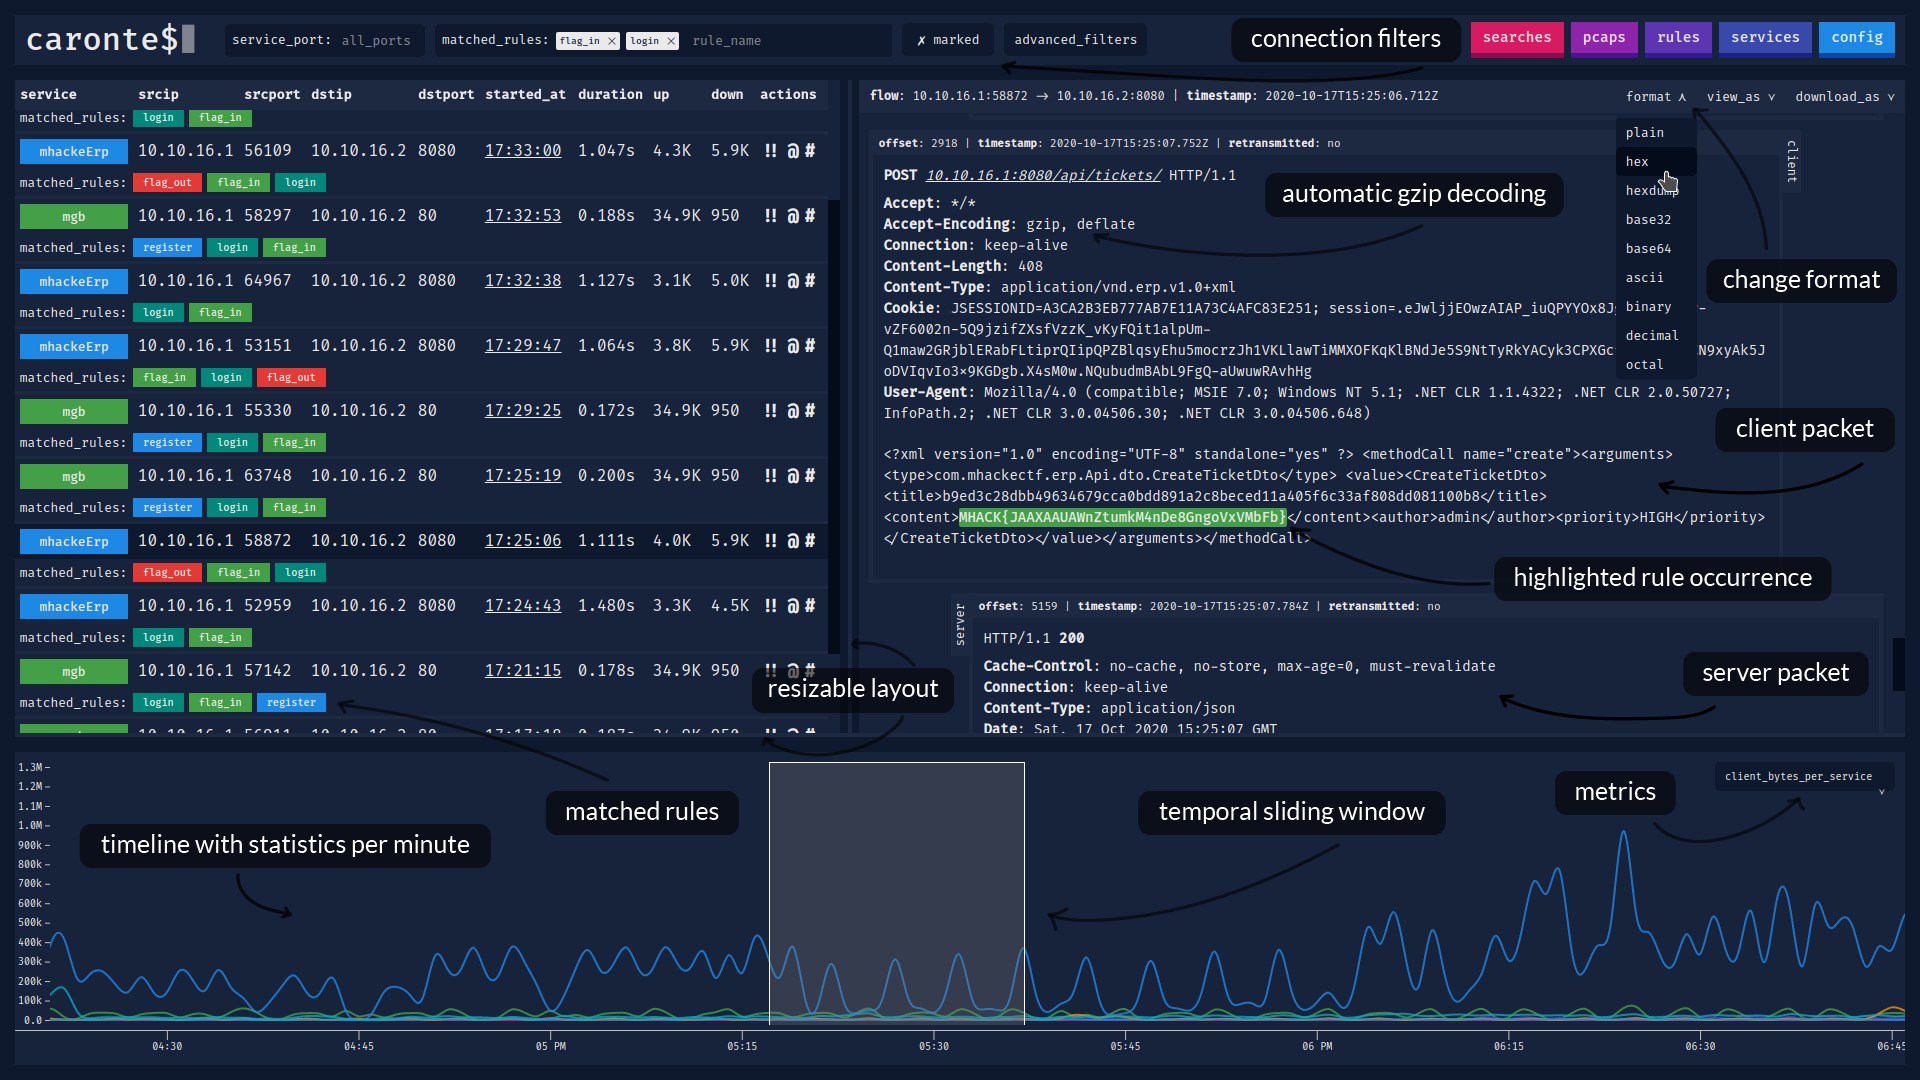
\includegraphics[width=0.98\textwidth]{images/chapter1/caronte_interface.png}
    \caption{Interfaccia di Caronte}\label{fig:caronte_interface}
\end{figure}

\subsection{Attacker \& Submitter}

Gli strumenti di attacco e submission automatizzati coordinano gli attacchi, assistono nella scrittura degli exploit e ne monitorano l'esecuzione, programmandola e parallelizzandola. Questi tool sono fondamentali per permettere all'attaccante di concentrarsi sulla progettazione del singolo attacco, anziché sulla gestione della sua esecuzione su tutte le macchine nemiche. Inoltre, grazie alla tracciabilità degli attacchi, è possibile identificare problemi durante l'esecuzione e monitorare quali team iniziano a difendere i propri servizi. Solitamente (ma non sempre) questi strumenti gestiscono anche la submission delle flag al gameserver in modo centralizzato, semplificando il rispetto delle regole organizzative che limitano frequenza e quantità per prevenire attacchi bruteforce o DoS all'infrastruttura.

Esempi di tali tool includono DestructiveFarm\footciteref{destructivefarm}, che presenta tuttavia criticità nell'analisi dell'andamento degli attacchi, e ExploitFarm\footciteref{exploitfarm}, sviluppato proprio per ovviare a queste limitazioni. A differenza di DestructiveFarm\footciteref{destructivefarm}, ExploitFarm\footciteref{exploitfarm} offre un coordinamento più efficiente degli attacchi, un monitoraggio avanzato e una schedulazione semplificata, supportando attacchi distribuiti su più macchine con funzionalità di analisi in tempo reale.

La sua infrastruttura ricalca quella di DestructiveFarm\footciteref{destructivefarm}: un server centrale gestisce gli exploit e le submission, mentre client distribuiti eseguono gli attacchi e inviano le flag al server, bilanciando il carico computazionale derivante dalla replicazione degli exploit. Il sistema include un client terminale per l'esecuzione degli attacchi e un'interfaccia web centralizzata per il monitoraggio e l'analisi. La piattaforma è orientata alla raccolta dati e alla reportistica, con funzionalità di versioning degli exploit, registrazione dettagliata di ogni esecuzione e analisi delle cause di fallimento per ottimizzare gli attacchi.

La dinamicità del sistema consente modifiche in real-time, propagate immediatamente all'intera infrastruttura, e notifiche automatiche per criticità o errori rilevati durante le operazioni.

\begin{figure}[H]
    \centering
    
\includegraphics[width=0.20\textwidth]{images/chapter1/ExploitFarmLogo.png}
    \caption{Logo di ExploitFarm}\label{fig:exploitfarm}
\end{figure}

\begin{figure}[H]
    \centering
    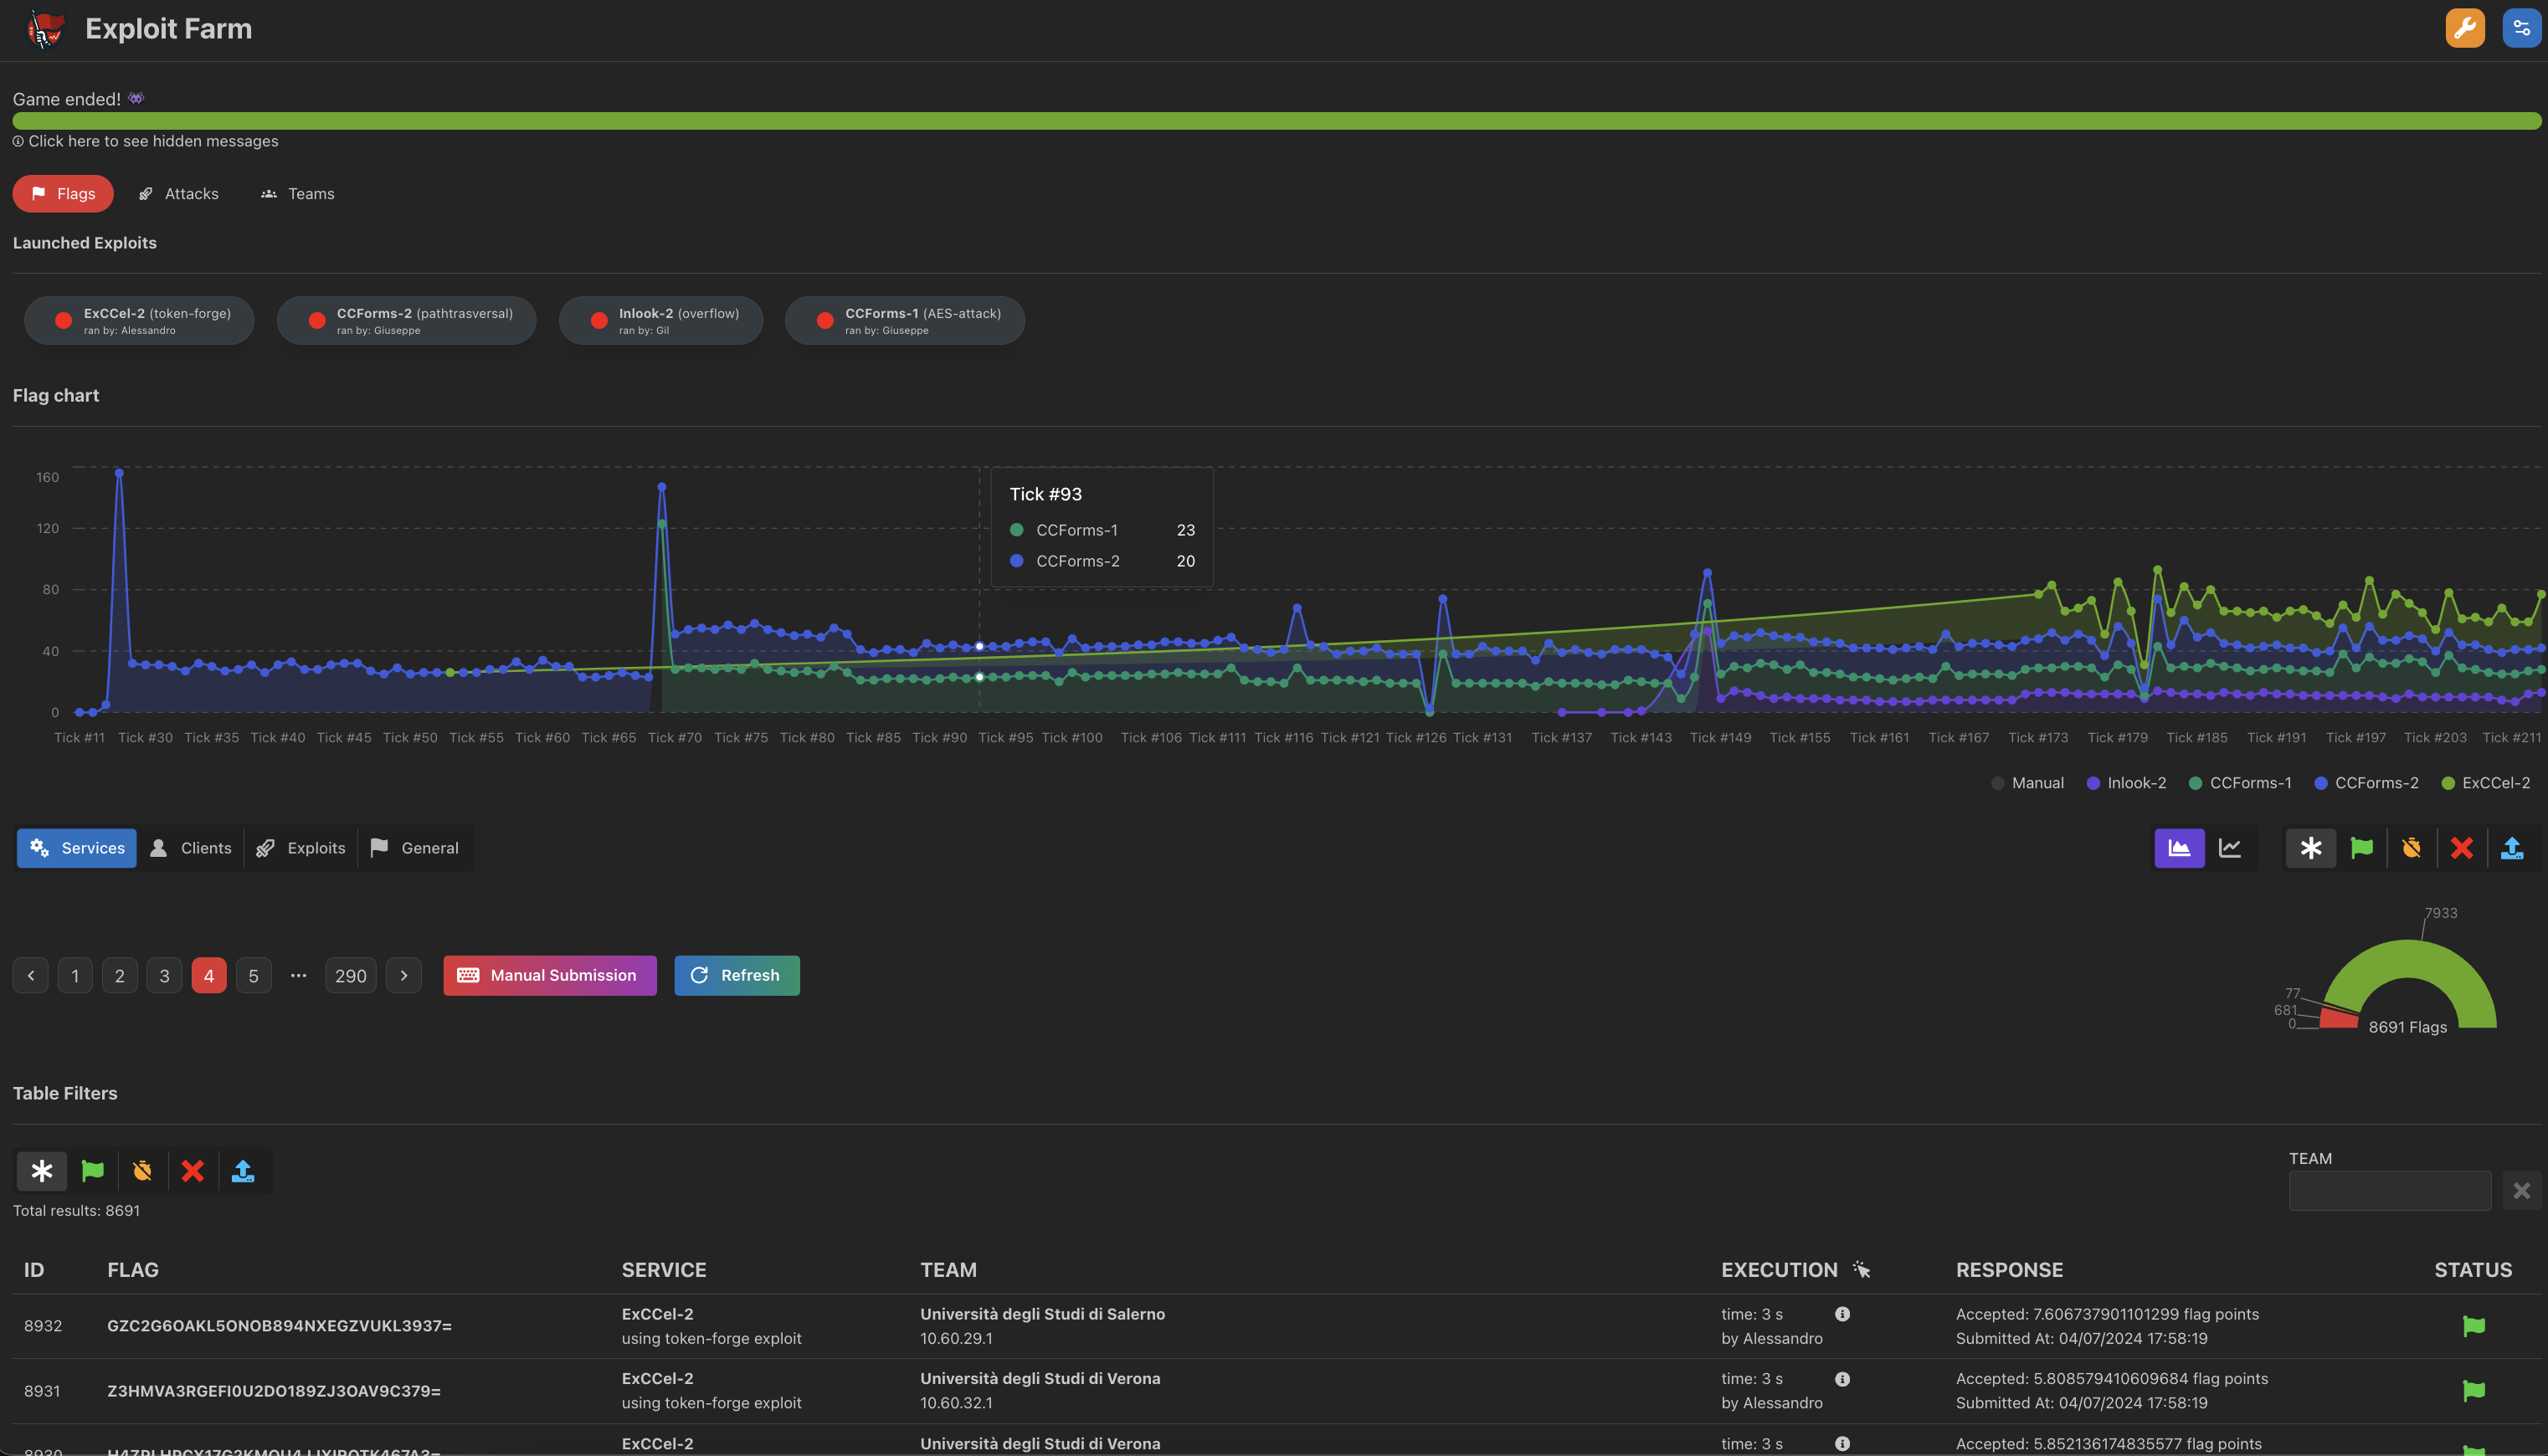
\includegraphics[width=0.98\textwidth]{images/chapter1/exploitfarm_interface.png}
    \caption{Interfaccia di ExploitFarm}\label{fig:exploitfarm_interface}
\end{figure}

\subsection{Proxy e Firewall}

Questi tool permettono di filtrare il traffico in modo da riconoscere e bloccare gli attacchi. Questi tool possono essere molto utili nella difesa, e permettono di bloccare gli attacchi senza di fatto eseguire una modifica sui servizi stessi, spesso diretta conseguenza di malfunzionamenti per errori eseguiti durante questa fase. Questo modo di proteggere i servizi, tuttavia, risulta spesso incompleto e superabile, ma se ben progettato e correttamente utilizzato può essere un'ottima soluzione temporanea, se non una soluzione completa in alcune casistiche specifiche. Spesso però la soluzione più efficace rimane comunque quella di correggere la vulnerabilità. Tool di questo genere sono ad esempio \gls{ctf} Proxy\footcite{\url{https://github.com/ByteLeMani/ctf_proxy}}{ctf_proxy} o il tool di cui tratta questa tesi Firegex\footcite{\url{https://github.com/Pwnzer0tt1/firegex}}{firegex_gh}.

\begin{figure}[H]
    \centering
    
\includegraphics[width=0.20\textwidth]{images/chapter1/FiregexLogo.png}
    \caption{Logo di Firegex}\label{fig:firegex_logo}
\end{figure}

\section{Esempio di un servizio vulnerabile: PCSS}

Consideriamo come esempio un servizio vulnerabile presente nel simulatore di competizioni \gls{ad} CTFBox\footcite{\url{https://github.com/domysh/ctfbox}}{ctfbox_gh}, denominato PCSS (Permanent Cat Storage Service).

Il servizio è composto da un semplice file python e permette di memorizzare e leggere dei testi tramite una connessione \gls{tcp} attraverso un'interfaccia \gls{cli} molto semplice. Il servizio presenta un solo flag store, ma ha al suo interno due vulnerabilità, pertanto per renderlo sicuro è necessario correggerle entrambe.

La registrazione al servizio avviene in modo anonimo: selezionando la funzione di creazione del database, il servizio fornisce un id alfanumerico del database, e un token jwt di accesso con cui è possibile accedere al medesimo in seguito.

Una volta registrati, o eseguito l'accesso tramite il token, è possibile elencare i file presenti nel database, leggerne il contenuto, e crearne nuovi.

A livello tecnico il servizio crea una cartella per ogni database, e all'interno di essa crea i file richiesti.

Il gameserver pubblica come Flag ID l'id del database in cui si trova la flag, e il nome del file in cui è memorizzata.

Come è possibile notare, i flag id non sono sufficienti per accedere alla flag, ma sono un'informazione utile per gli attaccanti per individuare più facilmente la flag all'interno del servizio, e inoltre ci è di aiuto per comprendere dove il servizio memorizza le flag, in questo caso in un file nel database.

La prima vulnerabilità che possiamo individuare è una vulnerabilità di \gls{lfi}:

\begin{listing}[H] 
\begin{minted}[
    frame=single,
    framerule=0.8pt,
    fontsize=\footnotesize,
    breaklines
]{python}
def read_file():
    file = input("Please insert the file name: ").strip()
    print("File content:")
    subprocess.run(["cat", f"./data/{ctx.loggined_db}/{file}"])
    print("")
\end{minted}
\caption{Funzione vulnerabile a Local File Inclusion nel servizio PCSS (da CTFBox\footciteref{ctfbox_gh})}\label{lst:scorecalc}
\end{listing}

Inserendo semplicemente \texttt{`../<database\_id>/<file\_name>'} come nome del file, è possibile accedere a file esterni al database, e quindi anche alla flag.

La seconda vulnerabilità invece è una vulnerabilità di natura crittografica causata dall'uso di una vecchia versione della libreria \texttt{jwt} (versione 0.5.4), che permette di inserire nel token come algoritmo di firma \texttt{none} e quindi di bypassare la verifica della firma, permettendo di generare un token malevolo per accedere al database.

Questo è possibile poichè la prima parte del token \gls{jwt} è in chiaro, e la sua autenticità non è garantita, per cui è usualmente buona pratica specificare lato server quali algoritmi di firma sono supportati, escludendo attacchi di questo tipo. Questa vulnerabilità è la medesima riscontrata in un famoso framework di autenticazione \gls{jwt} in NodeJS e classificata come CVE-2022-23540\footcite{\url{https://nvd.nist.gov/vuln/detail/cve-2022-23540}}{cve_2022_23540}.

È pertanto possibile costruire un token \gls{jwt} valido per accedere al database, e quindi alla flag, senza conoscere il segreto di firma:

\begin{listing}[H]
\begin{minted}[
    frame=single,
    framerule=0.8pt,
    fontsize=\footnotesize,
    breaklines
]{python}
def attack(team_ip: str, flag_id):
    #The bugged jwt is encoded manually but you could also use a jwt lib to make it
    first_part = base64.b64encode(json.dumps({"alg": "none", "typ": "JWT"}).encode()).decode().replace("=", "")
    data_part = base64.b64encode(json.dumps({'db': flag_id['db_name']}).encode()).decode().replace("=", "")
    jwt = f"{first_part}.{data_part}."
    conn = CatStorage(team_ip)
    conn.login(jwt)
    result = conn.read_file(flag_id["filename"])
    conn.close()
    return result
\end{minted}
\caption{Funzione per eseguire un attacco tramite un token JWT malevolo su PCSS (da CTFBox\footciteref{ctfbox_gh})}\label{lst:scorecalc}
\end{listing}

La difesa di questo servizio è piuttosto semplice, ma potrebbe risultare anche facilmente soggetta ad errori che potrebbero comprometterne il funzionamento: ciò potrebbe essere causato dall'aggiornamento della libreria \texttt{jwt} che se soggetta a cambiamenti alle sue \gls{api} nelle versioni successive, potrebbe portare a malfunzionamenti imprevisti del servizio stesso, e quindi necessitare di ulteriori modifiche al servizio.

In alternativa potremmo utilizzare sistemi come firegex\footcite{\url{https://github.com/pwnzer0tt1/firegex}}{firegex_gh} che tramite la sua nuova funzione \gls{nfproxy} può eseguire la decodifica del token \gls{jwt} per verificare che l'algoritmo nel token sia quello previsto dal servizio, interrompendo i tentativi di accesso malevoli. Inoltre filtrando anche i doppi punti nel traffico \gls{tcp} in ingresso, possiamo protteggere il servizio anche dalla vulnerabilità di \gls{lfi}.
\chapter{Firegex}

Firegex è un firewall innovativo e multifunzionale, ideato per essere avviato con 0 configurazioni in modo rapido e semplice, che agisce principalmente a livello applicativo in modo da permettere un'analisi del traffico specifica e dettagliata per ogni servizio. Esistono al suo interno diversi moduli che permettono la creazione di filtri di diversa natura, in modo semplice, flessibile e quanto meno invasivo ed impattante sulle prestazioni della macchina, mantenendo sempre la massima priorità sulla disponibilità e la corretta funzionalità del servizio stesso. Il contesto per cui è stato pensato è quello delle competizioni CTF di tipo Attack/Defense, dove vi sono particolari esigenze (descritte nel capitolo precedente), che Firegex cerca di soddisfare, semplificandone il suo utilizzo, e soprattutto fornendo soluzioni adattabili ai requisiti spesso fortemente dinamici dei servizi in gara.

\begin{figure}[H]
    \centering
    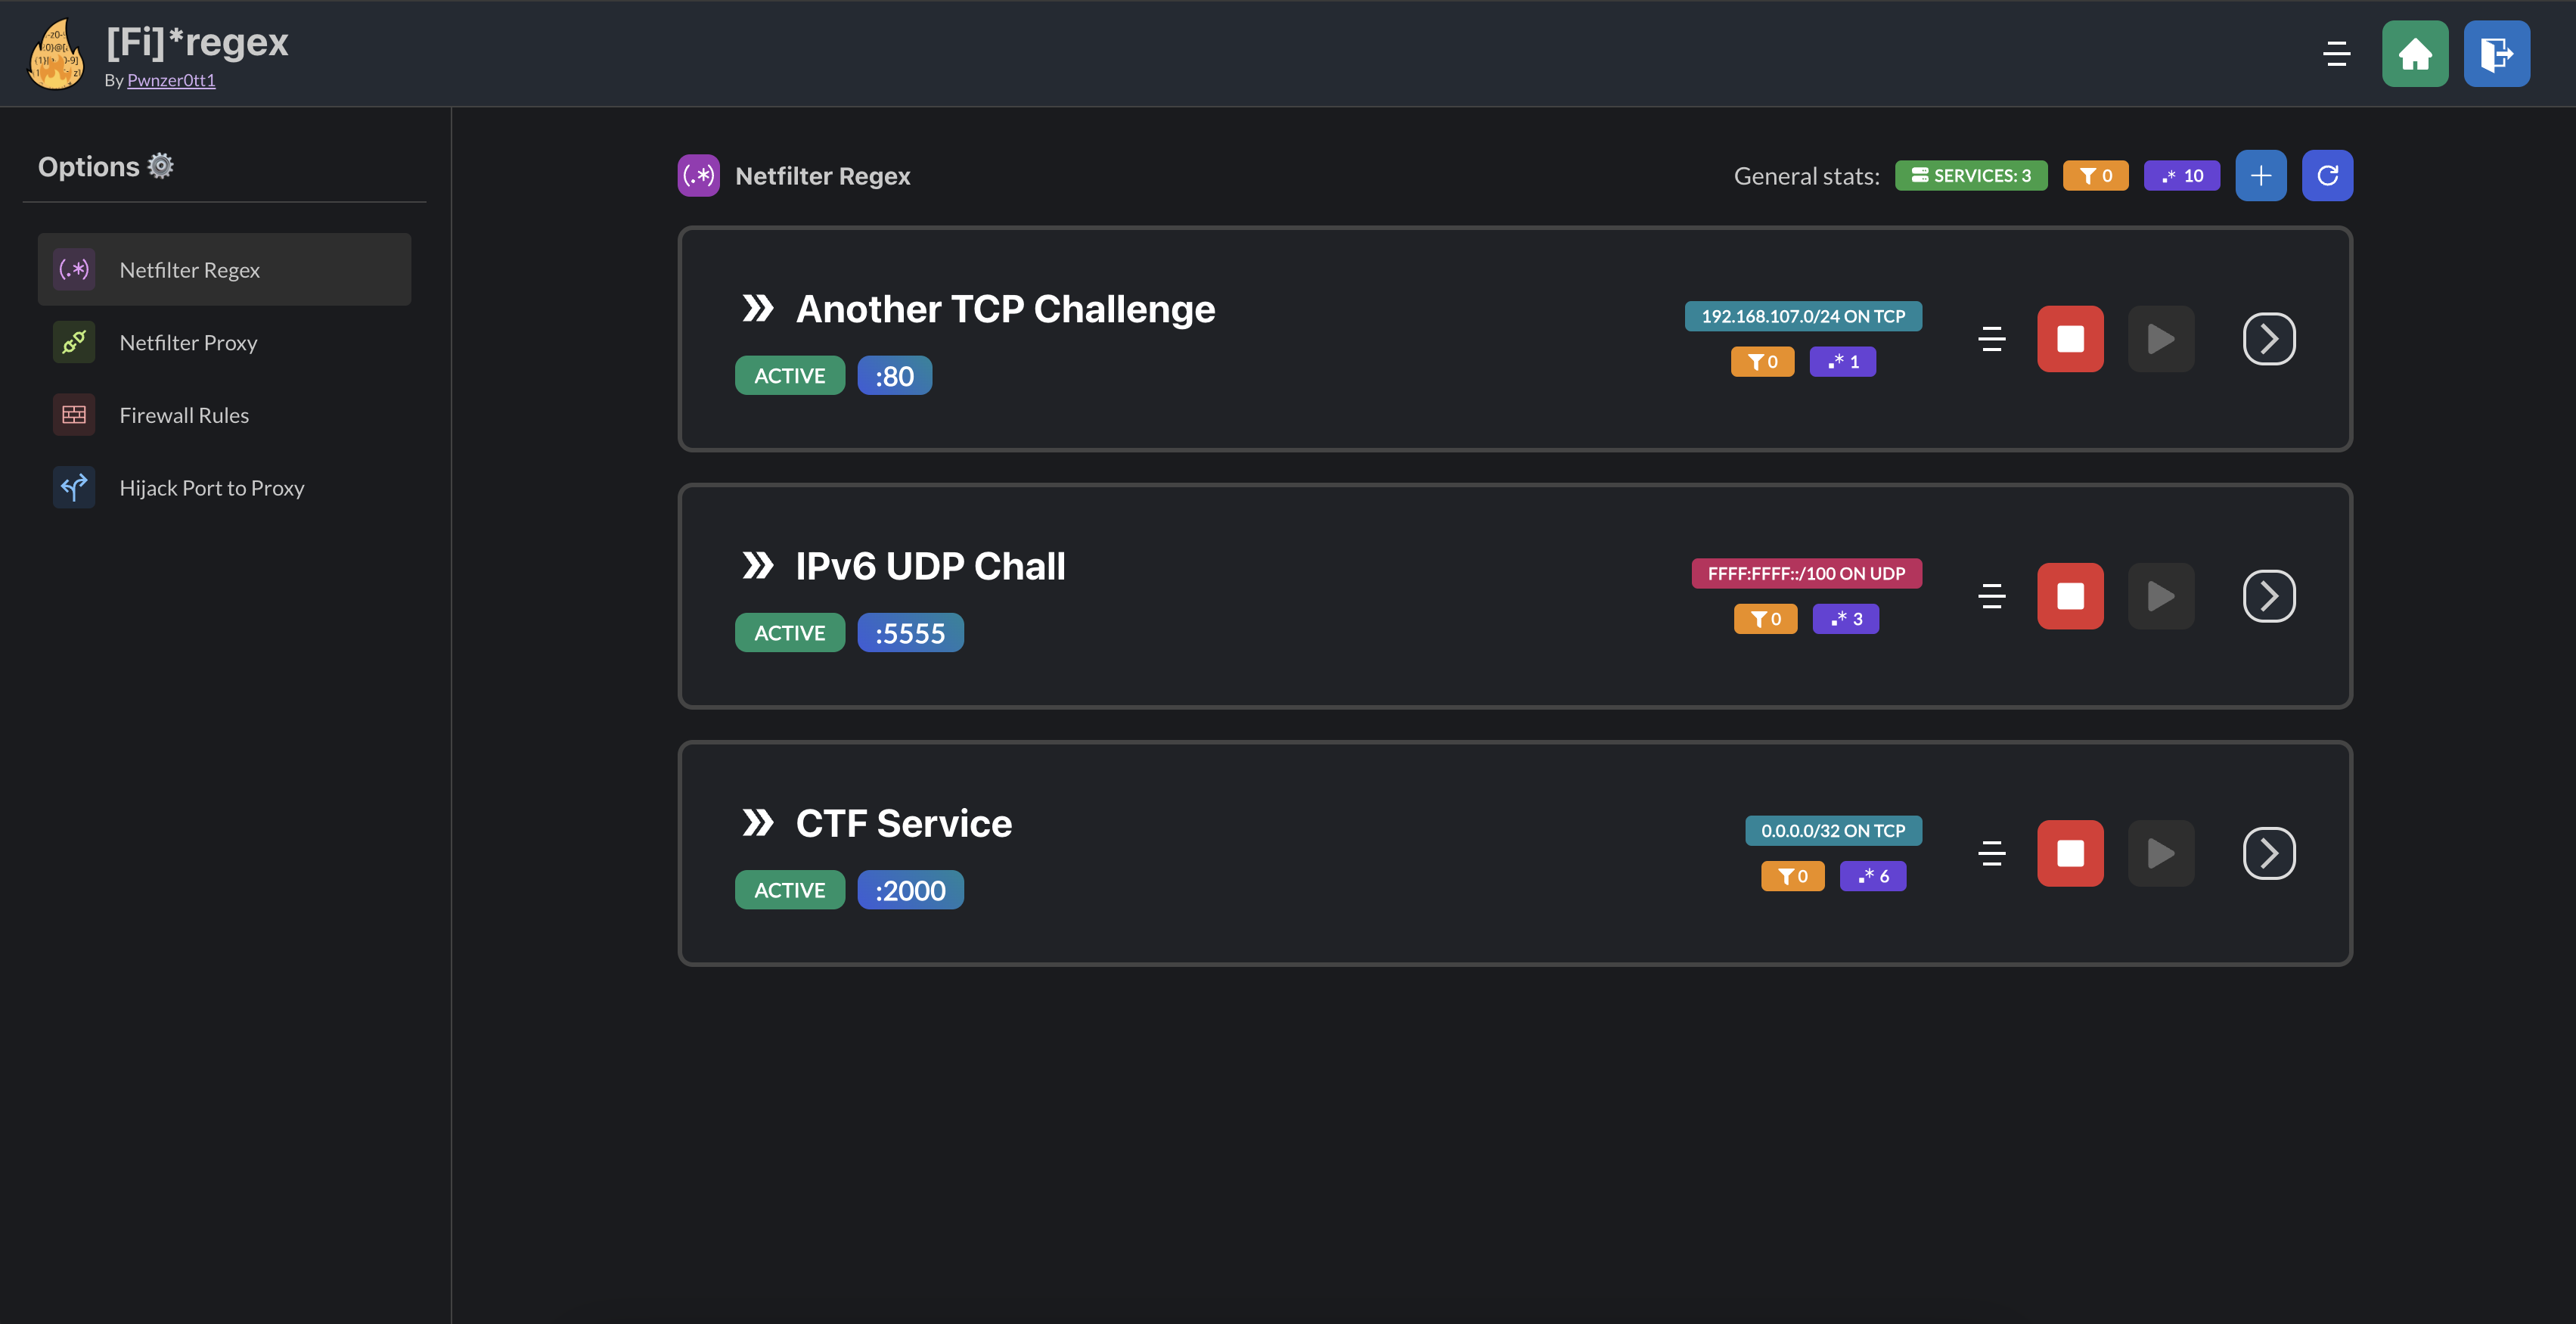
\includegraphics[width=1\textwidth]{images/chapter2/Firegex_Screenshot.png}
    \caption{Interfaccia grafica di Firegex}\label{fig:firegex_frontend}
\end{figure}

\section{Perché nasce Firegex?}

Firegex (come detto in precedenza) nasce dal gruppo che ha affrontato la gara nazionale di Cyberchallenge\footcite{\url{https://cyberchallenge.it/}}{cyberchallenge} del 2022 al Politecnico di Bari\footcite{\url{https://www.poliba.it}}{poliba_website}, come un normale proxy con filtri basati sulle regex, che col tempo si è evoluto aggiungendo nuove funzionalità sempre più efficienti, sicure e funzionali alla competizione stessa.\\
La necessità dello sviluppo è nata proprio dalla mancanza di un sistema di difesa che fosse immediato da utilizzare, che non richiedesse configurazioni complesse per essere avviato, e che permettesse in maniera semplice di costruire dei filtri prontamente attivi, funzionanti e stabili.\\
Durante il suo sviluppo firegex si è sempre più focalizzato su alcuni punti chiave che lo rendono unico rispetto ad altre soluzioni presenti:

\begin{itemize}
    \setlength{\itemsep}{1pt}
    \setlength{\parskip}{1pt}
    \item \textbf{Trasparenza totale:} La creazione di un proxy comporta una serie di cambiamenti sulla configurazione delle porte di rete esposte dai servizi, l'avvio e la gestione del processo del proxy stesso, e utilizzo di meccanismi di fallback per ovviare ad eventuali problematiche. Queste complicanze erano solo parzialmente gestite inizialmente da firegex, ma con le nuove implementazioni è possibile applicare regole sul traffico senza cambiamenti nelle configurazione, grazie a particolari funzionalità utilizzate, disponibili nel kernel linux, nascondendone però tutta la complessità gestita internamente per il loro corretto funzionamento.
    \item \textbf{Integrazione di tecnologie multiple:} Come già detto, Firegex utilizzava come unico meccanismo di filtraggio le regex, che venivano applicate sui pacchetti di rete per individuare eventuali attacchi. Negli anni si è notato come questo approccio spesso potesse essere limitante, per cui sono stati implementati nuovi meccanismi e tecnologie di filtraggio aumentando la precisione con cui è possibile analizzare il traffico. La seguente tesi tratterà dello sviluppo di una nuova funzionalità particolarmente flessibile denominata \texttt{nfproxy}.
    \item \textbf{Affidabilità e disponibilità:} In ambienti dove la continuità del servizio è critica, è fondamentale che il sistema di sicurezza non diventi un collo di bottiglia. Firegex è stato progettato per garantire un’elevata disponibilità, avendo meccanismi di fallback applicati in caso di errori critici, e offrendo soluzioni rapide per il ripristino della configurazione in caso di errori e per il reset immediato dei filtri applicati.
    \item \textbf{Facilità di utilizzo:} Nelle A/D il tempo è una risorsa fondamentale: gli strumenti a disposizione per la gara non devono richiedere eccessivi tempi di configurazione, che tendenzialmente andrebbe automizzata, e facilitare la risoluzione di problemi semplificando eventuali fasi di troubleshooting, che possibilmente andrebbero evitate. L'obiettivo infatti è quello di focalizzare l'attenzione sull'individuazione di vulnerabilità, che rappresenta un necessità chiave nella competizione. Firegex è stato progettato per essere quanto meno dispersivo possibile, avere configurazioni semplici e guidate, un'interfaccia intuitiva, e gestire autonomamente tutte le problematiche legate alla gestione dei filtri e alla loro esecuzione.
\end{itemize}

\section{Confronto con altre soluzioni}

Firegex si distingue rispetto ad altre soluzioni presenti, come \texttt{CTF proxy}\footcite{\url{https://github.com/ByteLeMani/ctf_proxy}}{ctf_proxy}, \texttt{Nginx}\footcite{\url{https://nginx.org/}}{nginx}, \texttt{Suricata}\footcite{\url{https://suricata.io/}}{suricata} o \texttt{Fortinet}\footcite{\url{https://www.fortinet.com/}}{fortinet} per diverse motivazioni:\\

\renewcommand{\arraystretch}{2}
\begin{table}[H]
    \centering
    \setlength{\tabcolsep}{12pt}
    \begin{tabular}{|c|c|c|c|c|}
        \hline
        \begin{tabular}[c]{@{}c@{}} \textbf{Firewall} \end{tabular} & 
        \begin{tabular}[c]{@{}c@{}} \textbf{0 Config Run}  \end{tabular} & 
        \begin{tabular}[c]{@{}c@{}} \textbf{Easy use} \end{tabular} & 
        \begin{tabular}[c]{@{}c@{}} \textbf{Easy Filter Add} \end{tabular} & 
        \begin{tabular}[c]{@{}c@{}} \textbf{Flexible} \end{tabular} \\
        \hline
        \texttt{Firegex} & 
        \begin{tabular}[c]{@{}c@{}} \color{Green}\faIcon[solid]{check-circle} \end{tabular} & 
        \begin{tabular}[c]{@{}c@{}} \color{Green}\faIcon[solid]{check-circle} \end{tabular} & 
        \begin{tabular}[c]{@{}c@{}} \color{Green}\faIcon[solid]{check-circle} \end{tabular} & 
        \begin{tabular}[c]{@{}c@{}} \color{Green}\faIcon[solid]{check-circle} \end{tabular} \\
        \hline
        \texttt{Nginx} & 
        \begin{tabular}[c]{@{}c@{}} \color{Orange}\faIcon[solid]{exclamation-circle} \end{tabular} & 
        \begin{tabular}[c]{@{}c@{}} \color{Orange}\faIcon[solid]{exclamation-circle} \end{tabular} & 
        \begin{tabular}[c]{@{}c@{}} \color{Orange}\faIcon[solid]{exclamation-circle} \end{tabular} & 
        \begin{tabular}[c]{@{}c@{}} \color{Orange}\faIcon[solid]{exclamation-circle} \end{tabular} \\
        \hline
        \texttt{CTF proxy} & 
        \begin{tabular}[c]{@{}c@{}} \color{Red}\faIcon[solid]{times-circle} \end{tabular} & 
        \begin{tabular}[c]{@{}c@{}} \color{Orange}\faIcon[solid]{exclamation-circle} \end{tabular} & 
        \begin{tabular}[c]{@{}c@{}} \color{Orange}\faIcon[solid]{exclamation-circle} \end{tabular} & 
        \begin{tabular}[c]{@{}c@{}} \color{Green}\faIcon[solid]{check-circle} \end{tabular} \\
        \hline
        \texttt{Fortinet} & 
        \begin{tabular}[c]{@{}c@{}} \color{Red}\faIcon[solid]{times-circle} \end{tabular} & 
        \begin{tabular}[c]{@{}c@{}} \color{Red}\faIcon[solid]{times-circle} \end{tabular} & 
        \begin{tabular}[c]{@{}c@{}} \color{Orange}\faIcon[solid]{exclamation-circle} \end{tabular} & 
        \begin{tabular}[c]{@{}c@{}} \color{Orange}\faIcon[solid]{exclamation-circle} \end{tabular} \\ 
        \hline
        \texttt{Suricata} & 
        \begin{tabular}[c]{@{}c@{}} \color{Red}\faIcon[solid]{times-circle} \end{tabular} & 
        \begin{tabular}[c]{@{}c@{}} \color{Orange}\faIcon[solid]{exclamation-circle} \end{tabular} & 
        \begin{tabular}[c]{@{}c@{}} \color{Orange}\faIcon[solid]{exclamation-circle} \end{tabular} & 
        \begin{tabular}[c]{@{}c@{}} \color{Orange}\faIcon[solid]{exclamation-circle} \end{tabular} \\
        \hline
    \end{tabular}
    \caption{Confronto tra le soluzioni per il firewall}\label{tab:firewall_compare}
\end{table}
\renewcommand{\arraystretch}{1}

\begin{itemize}
    \setlength{\itemsep}{1pt}
    \setlength{\parskip}{1pt}
    \item \textbf{Nginx} è una soluzione molto flessibile ed affidabile, ma richiede configurazioni complesse e non permette di applicare filtri in maniera immediata e trasparente, ha necessità di cambiare porte e non supporta nativamente filtri più avanzati come quello trattato in questa tesi. Non ha una interfaccia grafica per la gestione delle regole.
    \item \textbf{CTF proxy} è una soluzione fortemente flessibile, ma richiede la creazione di configurazioni e allo stesso modo necessita di cambiare porte ai servizi originali, inoltre a suo supporto non esiste un'interfaccia semplice da usare.
    \item \textbf{Fortinet} è una soluzione estremamente affidabile, ben riconosciuta nel settore, ma richiede configurazioni complesse ed è per questo molto lento da avviare. Il suo operato inoltre potrebbe causare diversi problemi, essendo molto invasivo nel sistema. Il suo utilizzo è poco pratico per l'utilizzo in competizioni CTF, nonostante rappresenti una delle principali soluzioni fuori da questo contesto.\@
    \item \textbf{Suricata} è una soluzione molto affidabile che offre un grado di flessibilità intermedio, ma pecca della mancanza di un'interfaccia semplice per il suo utilizzo, e richiede configurazioni per essere avviato.
\end{itemize}

\vspace{\fill}
\newpage

\section{Architettura}

Firegex, avendo un interfaccia web, è composto da un frontend scritto in \texttt{react}\footcite{\url{https://react.dev/}}{react} e un backend sviluppato con \texttt{fastapi}\footcite{\url{https://fastapi.tiangolo.com/}}{fastapi}. Il backend utilizza inoltre dei moduli scritti in C++ per le funzionalità più critiche, come per lo scambio dei pacchetti lato kernel e l'elaborazione in tempo reale delle espressioni regolari. Inoltre per funzionare, fa intenso utilizzo delle funzionalità di \texttt{nftables}\footcite{\url{https://netfilter.org/projects/nftables/}}{nftables}, e di \texttt{netfilter\_queue}\footcite{\url{https://netfilter.org/projects/libnetfilter_queue/}}{netfilter_queue} (brevemente \texttt{nfqueue}). L'intera infrastruttura è avviata tramite \texttt{docker}\footcite{\url{https://www.docker.com/}}{docker} che ne permette un avvio con 0 configurazioni e immediato: \texttt{docker} è usualmente lo strumento principale per l'avvio di servizi in competizioni CTF, pertanto nella maggior parte dei casi è già presente e configurato correttamente.

\begin{figure}[H]
    \centering
    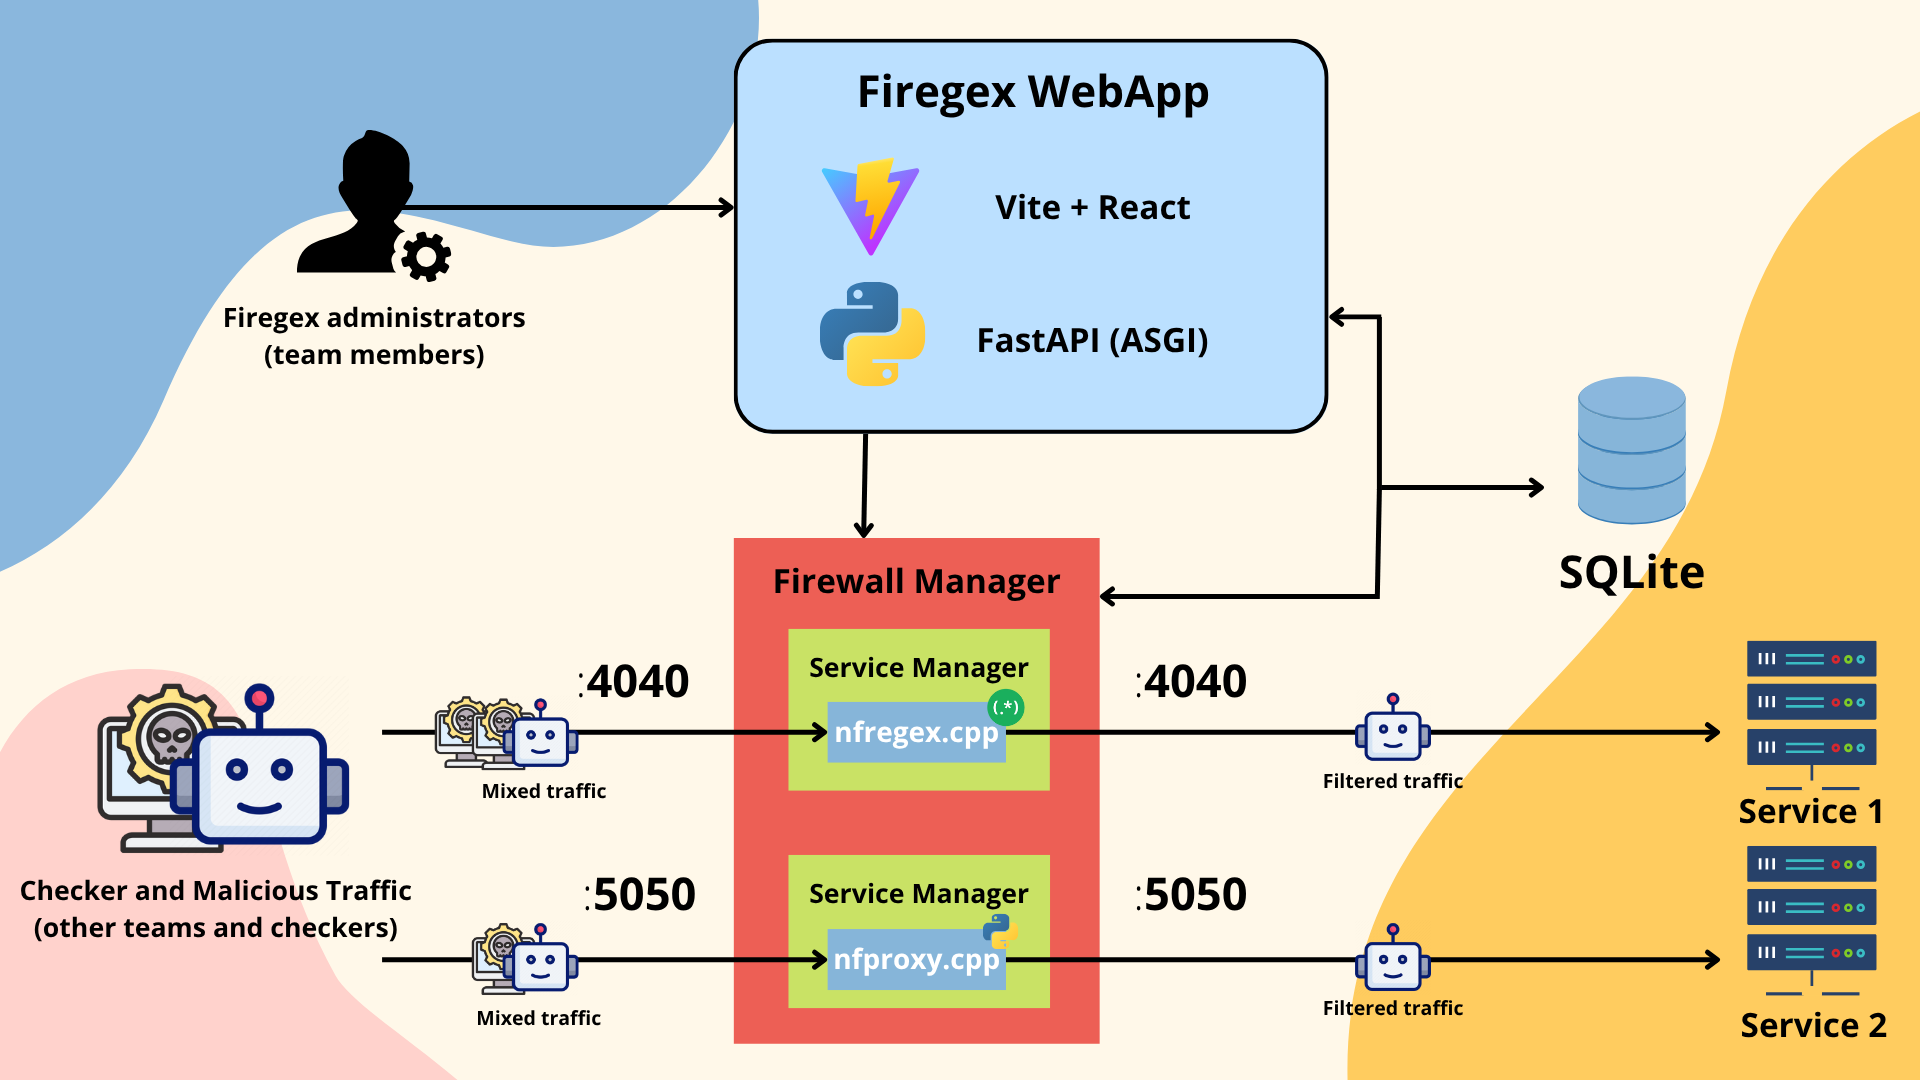
\includegraphics[width=0.98\textwidth]{images/chapter2/FiregexInternals.png}
    \caption{Schema generale dell'architettura di Firegex}\label{fig:firegex_arch}
\end{figure}

\subsection{Frontend e Backend}
\begin{itemize}
    \setlength{\itemsep}{1pt}
    \setlength{\parskip}{1pt}
    \item \textbf{Frontend (React):} L'interfaccia utente risulta fortemente interattiva e intuitiva nelle fasi di creazione dei filtri, nel loro monitoraggio e la gestione degli stessi. L'interfaccia è parte fondamentale di Firegex, poichè consente di soddisfare uno dei punti chiave del progetto: la semplicità di utilizzo.
    \item \textbf{Backend (FastAPI + C++):} Il backend è realizzato utilizzando FastAPI, un framework moderno e ad alte prestazioni per la creazione di API HTTP, integrato con moduli critici scritti in C++. Questa combinazione consente di gestire le richieste in maniera estremamente veloce ed affidabile, garantendo al contempo, l'esecuzione delle operazioni critiche a livello di rete con le performance di un linguaggio a basso livello. Il backend python tuttavia svolge anche un ruolo attivo nell'applicazione delle regole di rete tramite il modulo ufficiale di \texttt{libnftables}\footcite{\url{https://git.netfilter.org/nftables/tree/py}}{nftables_python}.
\end{itemize}

\subsection{Moduli C++}
Le parti critiche di networking gestite da Firegex sono implementate in C++. Questi moduli sono responsabili del filtraggio diretto scambiando pacchetti con il kernel e implementano la logica di filtraggio per i moduli \texttt{nfregex} e \texttt{nfproxy}, facendo utilizzo di librerie ad altre prestazioni come \texttt{libtins}\footcite{\url{https://libtins.github.io/}}{libtins}, \texttt{libmnl}\footcite{\url{https://netfilter.org/projects/libmnl/}}{libmnl}, \texttt{vectorscan}\footcite{\url{https://vectorcamp.gr/project/vectorscan/}}{vectorscan} (specificatamente per \texttt{nfregex}), e le C API di \texttt{python}\footcite{\url{https://docs.python.org/3/c-api/}}{python_c_api} (specificatamente per \texttt{nfproxy}).

Ciò permette di fornire le seguenti caratteristiche:

\begin{itemize}
    \setlength{\itemsep}{1pt}
    \setlength{\parskip}{1pt}
    \item \textbf{Prestazioni elevate:} Grazie all'efficienza del linguaggio C++ e alla possibilità di gestire low level le interazione con il sistema operativo, il filtraggio del traffico avviene con latenze estremamente ridotte.
    \item \textbf{Parallelizzazione:} I filtri che richiedono elaborazione userspace facendo uso di nfqueue, sono gestiti in un sistema di elaborazione multi-thread, garantendo una gestione ottimale del traffico in situazioni di carico elevato e con un numero di connessioni elevate.
    \item \textbf{Integrazione con librerie di rete:} L'utilizzo di librerie specializzate come libtins e libmnl consente di implementare funzionalità avanzate mantenendo affidabilità su come vengono elaborati i pacchetti in rete e prestazioni elevate nell'elaborazione.
\end{itemize}

\subsection{Netfilter nftables}

nftables rappresenta il framework moderno per il filtraggio dei pacchetti e la gestione del traffico nelle distribuzioni Linux. In Firegex, nftables viene utilizzato per:
\begin{itemize}
    \item \textbf{Applicare regole di sicurezza:} Le regole di firewall vengono implementate tramite nftables, garantendo un controllo granulare sul traffico di rete.
    \item \textbf{Reindirizzamento del traffico:} La funzionalità \texttt{porthijack} si basa su regole di nftables per deviare il traffico da una porta a un’altra, consentendo l’implementazione di un proxy interno che si occuperà di filtrare e inoltrare il traffico al servizio originale.
    \item \textbf{Integrazione con nfqueue:} nftables lavora in sinergia con il modulo nfqueue per intercettare i pacchetti e inoltrarli allo spazio utente per ulteriori analisi.
\end{itemize}

Le funzionalità precedentemente citate saranno meglio trattate nei paragrafi successivi.

\subsection{Netfilter Queue Module}
Il modulo Netfilter Queue (nfqueue) gioca un ruolo fondamentale nell'architettura di Firegex, consentendo l'intercettazione dei pacchetti direttamente a livello kernel e il loro inoltro allo spazio utente. Le sue principali caratteristiche includono:
\begin{itemize}
    \setlength{\itemsep}{1pt}
    \setlength{\parskip}{1pt}
    \item \textbf{Intercettazione diretta:} nfqueue permette di catturare il traffico di rete e accodarlo ad una coda, in attesa di essere elaborato da un'applicazione utente: questo permette allo sviluppatore di avere accesso ai pacchetti dal layer di rete, permettendo anche l'analisi e la modifica degli header, normalmente non accessibili tramite un proxy. Inoltre intercettare i pacchetti in questo modo rende l'operazione di filtraggio completamente invisibile per l'applicativo, che non necessiterà di riconfigurazioni.
    \item \textbf{Elaborazione in spazio utente:} Una volta intercettati, i pacchetti vengono inoltrati allo spazio utente dove possono essere analizzati e processati da moduli come \texttt{nfregex} e \texttt{nfproxy}, consentendo l'utilizzo di logiche di filtraggio avanzate ma comunque evitando di portare codice potenzialmente pericoloso lato kernel che potrebbe compromettere la stabilità del sistema.
\end{itemize}

\section{Funzionalità}

All'interno di Firegex sono presenti attualmente 4 moduli principali, ognuno con delle funzionalità specifiche che permettono di applicare filtri con tecnologie e funzionalità differenti. I moduli sono \texttt{nfregex}, \texttt{firewall}, \texttt{porthijack} e \texttt{nfproxy}. All'interno di questi moduli firegex possiede una documentazione interna alla piattaforma stessa che permette di comprendere come utilizzare le funzionalità offerte, e come configurare i filtri in maniera corretta.\\
Firegex è avviabile tramite un unico comando, supponendo che \texttt{docker}\footcite{\url{https://www.docker.com/}}{docker} sia stato già installato nel sistema:

\begin{listing}[H]
    \begin{minted}[
        frame=single,
        framerule=0.8pt,
        fontsize=\footnotesize,
        breaklines
      ]{bash}
sh <(curl -sLf https://pwnzer0tt1.it/firegex.sh)
\end{minted}
\end{listing}

\subsection{nfregex}
Il modulo \texttt{nfregex} (pensato originariamente come unico e principale) possiede funzionalità per la creazione di filtri basati su espressioni regolari. Utilizzando \texttt{nfqueue} in combinazione con \texttt{nftables}, questo modulo intercetta le richieste di rete direttamente a livello kernel. La funzionalità permette l'utilizzo di regex \texttt{PCRE2}\footcite{\url{https://www.pcre.org/}}{pcre_website} compliant tramite l'utilizzo di \texttt{vectorscan}\footcite{\url{https://vectorcamp.gr/project/vectorscan/}}{vectorscan} (fork di \texttt{hyperscan}\footcite{\url{http://hyperscan.io/}}{hyperscan} compatibile con arm64) per garantire prestazioni elevate e una corretta elaborazione delle regole. La funzionalità supporta IPv4 e IPv6, e protocolli di livello superiore come TCP e UDP.\@ Per i pacchetti TCP, la regex viene applicata all'intero flusso ricostruito e ordinato, tramite le \texttt{stream regex} disponibili in vectorscan.

\subsection{firewall}
La funzionalità \texttt{firewall} di Firegex offre un controllo completo sul traffico di rete, tramite regole simili a quelle offerte da strumenti che agiscono a livello di rete e di trasporto come \texttt{ufw} o \texttt{iptables}. Dispone quindi di funzionalità basilari e risulta utile per applicare questa tipologia di regole evitando ulteriori tool di filtering che potrebbero entrare in conflitto con firegex.

\subsection{porthijack}
Il modulo \texttt{porthijack} introduce la capacità di reindirizzare il traffico destinato ad una determinata porta verso un’altra. Questa funzionalità è particolarmente utile in scenari dove si ha il bisogno di costruire un proxy personalizzato, ma si vuole evitare la riconfigurazione del servizio di base. Port hijacking infatti consente di impostare un redirect del traffico dall'interfaccia su cui il servizio viene esposto nella rete di gara, dirottandolo per un proxy in localhost, che poi tramite la stessa interfaccia di loopback inoltrerà il traffico al servizio originale.

\subsection{nfproxy}
\texttt{nfproxy}, il modulo trattato in questa tesi, sfrutta le funzionalità di \texttt{nfqueue} per l'intercettazione del traffico, simulando lato utilizzatore il comportamento di un tradizionale proxy python. Le caratteristiche principali del modulo sono:
\begin{itemize}
    \setlength{\itemsep}{1pt}
    \setlength{\parskip}{1pt}
    \item \textbf{Sviluppo in Python:} Permette agli sviluppatori di scrivere e integrare filtri personalizzati in linguaggio Python, offrendo un altissimo livello di flessibilità per l'analisi del traffico.
    \item \textbf{Parsing avanzato dei protocolli:} Tramite funzionalità predefinite è possibile eseguire la decodifica di protocolli come HTTP, in modo immediato e già disponibile all'utilizzo, senza che queste funzionalità debbano essere implementate manualmente.
    \item \textbf{Test e validazione:} I filtri possono essere provati in anticipo tramite il comando \texttt{fgex}, rendendo possibile la prova del filtro prima si applicarlo al traffico.
    \item \textbf{Interfaccia grafica:} L'interfaccia di dettaglio del servizio permette di visualizzare in tempo reale i log e le eventuali eccezioni che si verificano durante l'esecuzione del filtro.
\end{itemize}

Il seguente modulo è stato introdotto in vista di scenari complessi dove gli elementi da individuare per il corretto filtraggio non sono facilmente individuabili tramite regex: ad esempio se il payload fraudolento fosse in dei token JWT, sarebbe necessario eseguire il decoding per rilevare l'attacco.

\begin{figure}[H]
    \centering
    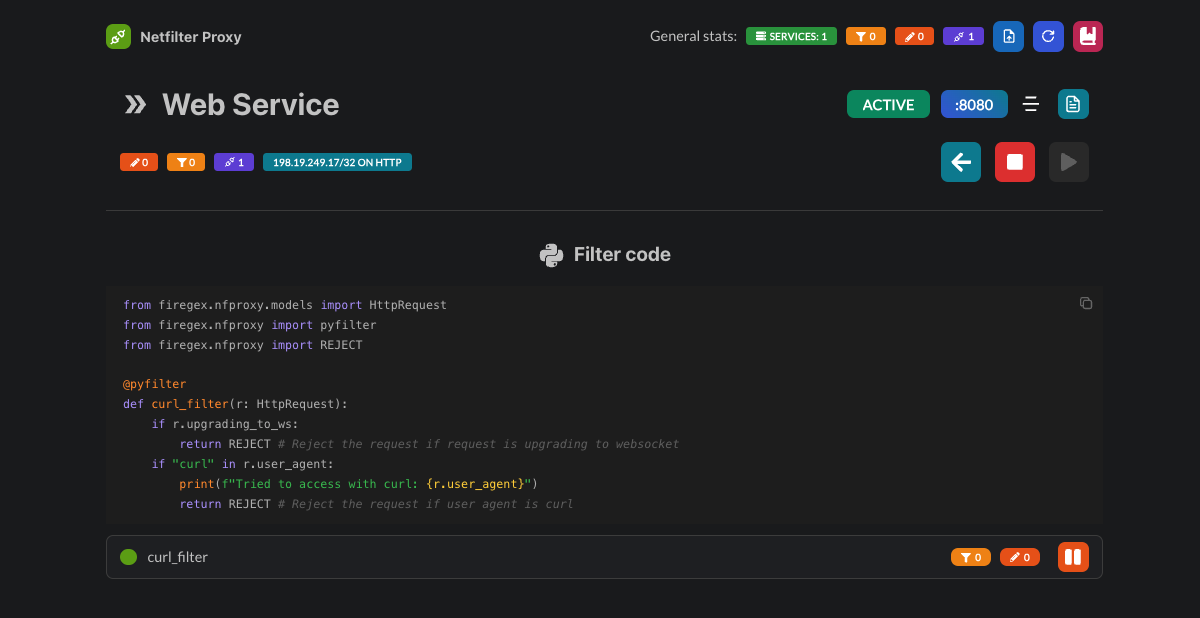
\includegraphics[width=0.83\textwidth]{images/chapter2/NFProxyInterface.png}
    \caption{Interfaccia di dettaglio del servizio nel modulo nfproxy}\label{fig:nfproxy_interface}
\end{figure}

Nei prossimi capitoli verrà trattato in dettaglio lo sviluppo di \texttt{nfproxy}, le sue funzionalità, le problematiche affrontate e le soluzioni adottate.

\chapter{Progettazione e sviluppo del modulo nfproxy}\label{chap:nfproxy}

Il \gls{regex} filtering è un modello di filtraggio che garantisce ottime prestazioni (grazie all'elaborazione tramite linguaggi e librerie ottimizzati), ma presenta forti limitazioni nella flessibilità di analisi del traffico.

Questa rigidità è particolarmente rilevante nei \gls{ctf}, dove la maggior parte dei servizi utilizza protocolli come \gls{http}, che spesso includono contenuti compressi o codificati (es. Base64, \gls{gzip}), difficilmente analizzabili tramite \gls{regex}.

A discapito delle prestazioni, \gls{nfproxy} introduce il vantaggio di scrivere filtri in Python\footcite{\url{https://python.org/}}{python}, linguaggio semplice e rapido per lo scripting, superando i limiti precedentemente descritti e offrendo:

\begin{itemize}
    \setlength{\itemsep}{4pt}
    \setlength{\parskip}{4pt}
    \item Massima libertà nell'implementazione delle logiche di filtraggio
    \item Prestazioni comunque elevate grazie a scelte architetturali mirate
    \item Supporto nativo a compressioni/encoding comuni, tramite il parsing del protocollo applicativo
\end{itemize}

\gls{nfproxy} non è un proxy tradizionale ma un modulo basato su
\gls{nfqueue}\footcite{\url{https://netfilter.org/projects/libnetfilter_queue/}}{netfilter_queue},
che permette un controllo sul traffico paragonabile ad un proxy classico, ma con accesso diretto ai pacchetti a livello di rete (layer 3/4) e con un'intercettazione del traffico invisibile all'applicativo.

Va riportata l'esistenza di limitazioni nella modifica dei pacchetti, che tuttavia non rappresenta uno scenario d'uso necessario per la difesa del servizio.

Il sistema combina C++ per un gestione efficiente dei pacchetti e Python per eseguire il parsing dei protocolli applicativi.

Questo approccio ibrido permette di sfruttare al meglio le caratteristiche di entrambi i linguaggi, garantendo prestazioni elevate e flessibilità nello sviluppo dei filtri.

I protocolli attualmente supportati includono:
\begin{itemize}
    \setlength{\itemsep}{4pt}
    \setlength{\parskip}{4pt}
    \item \gls{http}/1.1\footcite{RFC2616, Hypertext Transfer Protocol -- HTTP/1.1}{rfc2616} (con gestione compressione/encoding del body)
    \item Websocket\footcite{RFC6455, The WebSocket Protocol}{rfc6455} (con decodifica dei frame e supporto alle estensioni)
    \item \gls{tcp} standard\footcite{RFC9293, Transmission Control Protocol (TCP)}{rfc9293} (con ricostruzione dello stream)
\end{itemize}

\section{Requisiti}

Di seguito gli obiettivi fondamentali del modulo:

\begin{itemize}
    \setlength{\itemsep}{4pt}
    \setlength{\parskip}{4pt}
    
    \item \textbf{Integrazione con Python}: Fornire un'interfaccia in Python per implementare le regole di filtraggio, con funzioni ottimizzate e sintassi intuitiva.
    
    \item \textbf{Analisi avanzata di \gls{http}/1.1 e WebSocket}: Interpretazione nativa dei pacchetti applicativi, con estrazione automatica dei dati decodificati/decompressi. Supporto integrato per:
    \gls{gzip}\footcite{RFC1952, GZIP file format specification version 4.3}{rfc1952},
    deflate\footcite{RFC1951, DEFLATE Compressed Data Format Specification version 1.3}{rfc1951},
    brotli\footcite{RFC7932, Brotli Compressed Data Format}{rfc7932},
    \gls{zstd}\footcite{RFC8478, Zstandard Compression and the application/zstd Media Type}{rfc8478}, 
    e l'estensione WebSocket permessage-deflate\footcite{RFC7692, Compression Extensions for WebSocket}{rfc7692}.
    
    \item \textbf{Ricostruzione dello stream TCP}: Accesso al payload ordinato a livello di trasporto, indipendentemente dalla frammentazione.
    
    \item \textbf{Manipolazione degli header}: Lettura e modifica diretta dei campi negli header di rete (\gls{ip}) e trasporto (\gls{tcp}).
    
    \item \textbf{Compatibilità dual-stack}: Elaborazione sia di pacchetti \gls{ipv4}\footcite{RFC791, Internet Protocol}{rfc791} che \gls{ipv6}\footcite{RFC2460, Internet Protocol, Version 6 (\gls{ipv6}) Specification}{rfc2460}.
    
    \item \textbf{Allocazione e deallocazione di memoria ottimizzata}: Gestione automatica dei buffer per evitare memory leak e sovraccarichi, non delegandone la gestione al programmatore, ma fornendo opzioni di configurazione opzionali per configurare il modo in cui vengono gestiti.
    
    \item \textbf{Diagnostica avanzata}: Notifica strutturata degli errori (codici, descrizioni, contesto) con log dettagliati per l'analisi forniti in tempo reale.
    
    \item \textbf{Modifica dinamica delle regole}: Attivazione/disattivazione istantanea dei filtri (anche solo di alcuni specifici) senza interrompere il servizio.
    
    \item \textbf{Elaborazione parallela}: Distribuzione del carico su multipli core \gls{cpu} per garantire scalabilità lineare.
    
    \item \textbf{Testing dei filtri tramite simulazione}: Verifica delle regole in un ambiente simulato per debugging da poter utilizzare in fase di sviluppo e verifica dei filtri.
\end{itemize}

\vspace{\fill}
\newpage

\section{Architettura}

Il modulo \gls{nfproxy} viene avviato dal backend di Firegex attraverso un processo articolato in tre fasi principali.

In primo luogo, il backend configura le regole di \gls{nftables}\footcite{\url{https://netfilter.org/projects/nftables/}}{nftables} mediante chiamate alle sue \gls{api} \gls{json}.\@ Successivamente, viene inizializzato il componente C++ responsabile della logica centrale, che include la gestione del multi-threading, l'elaborazione a basso livello dei pacchetti e la ricostruzione degli stream \gls{tcp}.\@ Nella fase finale, vengono caricati e applicati dinamicamente i filtri Python definiti dall'utente. L'architettura completa del modulo è rappresentata nella Figura~\ref{fig:firegex_nfproxy_arch}, dove si evince l'interazione tra i tre livelli (configurazione, core C++ e strato Python).

\begin{figure}[H]
    \centering
    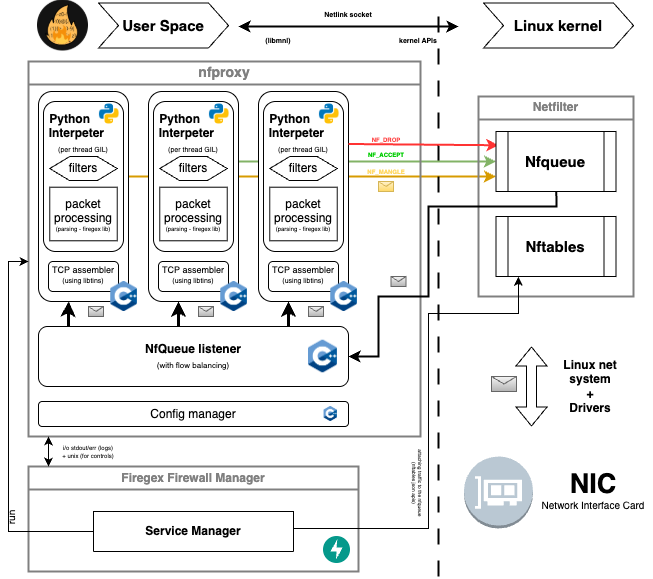
\includegraphics[width=0.9\textwidth]{images/chapter3/nfproxy.drawio.png}
    \caption{Architettura del modulo \gls{nfqueue}}\label{fig:firegex_nfproxy_arch}
\end{figure}

\section{Elaborazione parallelizzata dei pacchetti}

Uno dei principali ostacoli progettuali ha riguardato la parallelizzazione dei processi di elaborazione, legata a tre fattori critici:  
il funzionamento intrinseco di \gls{nfqueue}, alcune peculiarità del linguaggio Python e l'integrazione ibrida C++/Python.

Tre obiettivi hanno guidato l'implementazione della parallelizzazione:  

\begin{itemize}
    \setlength{\itemsep}{2pt}
    \setlength{\parskip}{2pt}
    \item \textbf{Isolamento dei dati tra processi}: Prevenire conflitti interprocesso per evitare corruzione dati, crash imprevisti e comportamenti anomali
    \item \textbf{Minimizzazione dei lock}: Limitare l'uso di meccanismi di blocco (pur necessari per risorse condivise) per prevenire deadlock e un degrado delle prestazioni
    \item \textbf{Ottimizzazione della memoria}: Eliminare copie ridondanti dei pacchetti e processi superflui, massimizzando throughput e riducendo la latenza
\end{itemize}

La soluzione adottata segue il pattern produttore-consumatore. Un processo produttore unico, responsabile del binding alla \gls{nfqueue},
riceve i pacchetti dal kernel e li distribuisce a multiple code \gls{fifo}.\@ I consumatori, associati ciascuno ad una coda dedicata, gestiscono in parallelo:
\begin{itemize}
    \setlength{\itemsep}{2pt}
    \setlength{\parskip}{2pt}
    \item Ordinamento dei pacchetti \gls{tcp}  
    \item Applicazione dei filtri Python  
    \item Invio dei verdicts\footcite{\url{https://netfilter.org/projects/libnetfilter_queue/doxygen/html/group__nfq__verd.html}}{vedicts_nfqueue} al kernel
\end{itemize}

L'unica sezione critica risiede nell'accesso concorrente alle code, protetto da un sistema di lock basato su
std::mutex\footcite{\url{https://en.cppreference.com/w/cpp/thread/mutex}}{std_mutex} e std::condition\_variable\footcite{\url{https://en.cppreference.com/w/cpp/thread/condition_variable}}{condition_variable_std}. Questa scelta, preferita alle unix pipe\footcite{\url{https://man7.org/linux/man-pages/man2/pipe.2.html}}{unix_pipe} per motivi prestazionali, implementa inoltre un meccanismo di backpressure che blocca il produttore in caso di code sature, prevenendo un consumo eccessivo di memoria.

L'implementazione si basa su quella pubblicata da Arif Jaffer\footcite{\url{https://www.bit-byter.com/blog/files/blocking-q-cpp.html}}{blocking_queue_cpp} per le code bloccanti.

\subsection{A Per-Interpreter Global Interpreter Lock}

Una delle problematiche citate precedentemente sulla parallelizzazione riguardava una caratteristica del linguaggio Python: il \gls{gil}\footcite{Understanding the python gil}{beazley2010understanding} (Global Interpreter Lock). Questo meccanismo limita l'utilizzo dei thread consentendo l'esecuzione di un solo thread alla volta, necessario per prevenire conflitti nella gestione interna degli oggetti Python (come il reference counting) che non è implementata in modo thread-safe.

Si osserva inoltre come, in questo specifico contesto, Python gestisca operazioni \emph{\gls{cpu}-bound}, accentuando ulteriormente gli svantaggi del \gls{gil}.\@

\begin{figure}[H]
    \centering
    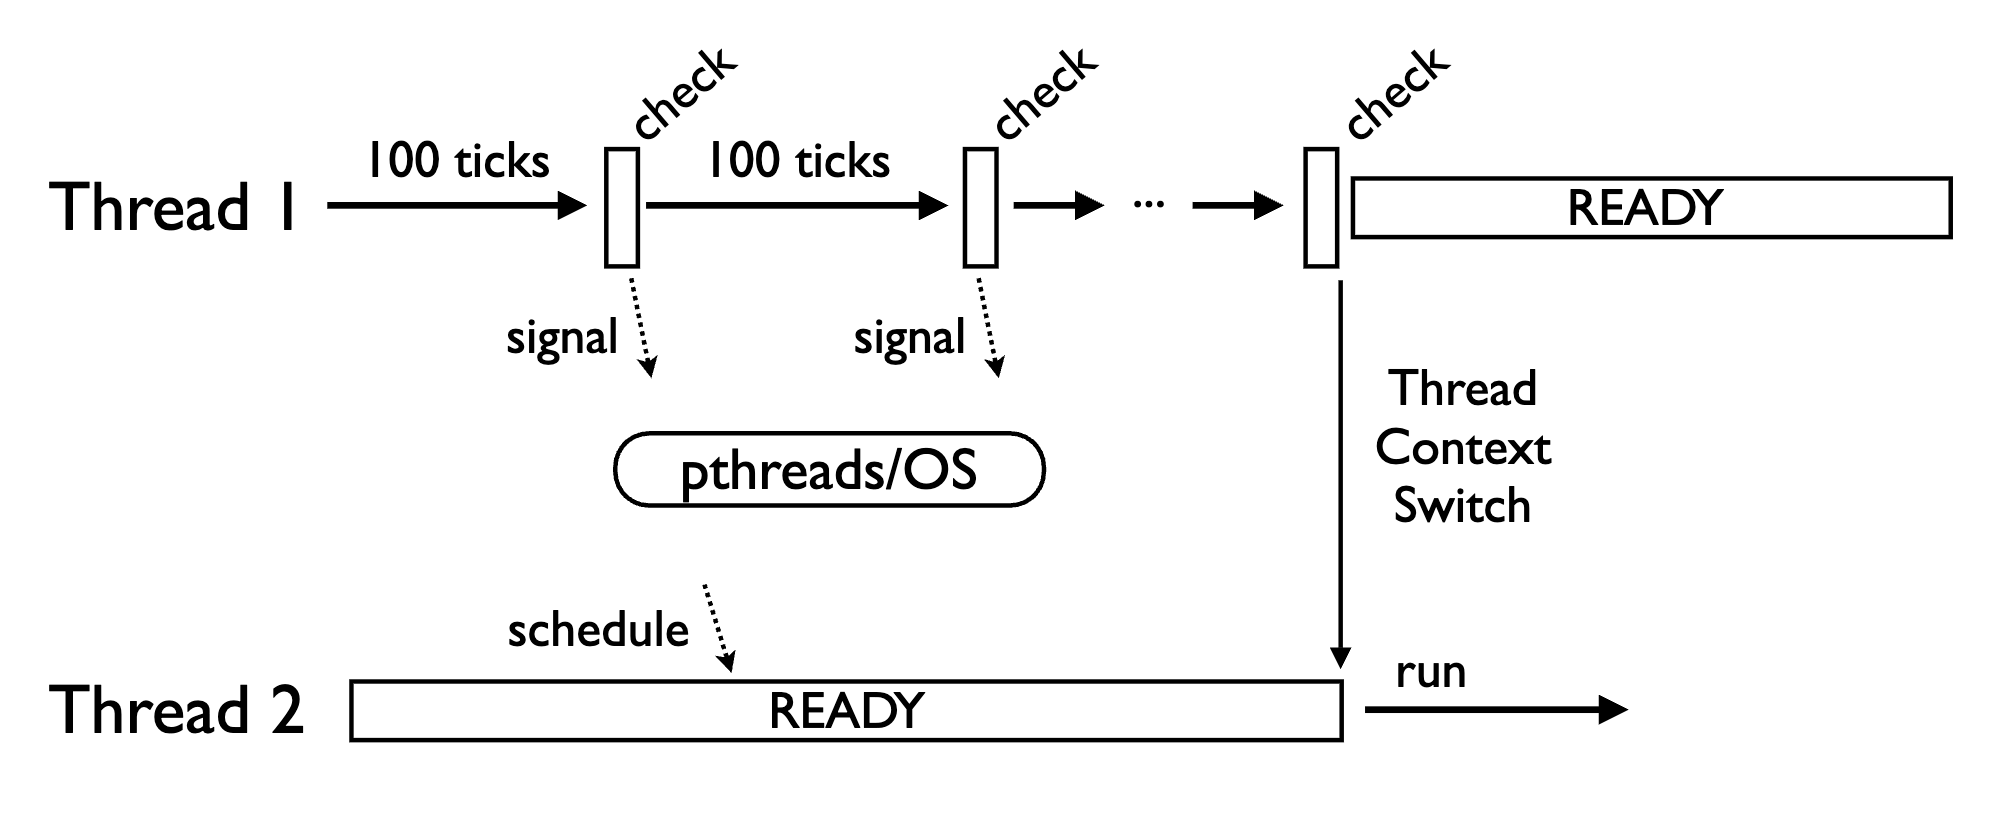
\includegraphics[width=0.98\textwidth]{images/chapter3/GIL.png}
    \caption{Python Global Interpreter Lock}\label{fig:py_gil_schema}
\end{figure}

Una soluzione alternativa potrebbe essere l'uso di processi multipli (con \gls{gil} separati per processo), approccio che tuttavia introdurrebbe overhead dovuti
alla comunicazione inter-processo e alla duplicazione della memoria.

La soluzione adottata sfrutta il \gls{pep} 684\footcite{\url{https://peps.python.org/pep-0684/}}{pep648} introdotto in Python 3.12, che permette l'esecuzione
di interpreti Python indipendenti nello stesso processo, ciascuno con il proprio \gls{gil}.\@ L'attivazione di questa funzionalità avviene esclusivamente tramite C-\gls{api}, consentendo:
\begin{itemize}
    \setlength{\itemsep}{2pt}
    \setlength{\parskip}{2pt}
    \item Avvio diretto di interpreti via libpython
    \item Integrazione trasparente tra codice C++ e Python
    \item Parallelismo reale senza overhead di processi multipli
\end{itemize}
L'impossibilità di condividere oggetti tra interpreti, uno dei limiti di questo approccio, non costituisce un problema nel nostro caso poichè, grazie al meccanismo di
smistamento dei pacchetti descritto nel prossimo paragrafo, ciò non sarà necessario.

Per ogni nuova connessione \gls{tcp} vengono eseguite le seguenti operazioni:\@
\begin{itemize}
    \setlength{\itemsep}{2pt}
    \setlength{\parskip}{2pt}
    \item Viene inizializzato un nuovo contesto globale Python indipendente
    \item Il bytecode del filtro, precedentemente compilato, viene deserializzato tramite le funzionalità di marshaling\footcite{\url{https://docs.python.org/3/library/marshal.html}}{marshal_python}
    \item Il codice di inizializzazione del filtro viene eseguito sul contesto globale
\end{itemize}

\begin{listing}[H]
\begin{minted}[
    frame=single,
    framerule=0.8pt,
    fontsize=\footnotesize,
    breaklines
]{cpp}
// Configurazione interprete con GIL indipendente
PyInterpreterConfig py_thread_config = {
    .use_main_obmalloc = 0,
    .allow_fork = 0,
    .allow_exec = 0,
    .allow_threads = 0,
    .allow_daemon_threads = 0,
    .check_multi_interp_extensions = 1,
    .gil = PyInterpreterConfig_OWN_GIL,
};

void before_loop() {
    PyStatus pystatus;
    tstate = PyThreadState_New(PyInterpreterState_Main());
    PyEval_AcquireThread(tstate); // Acquisizione GIL
    pystatus = Py_NewInterpreterFromConfig(&tstate, &py_thread_config);
    handle_packet_code = unmarshal_code(...); // Deserializzazione bytecode
}
\end{minted}
\caption{Inizializzazione di un processo consumatore con GIL indipendente in nfproxy}\label{lst:no_gil_python_nfproxy}
\end{listing}
L'utilizzo delle funzionalità offerte dal \gls{pep} 684\footcite{\url{https://peps.python.org/pep-0684/}}{pep648}, soffre tuttavia anche di forti limitazioni sull'utilizzo di moduli senza multi-phase initialization\footcite{\url{https://peps.python.org/pep-0489/}}{pep489} (includendo tutti quelli scritti in Cython\footcite{\url{https://cython.org/}}{cython}) e moduli con componenti non thread-safe. Nel corso dello sviluppo, queste limitazioni sono state oggetto di diverse problematiche, affrontate e approfondite in seguito.

Un'altra possibilità considerata è stata l'utilizzo dell'interprete in free-threaded mode di Python 3.13\footcite{\url{https://docs.python.org/3/whatsnew/3.13.html\#whatsnew313-free-threaded-cpython}}{py13_free_threaded}, attualmente sconsigliato per:
\begin{itemize}
    \setlength{\itemsep}{2pt}
    \setlength{\parskip}{2pt}
    \item Lo stato sperimentale della feature
    \item Calo prestazionale dovuto alla disattivazione temporanea di alcuni sistemi di ottimizzazione del linguaggio
    \item Incompatibilità con molti moduli CPython
\end{itemize}

\subsection{Bilanciamento del carico}

Per il bilanciamento del carico tra i processi consumatori, finalizzato all'isolamento e alla distribuzione equa dei pacchetti, è stato implementato un meccanismo di hashing basato su indirizzi \gls{ip} e porte di origine/destinazione. Questo approccio garantisce una distribuzione uniforme dei pacchetti tra i consumatori, evitando sovraccarichi e assicurando un'elaborazione parallela efficiente, oltre che a instradare i pacchetti di una stessa connessione sempre verso lo stesso thread.

\begin{listing}[H]
\begin{minted}[
    frame=single,
    framerule=0.8pt,
    fontsize=\footnotesize,
    breaklines
]{cpp}
uint32_t hash_stream_id(const stream_id &sid) {
    uint32_t addr_hash = 0;
    addr_hash ^= min_addr[0] ^ min_addr[1] ^ min_addr[2] ^ min_addr[3];
    addr_hash ^= max_addr[0] ^ max_addr[1] ^ max_addr[2] ^ max_addr[3];
    uint32_t ports = (static_cast<uint32_t>(sid.min_address_port) << 16) | sid.max_address_port;
    uint32_t hash = addr_hash ^ ports;
    hash *= 0x9e3779b9; // Aggiunta di entropia (moltiplicazione con numero primo)
    return hash;
}

// Funzione di bilanciamento semplificata
void __real_handler(PktRequest<Worker>* pkt) {
    const size_t idx = hash_stream_id(pkt->sid) % pkt->ctx->size();
    converted_pkt->ctx->queue.put(converted_pkt);
}
\end{minted}
\caption{Funzione di hashing per stream\_id (valida per IPv4/IPv6) in \gls{nfproxy}}\label{lst:nfproxy_hash}
\end{listing}

La tecnica riprende i meccanismi di bilanciamento usati kernel space da \gls{nfqueue}, che tuttavia non considera le porte di origine/destinazione,
limitandosi ad un hashing basato solo sugli indirizzi \gls{ip}.\@ Ciò è dovuto alla necessità di adattare l'algoritmo anche a protocolli diversi da \gls{tcp} e \gls{udp}, come \gls{icmp} che non prevede porte.

\begin{listing}[H]
\begin{minted}[
    frame=single,
    framerule=0.8pt,
    fontsize=\footnotesize,
    breaklines
]{cpp}
static inline u32
nfqueue_hash(const struct sk_buff *skb, u16 queue, u16 queues_total, u8 family,
	     u32 initval)
{
	switch (family) {
	case NFPROTO_IPV4:
		queue += reciprocal_scale(hash_v4(ip_hdr(skb), initval),
					  queues_total);
		break;
	case NFPROTO_IPV6:
		queue += reciprocal_scale(hash_v6(ipv6_hdr(skb), initval),
					  queues_total);
		break;
	case NFPROTO_BRIDGE:
		queue += reciprocal_scale(hash_bridge(skb, initval),
					  queues_total);
		break;
	}
	return queue;
}
\end{minted}
\caption{funzione nfqueue\_hash dal kernel Linux (versione 6.14-rc7)}\label{lst:nfqueue_hash_linux}
\end{listing}

L'esclusione delle porte nell'hashing kernel\footcite{\texttt{nfqueue\_hash}, hash function for \texttt{nf\_queue} in the Linux kernel}{nfqueue_ip_hashing}
nel sistema di balancing\footcite{\texttt{nfqueue\_tg\_v3}, balancing function for \texttt{nf\_queue} in the linux kernel}{nfqueue_ip_balancing} integrato in \gls{nfqueue}
rappresenta un limite critico in scenari \gls{ctf} con \gls{nat}, dove tutto il traffico anonimizzato verrebbe gestito da un singolo consumatore.
Questo è il motivo che ha spinto alla scelta di un approccio più sofisticato, che garantisce un effettivo bilanciamento del carico sui vari thread.

I benchmark su \gls{nfregex} con carico simulato mostrano il beneficio che può portare questo sistema, come mostrato in Figura~\ref{fig:nfproxy_multithread_benchmark}.

\begin{listing}[H]
\begin{minted}[
    frame=single,
    framerule=0.8pt,
    fontsize=\footnotesize,
    breaklines
  ]{cpp}
volatile int x = 0;
for (int i=0; i<50000; i++){
    x+=1;
}
\end{minted}
\caption{Algoritmo di simulazione del carico usato nei benchmark multithread di nfregex}\label{lst:nfregex_multithread_load}
\end{listing}

\begin{figure}[H]
    \centering
    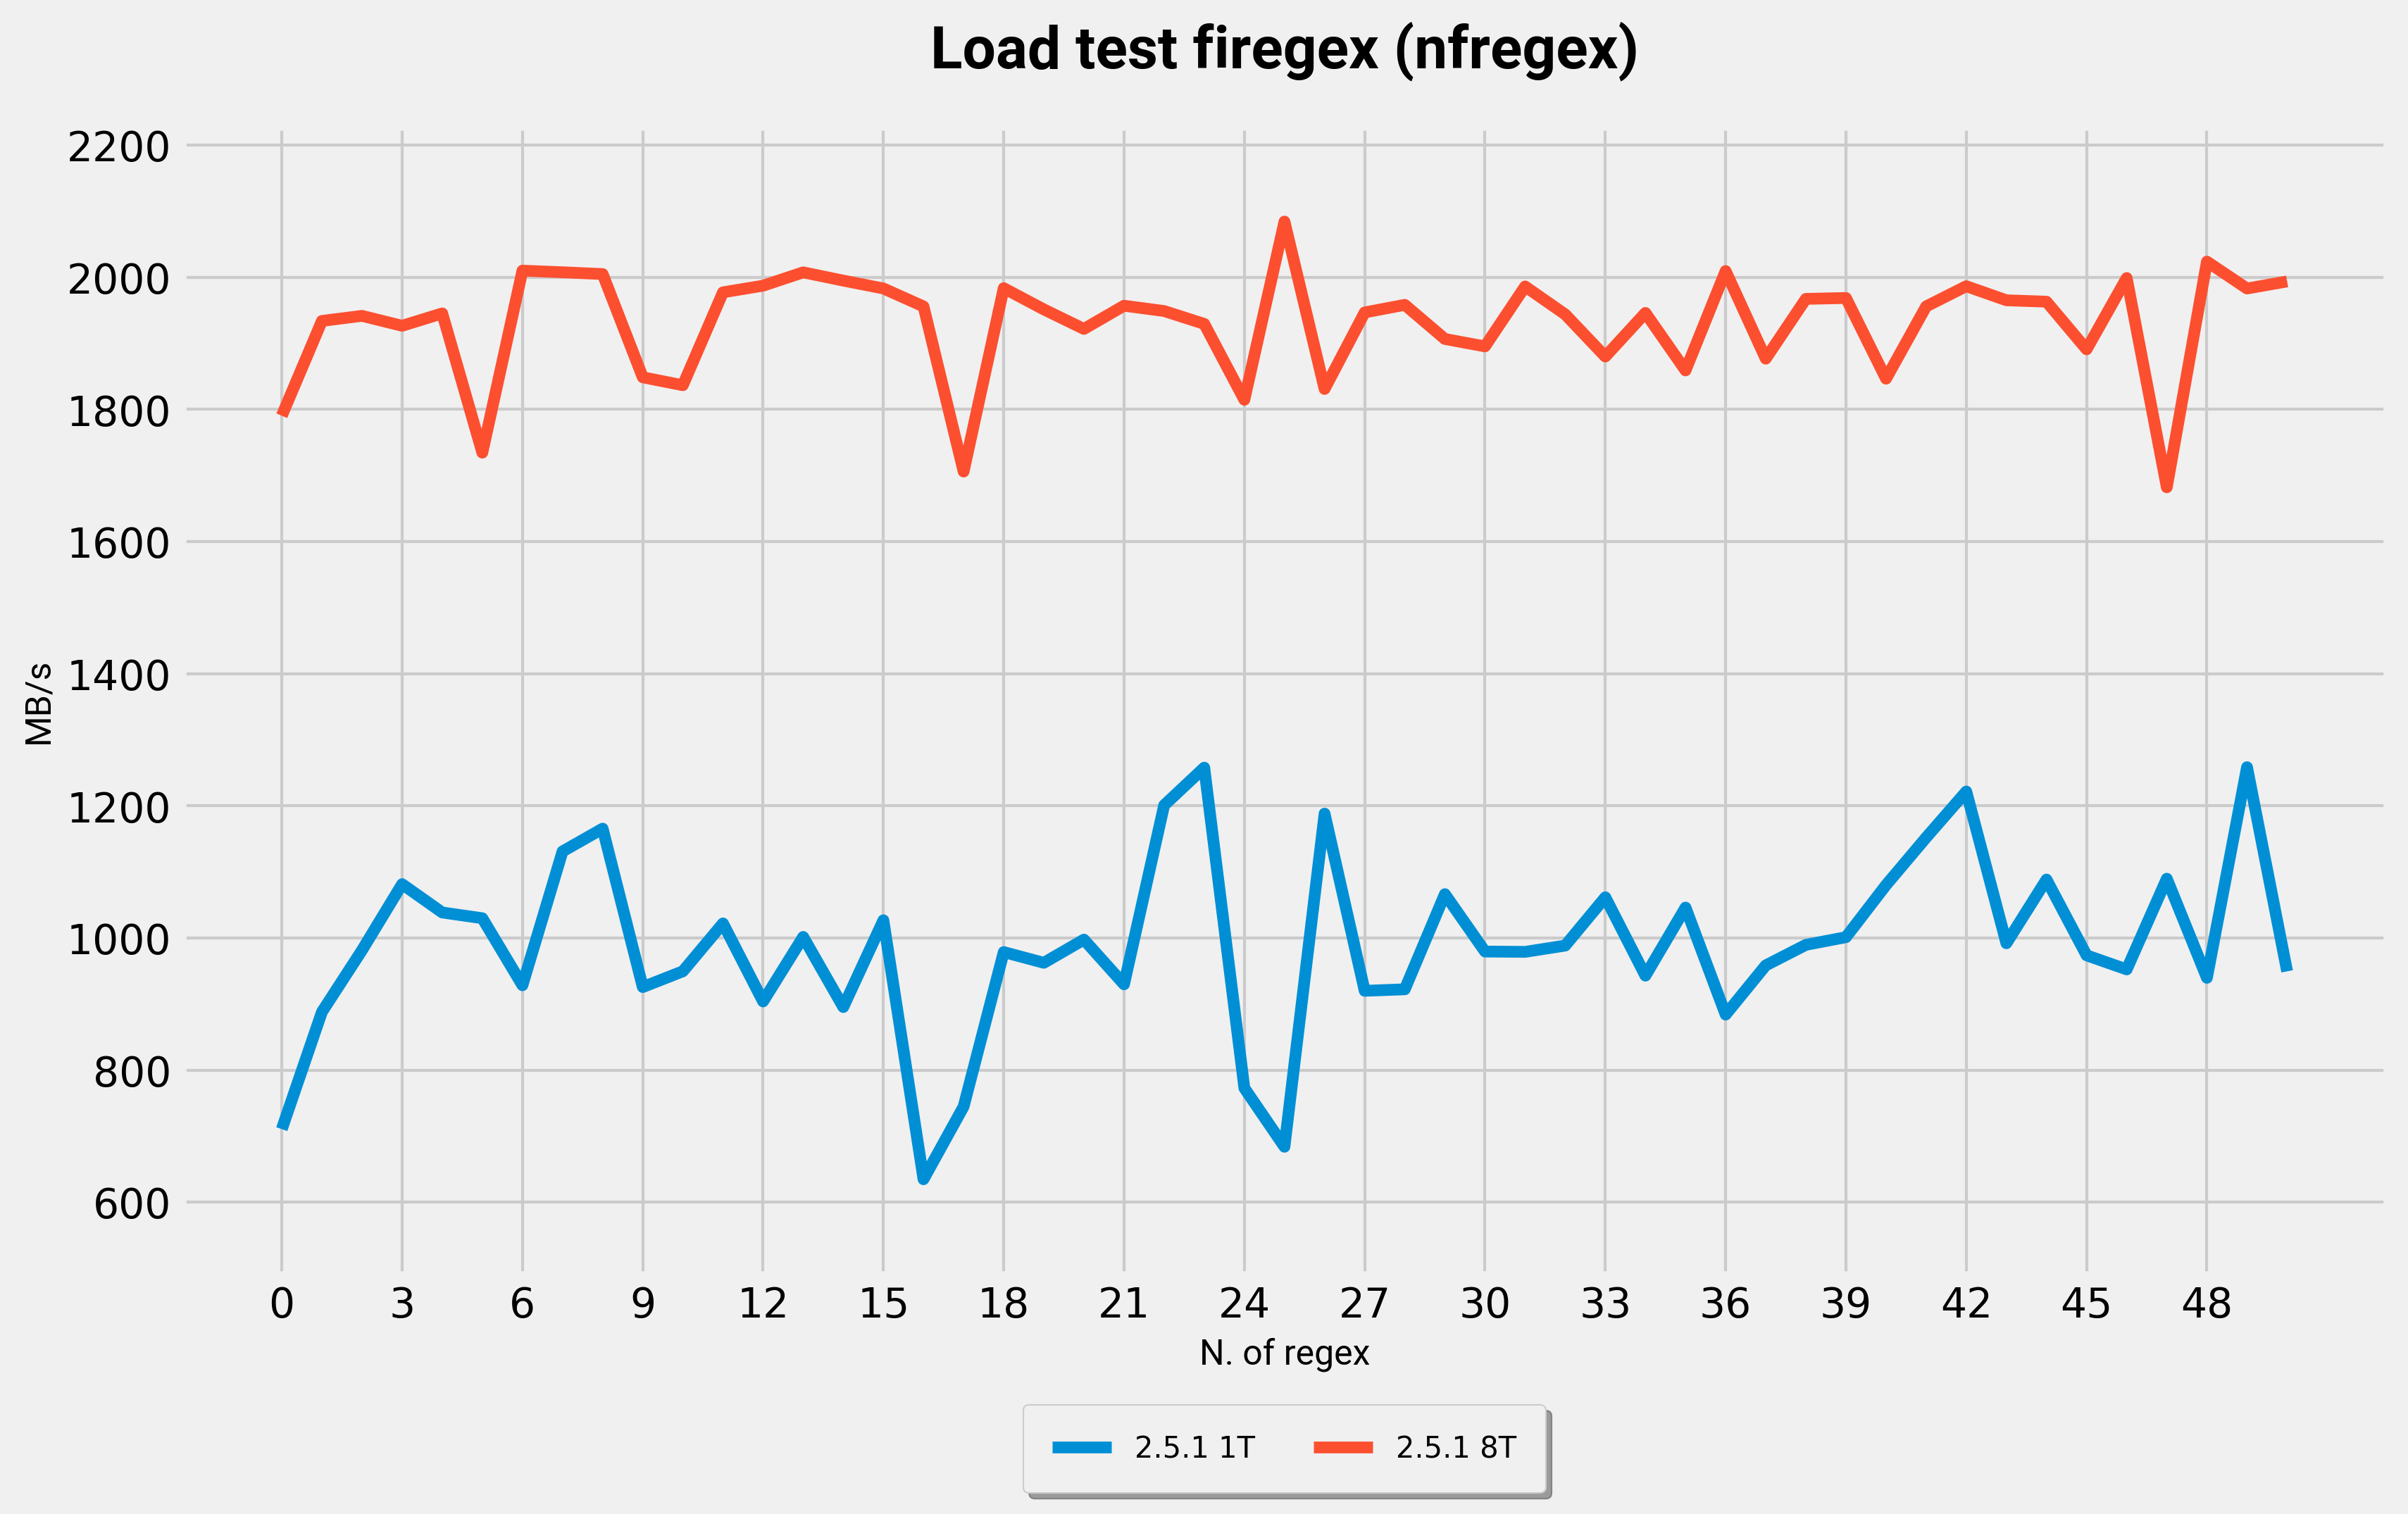
\includegraphics[width=0.98\textwidth]{images/chapter3/Benchmark-chart-with-load.png}
    \caption{Benchmark di \gls{nfproxy} con load balancing personalizzato (1 vs 8 thread)}\label{fig:nfproxy_multithread_benchmark}
\end{figure}

I medesimi vantaggi prestazionali si possono riscontrare in \gls{nfproxy}, che condivide la stessa base di codice per l'implementazione del bilanciamento del carico.

\section{Parsing dei pacchetti L3}

All'arrivo dei pacchetti nella \gls{nfqueue}, viene eseguita un'analisi immediata del protocollo di livello 3 mediante ispezione dei primi
4 bit del campo version, valida sia per IPv4 che \gls{ipv6}. Identificata la versione \gls{ip}, il parsing multilivello viene delegato a
libtins\footcite{\url{https://libtins.github.io/}}{libtins}, che ricostruisce ricorsivamente gli header di rete e trasporto. 

La libreria genera automaticamente lo stream\_id, struttura dati univoca per identificare connessioni TCP/UDP attraverso
una coppia di tuple (\gls{ip}:porta) sorgente/destinazione, che sono ordinate considerano la singola tupla come unica entità, e quindi non slegando mai
\gls{ip} e porta tra loro. Questo approccio permette di identificare univocamente una connessione, indipendentemente dalla direzione del traffico (ingresso/uscita).

\begin{listing}[H]
\begin{minted}[
    frame=single,
    framerule=0.8pt,
    fontsize=\footnotesize,
    breaklines
]{cpp}
PktRequest(const char* payload, size_t plen, T* ctx, mnl_socket* nl, 
           nfgenmsg *nfg, nfqnl_msg_packet_hdr *ph, bool is_input):
    ctx(ctx), nl(nl), res_id(nfg->res_id),
    packet_id(ph->packet_id), is_input(is_input),
    packet(string(payload, plen)),
    action(FilterAction::NOACTION),
    is_ipv6((payload[0] & 0xf0) == 0x60) // Verifica versione IP
{
    if (is_ipv6){
        ipv6 = new Tins::IPv6((uint8_t*)packet.c_str(), plen); // Parsing IPv6
        sid = stream_id::make_identifier(*ipv6); // Generazione stream_id
        _original_size = ipv6->size();
    }else{
        ipv4 = new Tins::IP((uint8_t*)packet.c_str(), plen); // Parsing IPv4
        sid = stream_id::make_identifier(*ipv4); 
        _original_size = ipv4->size();
    }
    l4_proto = fill_l4_info(); // Estrazione info layer 4
}
\end{minted}
\caption{Costruttore di PktRequest e parsing nel pacchetto di rete in firegex}\label{lst:pktrequest_constructor}
\end{listing}

Inoltre lo stream\_id è indipendente dal protocollo internet utilizzato, identificando anche connessioni miste IPv4/IPv6: questo permette di utilizzare la stessa queue per interfaccie di rete differenti, carattertistica potenzialmente utile per implementare nuove feature sulla selezione del traffico da inoltrare alla queue.

Ogni produttore utilizza questo dato come chiave per individurare i dati relativi ad una specifica connessione, salvandoli in una std::map\footcite{\url{https://en.cppreference.com/w/cpp/container/map}}{std_map} diversa per ogni singolo produttore, così implementabile per merito del meccanismo di smistamento dei pacchetti descritto precedentemente.

Il produttore, ricevuto il pacchetto, lo ingloba in un oggetto PktRequest, che contiene tutte le informazioni necessarie per l'elaborazione del pacchetto, e lo inserisce nella coda condivisa del produttore di riferimento.
Sarà il produttore che una volta elaborato il pacchetto ed inviato il verdetto al kernel, deallocherà questa struttura passando all'elaborazione del prossimo pacchetto. Nessuna copia in memoria è pertanto necessaria in questo passaggio.

\section{Gestione dei pacchetti TCP}

Come citato precedentemete, prima di inizializzare la queue, vengono inseriti tramite \gls{nftables} le regole per intercettare il traffico in un certo punto della catena di netfilter, per essere mandato alla queue che determinerà un verdetto sul pacchetto.

\begin{figure}[H]
    \centering
    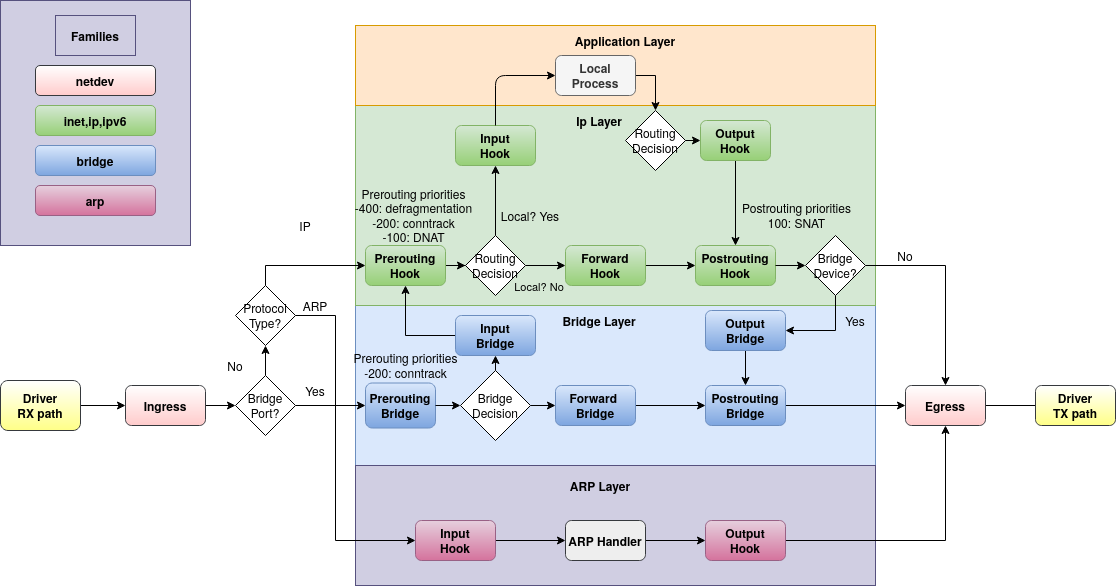
\includegraphics[width=0.98\textwidth]{images/chapter3/nf-hooks.png}
    \caption{Grafico degli hooks di Netfilter Tables}\label{fig:nftables_hooks}
\end{figure}

Il traffico in particolare viene intercettato sia in pre-routing, che in post-routing ad un hook prima dell'azione del modulo conntrack, ma dopo dell'azione di defrag, rispettivamente a prio -310 in pre-routing e 110 in post-routing rientrando nei range corretti, come riportati sulla wiki ufficiale di \gls{nftables}\footcite{\url{https://wiki.nftables.org/wiki-nftables/index.php/Netfilter_hooks}}{netfilter_hooks}. Questo permette di ottenere dei pacchetti che hanno già subito il processo di deframmentazione a livello 3, di cui pertanto non ci dovremo preoccupare, ma che non hanno subito il processo di routing (che quindi volendo potremmo manipolare) e che non sono stati ancora analizzati dal modulo conntrack.
Tuttavia, qui i pacchetti non hanno subito il processo di ordinamento dei payload che avviene a livello 4, sul quale come è possibile osservare dalla Figura~\ref{fig:nftables_hooks}, non è possibile intercettare del traffico, poiché i pacchetti arriveranno direttamente alle fasi di gestioni dei dati per la loro consegna alla socket a livello applicatvo.
Pertanto è dato a noi il compito di analizzare il traffico, ordinando i pacchetti \gls{tcp} per un'utilizzo dei dati coerente a quelli che saranno letti dall'applicazione.
Libtins semplifica significativamente questa gestione attraverso meccanismi automatizzati gestiti dal suo \gls{tcp} follower\footcite{Esempio \gls{tcp} Follower: \url{https://libtins.github.io/examples/http-requests/}}{libtins_tcp_follower_gh} per:  
\begin{itemize}
    \setlength{\itemsep}{2pt}
    \item Chiusura dei flussi \gls{tcp} basata su:
    \begin{itemize}
        \setlength{\itemsep}{1pt}
        \item Analisi del traffico (flag FIN/RST)
        \item Timeout configurabili (rilevamento di inattività)
        \item Utilizzo eccessivo dei buffer di memoria
    \end{itemize}
    \item Ricostruzione dello stream da segmenti non ordinati (o duplicati)
    \item Gestione automatica della memoria utile alla ricostruzione
\end{itemize}
Il follower inoltre permette facilmente l'integrazione di dati gestiti esternamente, tramite il suo sistema di callback, che ne chiamerà le funzionalità compatibilmente con quanto fatto con i buffer internamente.
Le callback permettono di gestire le seguenti operazioni:
\begin{itemize}
    \setlength{\itemsep}{2pt}
    \item Inizializzazione contesti
    \item Pulizia risorse
    \item Propagazione di eventi critici (per chiusure anomale dei flussi)
\end{itemize}

Ogni processo consumatore ha un suo follower dedicato che analizzerà i flussi relativi alla porzione traffico a lui dedicata.

\section{Modifica dei pacchetti}

Il modulo \gls{nfqueue} consente effettivamente la modifica dei pacchetti, offrendo potenzialmente la possibilità di alterare header
\gls{ip}/\gls{tcp} e payload. Tuttavia, questa funzionalità, seppur teoricamente disponibile, è stata implementata solo parzialmente e non risulta pienamente affidabile.

Le limitazioni derivano da problematiche intrinseche legate all’interazione con i meccanismi di livello di trasporto. Ad esempio, modifiche al payload \gls{tcp} durante connessioni attive potrebbero invalidare checksum o causare inconsistenze nei \gls{seq}uence number. La complessità per garantire coerenza in tutti i possibili scenari (come in caso di ritrasmissioni) rende l’implementazione robusta di questa feature particolarmente onerosa. Inoltre, se gestita male, la modifica del payload potrebbe essere soggetta a vulnerabilità di sicurezza. Valutando il rapporto rischio-beneficio, si è optato per comunque rendere disponibile la funzionalità, seppur parzialmente implementata, ma fortemente disincentivata e volutamente resa meno facilmente accessibile.

L’effettiva necessità operativa risulta infatti marginale nella maggior parte degli scenari \gls{ctf}, mentre i potenziali effetti collaterali verrebbero a compromettere uno degli obiettivi principali: la stabilità del servizio.

Di seguito si riporta una descrizione accurata delle problematiche riscontrate e delle soluzioni proposte, o applicate con relativi limiti e valutazioni rischio/beneficio.

Le problematiche sul calcolo dei campi di integrità dei dati non sono trattate, ma considerate già risolte tramite l'utilizzo di libtins, che si occupa durante la serializzazione del pacchetto di ricalcolare questi campi nei vari layer interessati, pertanto non considerata una problematica rilevante.

L'unica operazione aggiuntiva affrontata su questo, è stata la necessità di reinserire il payload del pacchetto nella catena di \gls{pdu} di libtins, poiché (seppur non documentato), il follower del flusso \gls{tcp} internamente separa di fatto il payload dal pacchetto\footcite{Libtins, istruzione per la separazione del payload nel follower (std::move del payload)}{libtins_payload_move_gh}, rendendone necessario il reinserimento per la corretta serializzazione e calcolo di questi campi.

\subsection{Cambio di dimensione del payload}

Come emerge dalle specifiche stesse del protocollo di trasporto \gls{tcp}\footcite{RFC9293, Transmission Control Protocol (TCP)}{rfc9293}, questo tiene traccia dello stato della corretta recezione dei pacchetti tramite un meccanismo di piggybacking che fa utilizzo dei campi numerici \gls{ack} e \gls{seq}.
Nella trasmissione, il \gls{seq} number indica il byte da cui inizia il payload del pacchetto relativamente alla sua posizione nello stream, mentre il campo \gls{ack} della risposta di conferma proveniente dal ricevente, indica fino a che punto il flusso di dati è stato ricevuto correttamente.

Questo meccanismo è fondamentale per il corretto funzionamento del protocollo e per la corretta ricostruzione del flusso originale: di conseguenza la modifica alla dimensione del payload causa inevitabilmente l'incoerenza di questi valori che porteranno a comportamenti inaspettati, non conformi al normale funzionamento del protocollo.

Per risolvere la problematica descritta, è stato implementato un sistema di traduzione bidirezionale dei campi \gls{seq} number e \gls{ack} number.

Questo meccanismo tenta di mantenere la coerenza logica della comunicazione riconvertendo i valori modificati in modo da preservare la corrispondenza tra la dimensione originale dei pacchetti e le aspettative del client (e viceversa del server).
Il kernel e il \gls{tcp} Follower di libtins ricevono così numerazioni coerenti con le alterazioni applicate, mantenendo la sincronizzazione degli stati di connessione.
Il sistema opera in modo simmetrico per entrambe le direzioni del traffico: le modifiche applicate ai pacchetti in uscita vengono compensate da una riconversione inversa per quelli in entrata. L'attivazione avviene automaticamente alla prima modifica di un pacchetto nella sessione \gls{tcp} e rimane attiva per tutta la durata della connessione, garantendo la persistenza del contesto di traduzione.

Questa conversione avviene tramite il calcolo incrementale dell'offset che intercorre tra la dimensione del flusso originale e la dimensione del flusso modificato.

\begin{listing}[H]
\begin{minted}[
    frame=single,
    framerule=0.8pt,
    fontsize=\footnotesize,
    breaklines
]{cpp}
size_t payload_offset = data_size() - _data_original_size;
if (tcp && payload_offset != 0){
    // incremental update of total offset
    if (is_input){
        ack_seq_offset->in += payload_offset;
    }else{
        ack_seq_offset->out += payload_offset;
    }
}
\end{minted}
\caption{Calcolo dell'offset cumulativo nello stream TCP da correggere in modifica}\label{lst:tcp_ack_seq_transl}
\end{listing}
A seguito della modifica, nei prossimi pacchetti vengono compatibilmente ricalcolati gli \gls{ack} e \gls{seq}, su tutto il traffico.
\begin{listing}[H]
\begin{minted}[
    frame=single,
    framerule=0.8pt,
    fontsize=\footnotesize,
    breaklines
]{cpp}
void fix_tcp_ack(){
    // conversion of ack and seq
    if (is_input){
        tcp->seq(tcp->seq() + ack_seq_offset->in);
        tcp->ack_seq(tcp->ack_seq() - ack_seq_offset->out);
    }else{
        tcp->ack_seq(tcp->ack_seq() - ack_seq_offset->in);
        tcp->seq(tcp->seq() + ack_seq_offset->out);
    }
}
\end{minted}
\caption{Algoritmo di traduzione di \gls{ack} e \gls{seq} numbers a seguito di mangle dei pacchetti}\label{lst:tcp_ack_seq_transl_fixing}
\end{listing}
Un'analisi preliminare e dei test preliminari, suggerirebbero l'adeguatezza di questa soluzione. Tuttavia, a seguito di analisi più accurate, si evince come il meccanismo presenti limitazioni intrinseche in determinate casistiche di traffico. L'approccio risulta efficace esclusivamente in condizioni ideali di trasmissione, dove non si verificano fenomeni di ritrasmissione di pacchetti.

La criticità principale risiede nell'algoritmo di conversione, che non considera adeguatamente le ritrasmissioni di segmenti antecedenti al pacchetto modificato. In tali scenari, il ricalcolo dell'\gls{ack} relativo richiederebbe l'utilizzo di un offset compatibile non all'ultimo offset calcolato, ma allo stato del flusso nella parte interessata dalla ritrasmissione, operazione che l'implementazione corrente non esegue. La problematica è diretta conseguenza della mancanza di un analisi del traffico contestuale, capace di identificare la porzione di flusso effettivamente coinvolta nella ritrasmissione, e di memorizzare le discrepanze cumulative associandole direttamente alle varie parti dello stream interessate.
\begin{figure}[H]
    \centering
    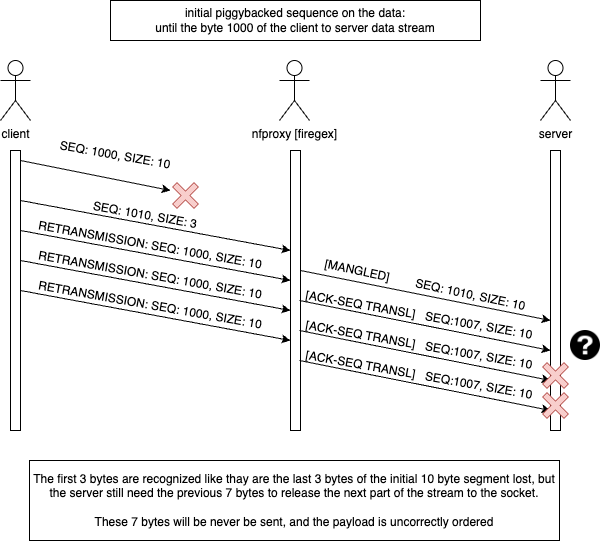
\includegraphics[width=0.90\textwidth]{images/chapter3/TCP_ack_seq_transl_failure.drawio.png}
    \caption{Esempio di una possibile problematica nella traduzione di \gls{ack} e \gls{seq} implementata}\label{fig:tcp_ack_seq_transl_failure}
\end{figure}
L'analisi della Figura~\ref{fig:tcp_ack_seq_transl_failure} evidenzia come le casistiche descritte possano compromettere integralmente il sistema di traduzione implementato. Tali scenari, particolarmente probabili in condizioni di congestione di rete, rappresentano potenziali vettori d'attacco mirati a destabilizzare il servizio.

Alla luce di queste considerazioni, si conclude che la soluzione proposta non possiede la robustezza necessaria per un'implementazione definitiva. La funzionalità di modifica pacchetti viene pertanto mantenuta come opzione sperimentale, accompagnata da avvertenze esplicite sul suo comportamento instabile.

Una soluzione teoricamente più solida richiederebbe la memorizzazione di informazioni aggiuntive riguardo i vari punti del flusso dove il traffico è stato modificato, insieme agli offset applicati in quegli specifici intervalli, per tutta la finestra di trasmissione ancora non riscontrata dal ricevente. Inoltre, sarebbe necessaria una logica di traduzione più complessa per gli \gls{ack}/\gls{seq}, che vada ad esguire un calcolo corerente di questi valori, basato sul posizionamento che il segmento ha in trasmissione o riscontro nel flusso complessivo, sfruttando le nuove informazioni memorizzate.

Considerando il rapporto costo-beneficio e il limitato valore operativo della funzionalità, si è optato per mantenere lo stato corrente dello sviluppo, consapevoli delle possibili criticità che può portare, non essendo una soluzione definitiva.

\subsection{Modifica di segmenti non ordinati}

Un'ulteriore criticità emerge nella gestione dei pacchetti con payload \emph{out-of-order} da modificare. Nell'implementazione corrente, i pacchetti non ordinati vengono analizzati dal \gls{tcp} Follower di libtins per la ricostruzione dello stream ed accettati immediatamente dopo questa elaborazione, privando tuttavia il sistema della possibilità di modificarli successivamente. Questo meccanismo, sebbene un payload malevolo venga accettato, riesce comunque a bloccarlo a livello applicativo, prima che il flusso possa essere completamente riordinato, intervenendo sul pacchetto con la prima parte del payload non ordinato, che normalmente andrebbe a causare il riempimento del buffer del socket a livello applicativo, ma che in questo caso causerà, grazie all'intervento di firegex, un blocco della connessione \gls{tcp}.

Una soluzione alternativa prevedrebbe il buffering dei pacchetti \emph{out-of-order} in attesa dei segmenti mancanti, applicando modifiche retroattive sui pacchetti trattenuti. Tuttavia, questo approccio introdurrebbe: una complessità significativa nel meccanismo di ricostruzione distribuita del flusso e il rischio di saturare la \gls{nfqueue} kernel-side, con conseguente perdita di pacchetti e possibile esposizione ad attacchi DoS mirati a sfruttare le debolezze di questo sistema, potenzialmente portandolo ad un blocco del traffico non desiderato.

Sulla base di queste considerazioni, si conclude che il riscontro immediato dei pacchetti è un approccio che deve essere applicato al fine di scongiurare possibili criticità riguardanti il riempimento della coda kernel, soggetta a questa tipologia di attacchi. La scelta progettuale attuale, seppur limitante, garantisce un'operatività ed un throughput stabile e prevedibile, mantiene il sistema immune a possibili vulnerabilità ma non offre la possibilità di eseguire modifiche su pacchetti non ordinati.

Sarebbe possibile progettare un sistema che eviti i problemi di saturazione della coda kernel, implementando ad esempio un meccanismo basato su dei timeout che evitino la saturazione della coda eliminando i pacchetti potenzialmente fraudolenti. Tuttavia simili implementazioni richiederebbero un'attenta analisi ed uno studio molto più approfondito rispetto a quanto fatto finora, considerando anche un vasto spettro di casistiche insidiose che non si ritiene necessario affrontare in questa tesi e ai fini dello sviluppo di questo modulo.

\section{Parsing dei pacchetti HTTP}

Dall'analisi delle soluzioni esistenti per il parsing di pacchetti \gls{http} è emersa l'assenza di strumenti compatibili con i requisiti specifici del progetto, in particolare per quanto riguarda l'integrazione con le funzionalità introdotte dal \gls{pep} 684\footcite{\url{https://peps.python.org/pep-0684/}}{pep648}. La necessità di supportare l'inizializzazione multi-fase (multi-phase initialization\footcite{\url{https://peps.python.org/pep-0489/}}{pep489}) e garantire thread safety ha reso indispensabile un approccio personalizzato.

La soluzione adottata si basa su un mio fork, che parte dall'implementazione del wrapper python di Derrick Lyndon Pallas\footcite{Python wrapper per llhttp: \url{https://github.com/pallas/pyllhttp}}{original_pyllhttp_impl}, del parser llhttp\footcite{\url{https://github.com/nodejs/llhttp}}{llhttp} sviluppato per Node.js. Questo fork, pubblicamente disponibile su GitHub\footcite{\url{https://github.com/domysh/pyllhttp}}{pyllhttp_fork} e distribuito tramite \gls{pypi}, va a risolvere le limitazioni tecniche derivanti dalla sua versione originale e preserva le capacità core di llhttp, tra cui il parsing zero-copy dei dati, e la validazione rigorosa del protocollo \gls{http}/1.1\footcite{RFC2616, Hypertext Transfer Protocol -- HTTP/1.1}{rfc2616}.

\subsection{Supporto agli algoritmi di compressione in HTTP}

Nel traffico \gls{http} sono spesso in uso algoritmi di compressione per ridurre la dimensione del body. Dato il loro ampio utilizzo, al fine di semplificare l'implementazione di filtri che ne richiederebbero l'analisi del contenuto, si è deciso si supportare la decompressione automatica degli algoritmi supportati dal browser chrome:

\begin{itemize}
    \setlength{\itemsep}{2pt}
    \setlength{\parskip}{2pt}
    \item \textbf{\gls{zstd}}\footcite{RFC1952, GZIP file format specification version 4.3}{rfc1952}: Nativamente supportato in python.
    \item \textbf{brotli}\footcite{RFC7932, Brotli Compressed Data Format}{rfc7932}: supportato tramite un'implementazione eseguita da google\footcite{\url{https://github.com/google/brotli}}{brotli_gh}, che tuttavia non supporta il \gls{pep} 684, per cui anche in questo caso è stato sviluppato un fork compatibile disponibile su github\footcite{\url{https://github.com/domysh/brotli}}{brotli_fork}.
    \item \textbf{\gls{zstd}}\footcite{RFC8478, Zstandard Compression and the application/zstd Media Type}{rfc8478}: supportato tramite un wrapper python sviluppato da Sergey Dryabzhinsky\footcite{\url{https://github.com/sergey-dryabzhinsky/python-zstd}}{zstd_ortiginal_python_wrapper}, che tuttavia, essendo anch'esso non compatibile con il \gls{pep} 684, è stato personalizzato in un ulteriore fork\footcite{\url{https://github.com/domysh/python-zstd}}{zstd_fork}.
    \item \textbf{deflate}\footcite{RFC1951, DEFLATE Compressed Data Format Specification version 1.3}{rfc1951}: Implementabile tramite il modulo zlib, nativamente supportato.
\end{itemize}

L'implementazione è stata scritta seguendo le specifiche definite nell'RFC 2616 il quale definisce la possibilità di compressioni multiple, correttamente supportate nell'implementazione finale.
    
\subsection{Supporto alle websocket}

Nell'implementazione per \gls{http}/1.1 è stato incluso anche il supporto alle websocket\footcite{RFC6455, The WebSocket Protocol}{rfc6455}, tramite l'utilizzo della principale libreria python utilizzata per le decodifica dei Frame, ovvero websockets\footcite{\url{https://websockets.readthedocs.io/en/stable/}}{python_websockets}. Da qui sono state prese le funzionalità di decodifica dei frame, e le funzionalità per il supporto all'estensione permessage-deflate\footcite{RFC7692, Compression Extensions for WebSocket}{rfc7692}, per permetterne la decompressione, utilizzando internamente zlib. La complessità nell'implementazione delle websocket si è concentrata sulla necessità di assemblare il flusso di dati correttamente, dato il mancato supporto nativo al parsing in streaming, come invece supportato su llhttp. Nella fase di upgrading della connessione \gls{http}, vengono riconosciuti i plugin abilitati, e viene automaticamente introdotta la gestione dei websocket che si occupa di decodificare i prossimi dati sulla connessione \gls{tcp}.

In caso di fallimento nel parsing dei frame, i dati vengono resi disponibili per il filtraggio, semplicemente come byte grezzi, stesso meccanismo usato in caso di upgrade ad \gls{http}/2 (non supportato attualmente).

\section{Sintassi e gestione dei filtri python}

I filtri Python per \gls{nfproxy} vengono definiti in file singoli (uno per servizio) contenenti funzioni annotate con il decoratore @pyfilter. Queste funzioni, denominate collettivamente pyfilters, accettano parametri tipizzati che rappresentano i dati estratti dal traffico di rete e restituiscono istruzioni di azione (ACCEPT, REJECT, DROP, chiamati statment) determinando il comportamento finale sul pacchetto.  

L'esempio nel Codice~\ref{lst:curl_filter_example} illustra un filtro che blocca le richieste \gls{http} contenenti la stringa `curl' nell'header User-Agent e impedisce gli upgrade a WebSocket:

\begin{listing}[H]
\begin{minted}[
    frame=single,
    framerule=0.8pt,
    fontsize=\footnotesize,
    breaklines
]{python}
from firegex.nfproxy.models import HttpRequest
from firegex.nfproxy import pyfilter, REJECT

@pyfilter
def curl_filter(r: HttpRequest):
    if r.upgrading_to_ws:
        return REJECT  # Blocca upgrade a WebSocket
    if "curl" in r.user_agent:
        print(f"Tentativo accesso con curl: {r.user_agent}")
        return REJECT  # Blocca client curl
\end{minted}
\caption{Esempio di un filtro python per il modulo \gls{nfproxy}}\label{lst:curl_filter_example}
\end{listing}
Il sistema si appoggia sulla libreria firegex\footcite{\url{https://pypi.org/project/firegex/}}{firegex_pypi}, che fornisce sia i decoratori per la definizione dei filtri, sia i modelli dati per l'annotazione dei parametri. Durante la fase di compilazione, \gls{nfproxy} analizza le signature delle funzioni, sullo stesso principio di validazione tipica di pydantic\footcite{\url{https://docs.pydantic.dev/latest/}}{pydantic}, per determinare automaticamente quali layer di protocollo analizzare (es. \gls{http}, \gls{tcp}), eventalmente quali campi estrarre dal payload, attivando internamente una serie di meccanismi per riuscire a soddisfare le richieste dei filtri.

Se un filtro richiede dati non coerenti tra loro, potrebbe essere elaborato ma mai di fatto eseguito.
L'esecuzione avviene tramite dispatch dinamico: a ogni pacchetto corrispondente ai criteri dichiarati nella signature vengono passati gli oggetti istanziati se disponibili, e ne viene successivamente dato un riscontro sull'azione da eseguire tramite il valore di ritorno. L'assenza di un'istruzione return o il ritorno esplicito di None equivalgono a un'azione ACCEPT implicita.

I filtri continuano ad essere eseguiti fino a che tutti quelli attivi non vengono elaborati, o fino a che uno statment diverso da ACCEPT viene restituito.

Le funzionalità per la modifica del traffico sono accessibili tramite lo statment UNSTABLE\_MANGLE, che si occuperà di elaborare le modifiche eseguite al pacchetto, tramite il model RawPacket. Eventuali modifiche tuttavia non andranno ad influenzare gli altri datahandler che non le riveleranno.

Ulteriori dettagli sull'utilizzo dei models (spesso chiamati anche datahandler) sono disponibili nella documentazione integrata nell'interfaccia di firegex.

\subsection{Gestione dei buffer di memoria}

La gestione di flussi di traffico con payload di grandi dimensioni richiede un'attenzione particolare al consumo di memoria, specialmente in contesti ad alto throughput.\@ \gls{nfproxy} implementa un sistema di bufferring che consente una dimensione massima predefinita di 1MB per ciascun tipo di datahandler, tentando di mantere il corretto funzionamento dei parser anche in condizioni di sovraccarico. Infatti quando la soglia viene superata, il buffer viene automaticamente svuotato sebbene ciò possa comportare perdita di informazioni utili.

Il comportamento predefinito è configurabile attraverso variabili globali che permettono di adattare il bilanciamento tra consumo di risorse e completezza analitica. È possibile ridurre la dimensione massima dei buffer per ambienti memory-constrained o aumentarla per scenari che richiedono la ricostruzione completa di flussi complessi. In aggiunta, l'azione da intraprendere al superamento della capacità del buffer può essere personalizzata tra quattro opzioni: svuotamento controllato (FLUSH), accettazione passiva del traffico successivo (ACCEPT), rifiuto selettivo della connessione (REJECT), o drop dei pacchetti successivi (DROP).

\begin{listing}[H]
\begin{minted}[
    frame=single,
    framerule=0.8pt,
    fontsize=\footnotesize,
    breaklines
]{python}
from firegex.nfproxy import FullStreamAction

FGEX_STREAM_MAX_SIZE = 4096  # Limite dimensionale per tipo di datahandler
FGEX_FULL_STREAM_ACTION = FullStreamAction.REJECT  # Politica di overflow

# Configurazione ottimizzata per flussi medio-piccoli
# Connessioni che superano 4KB vengono chiuse preventivamente
\end{minted}
\caption{Esempio di configurazione di un filtro nfproxy per l'ottimizzazione del consumo di memoria}\label{lst:nfproxy_memory_limit_example}
\end{listing}

\section{Proxy di simulazione}

Per validare il corretto funzionamento dei filtri prima del deployment sul firewall, firegex integra un ambiente di simulazione basato su proxy \gls{tcp}.\@ Questo strumento, accessibile tramite il comando fgex \gls{nfproxy}, consente di testare le regole in condizioni controllate riproducendo fedelmente l'architettura operativa del modulo reale.
\begin{listing}[H]
\begin{minted}[
    frame=single,
    framerule=0.8pt,
    fontsize=\footnotesize,
    breaklines
]{bash}
fgex nfproxy test_http.py domy.sh 80 --proto http
\end{minted}
\caption{Comando per avviare il simulazione di nfproxy integrato nella \gls{cli} di firegex}\label{lst:nfproxy_sim_cmd}
\end{listing}

Questo comando avvia un proxy sull'indirizzo specificato (in questo caso domy.sh:80) applicando i filtri definiti in test\_http.py.
Per verificare gli effetti che i filtri avrebbero sul nostro server, possiamo configurare il simulatore per inoltrare il traffico al nostro server reale, interagendoci però tramite la connessione aperta dal simulatore stesso. In questo modo possiamo testare l'effettiva applicazione delle regole senza compromettere il funzionamento del server nella rete di gara.

Inoltre il simulatore supporta l'hot-reload dei filtri, rilevando automaticamente le modifiche ai file Python senza richiedere riavvii. Questo sistema permette di testare rapidamente le modifiche ai filtri, riducendo il tempo di sviluppo e semplificando il processo di debugging.

Si specifica che il simulatore si occupa unicamente di replicare a grandi linee il comportamento della parte c++ del modulo, ma utilizza esattamente lo stesso codice per eseguire il parsing e per l'esecuzione dei filtri, permettendo nella maggior parte dei casi di avere un comportamento pressochè identico a quello che si avrebbe in produzione.

La Figura~\ref{fig:nfproxy_sim} illustra l'output del simulatore durante l'esecuzione di un filtro \gls{http}, mostrando anche l'auto-reload eseguito in seguito all'esecuzione di modifiche.

\begin{figure}[H]
    \centering
    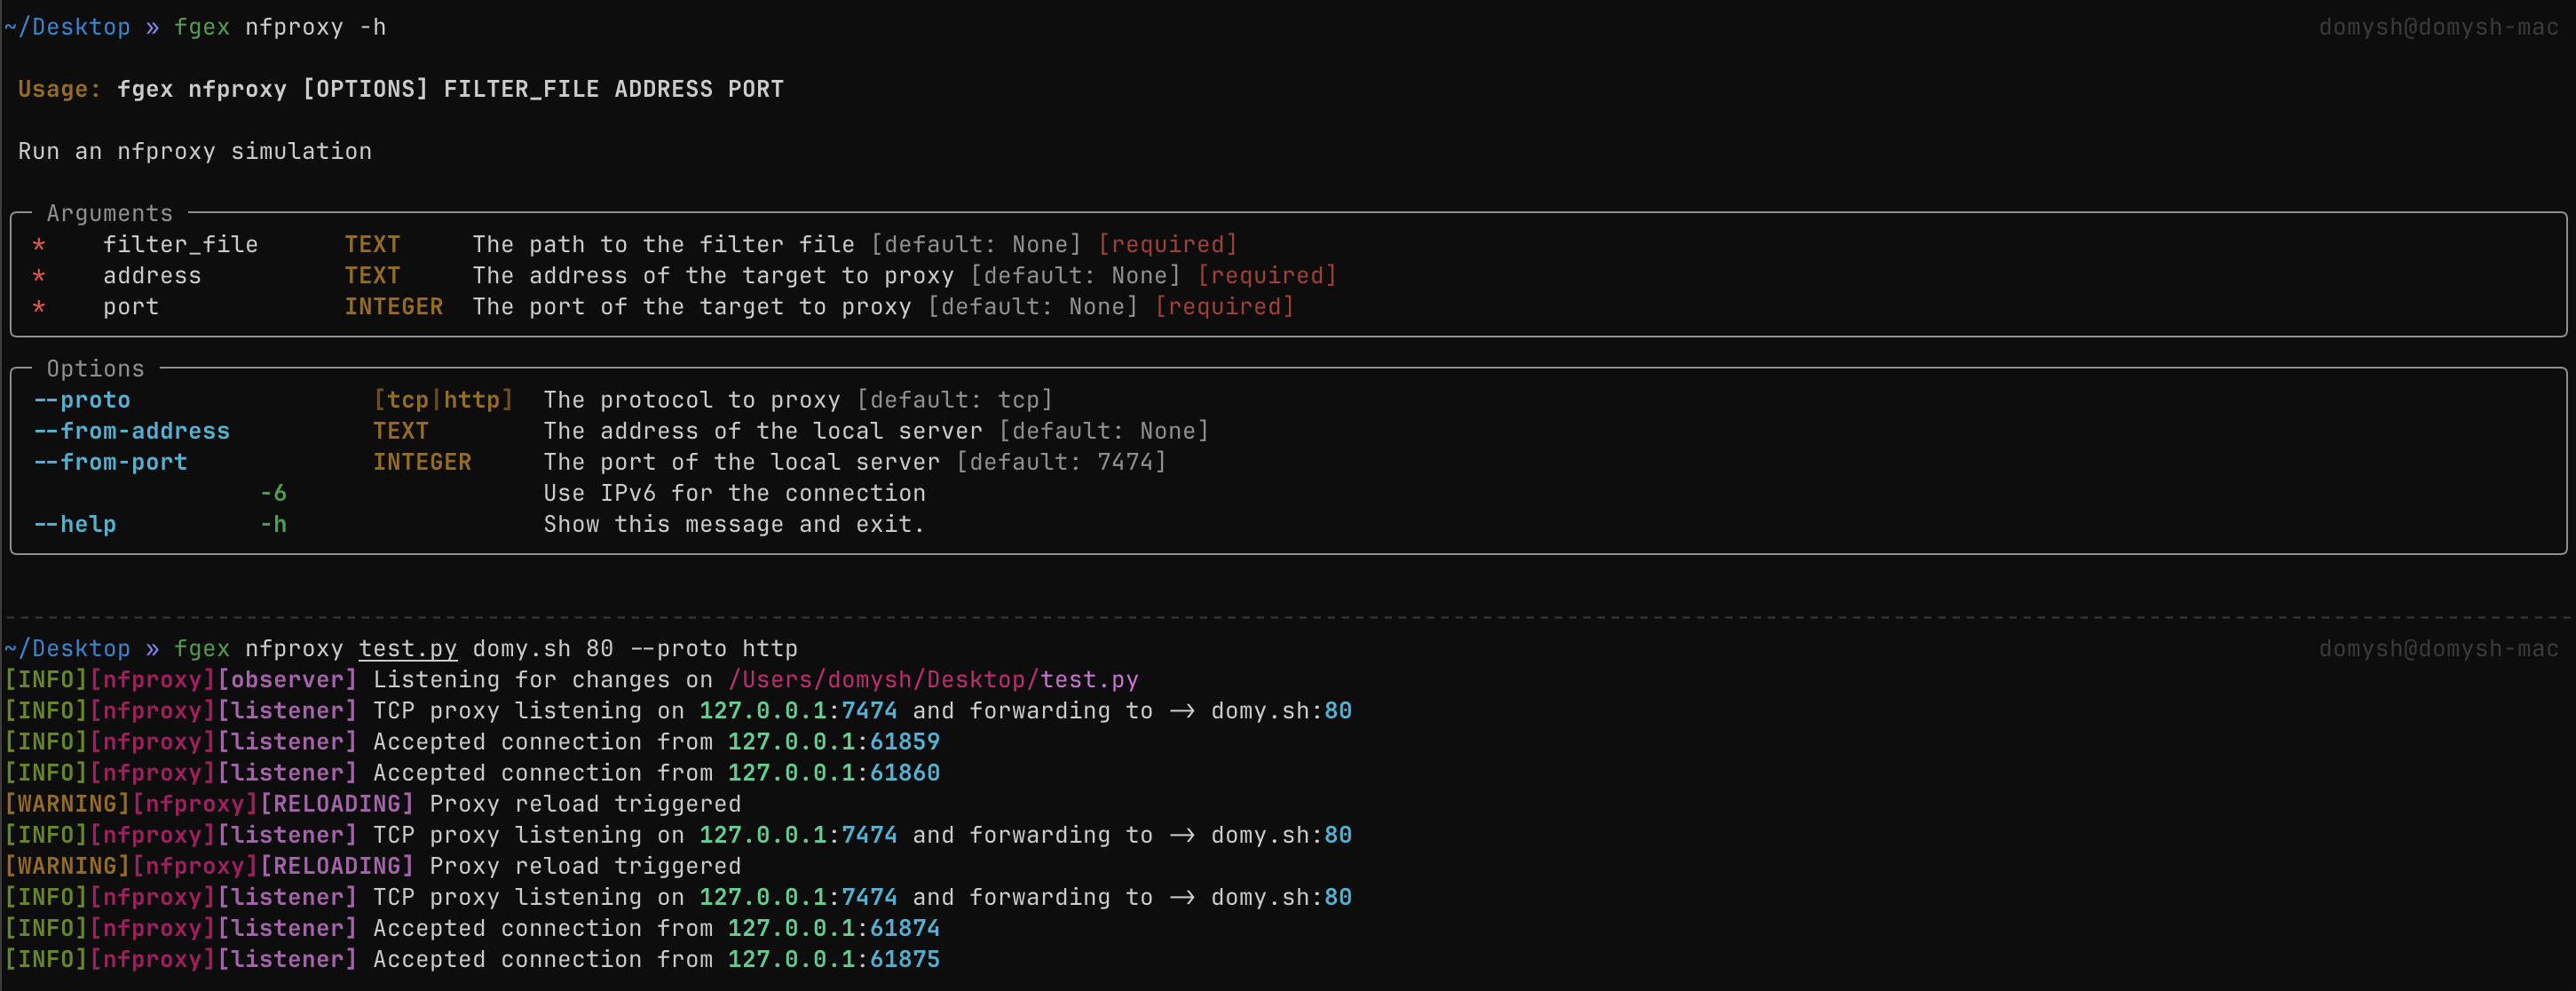
\includegraphics[width=0.98\textwidth]{images/chapter3/nfproxy_sim.png}
    \caption{Simulazione di \gls{nfproxy} tramite il comando fgex}\label{fig:nfproxy_sim}
\end{figure}


\chapter{Testing e Benchmarking}

Ai fini di verificare il corretto funzionamento del sistema e valutarne le prestazioni, sono stati sviluppati test e benchmark.
Firegex già presentava un set di tests, che con l'integrazione di nfproxy sono stati ampliati e migliorati, al fine di coprire anche le nuove
feature introdotte.\\
I test sono eseguiti prima di ogni rilascio in automatico, al fine di garantire che le modifiche apportate non abbiano introdotto regressioni.
I rilasci di firegex avvengono tramite GitHub Actions, che ad ogni rilascio su GitHub esegue i test e, in caso di successo,
pubblica il container di firegex sul Github Container Registry (ghcr.io/pwnzer0tt1/firegex) e rilascia una nuova versione della libreria inclusa 
nello stesso repository su PyPi.\\
I rilasci avvengono sia per architetture \texttt{x86\_64} che \texttt{ARM64}, al fine di supportare il maggior numero di dispositivi possibile.\\

\section{Integrazione dei test}

I test sono stati integrati nel repository di firegex, all'interno della cartella \texttt{tests}.\\
I test riguardanti nfproxy sono contenuti nel file \texttt{tests/nfproxy\_test.py}, ed esegue la seguente serie di operazioni:

\begin{itemize}
    \setlength{\itemsep}{5pt}
    \setlength{\parskip}{5pt}
    \item Avvia un nuovo servizio sull'interfaccia di loopback, e verifica che il traffico non sia stato compromesso dal semplice avvio del modulo.
    \item Verifica che ogni tipo di vedict stia correttamente funzionando inserendo un filtro che verifica se sul segmento TCP sia presente un payload specifico.
    Verificando che il traffico si comporti coerentemente al fatto che il payload specifico sia stato scambiato o meno.
    \item Si verifica che il verdict di UNSTABLE\_MANGLE funzioni correttamente, testando sia mangle a pacchetti più piccoli che più grandi, comprovando
    pertanto che la traduzione degli ack e seq avvenga correttamente generando altro traffico a seguito della modifica.
    \item Si asssucura che le funzionalità di interruzione del servizio e del singolo pyfilter sia correttamente funzionante.
    \item Per ogni tipo di datahandler, si scambiano dei payload di prova al fine di verificare se il parsing dei vari dati avvenga correttamente.
    Datahandler testati: \texttt{TCPInputStream}, \texttt{TCPOutputStream}, \texttt{HttpRequest}, \texttt{HttpResponse}, \texttt{HttpRequestHeader},
    \texttt{HttpResponseHeader} includendo anche il parsing di \texttt{Frame websocket}.
    \item Vengono testate tutte le API backend di nfproxy, verificando che le chiamate restituiscano i valori corretti, e si comportino in modo coerente alla loro funzione.
    \item Si verifica inoltre che vengano contate correttamente le connessioni bloccate, e i pacchetti modificati nelle statistiche.
\end{itemize}

\section{Benchmark}

I benchmark sono stati realizzati tramite uno script python con l'ausilio di \texttt{iperf3}\footcite{\url{https://iperf.fr/}}{iperf_website}.\\
Le casistiche utilizzate sono di semplice natura, verificano le prestazioni in termini di throughput, e lo fanno sia a servizio attivo senza filtri, che con
un filtro che applica la seguente regex al payload TCP (regex per il matching di email):
\begin{verbatim}
    (?:[a-z0-9!#$%&'*+/=?^_`{|}~-]+
       (?:\.[a-z0-9!#$%&'*+/=?^_`{|}~-]+)* |
       "(?:[\x01-\x08\x0b\x0c\x0e-\x1f\x21\x23-\x5b\x5d-\x7f] |
           \\[\x01-\x09\x0b\x0c\x0e-\x7f])*")
    @
    (?:(?:[a-z0-9](?:[a-z0-9-]*[a-z0-9])?\.)+
        [a-z0-9](?:[a-z0-9-]*[a-z0-9])? |
       \[(?:(?:25[0-5] | 2[0-4][0-9] | [01]?[0-9][0-9]?)\.){3}
           (?:25[0-5] | 2[0-4][0-9] | [01]?[0-9][0-9]? |
               [a-z0-9-]*[a-z0-9]:
               (?:[\x01-\x08\x0b\x0c\x0e-\x1f\x21-\x5a\x53-\x7f] |
                   \\[\x01-\x09\x0b\x0c\x0e-\x7f])+)\])
\end{verbatim}

Si da per assodato che i filtri siano correttamente funzionanti (la cui caratteristiche è verificata dai test), e si vuole verificare l'overhead causato
dai filtri che comunque vengono eseguiti e che quindi diminuiscono il throughput.\\
I benchmark sono stati eseguiti su una macchina con le seguenti caratteristiche:\\

\texttt{Macbook Air M2 16GB RAM}\\
\texttt{Su una VM avviata da OrbStack con Fedora Linux 41 (Container Image) aarch64}\\
\texttt{Linux 6.12.13-orbstack-00304-gede1cf3337c4}\\

Lo script python creato è creato appositamente per ripetere la stessa misura un numero variabile di volte, sia sul modulo nfproxy, che sul modulo nfregex.
I risultati sono stati raccolti e analizzati, e messi a disposizioni nei grafici seguenti.\\
I benchmark sono stati eseguiti con i seguenti parametri: \texttt{python3 comparemark.py nfproxy -p testpassword -d 1 -s 50 -V 100} e \texttt{python3 comparemark.py nfregex -p testpassword -d 1 -s 50 -V 100}
con 1 secondo di durata del singolo benchmark, 50 connessioni simultanee, e 100 misure eseguite.\\
Il numero indicato dopo la \texttt{T} nei grafici indica il numero di thread con cui firegex è stato configurato: quindi eseguiti sia in
single-threading che in multi-threading (con 8 thread).\\

\begin{figure}[H]
    \centering
    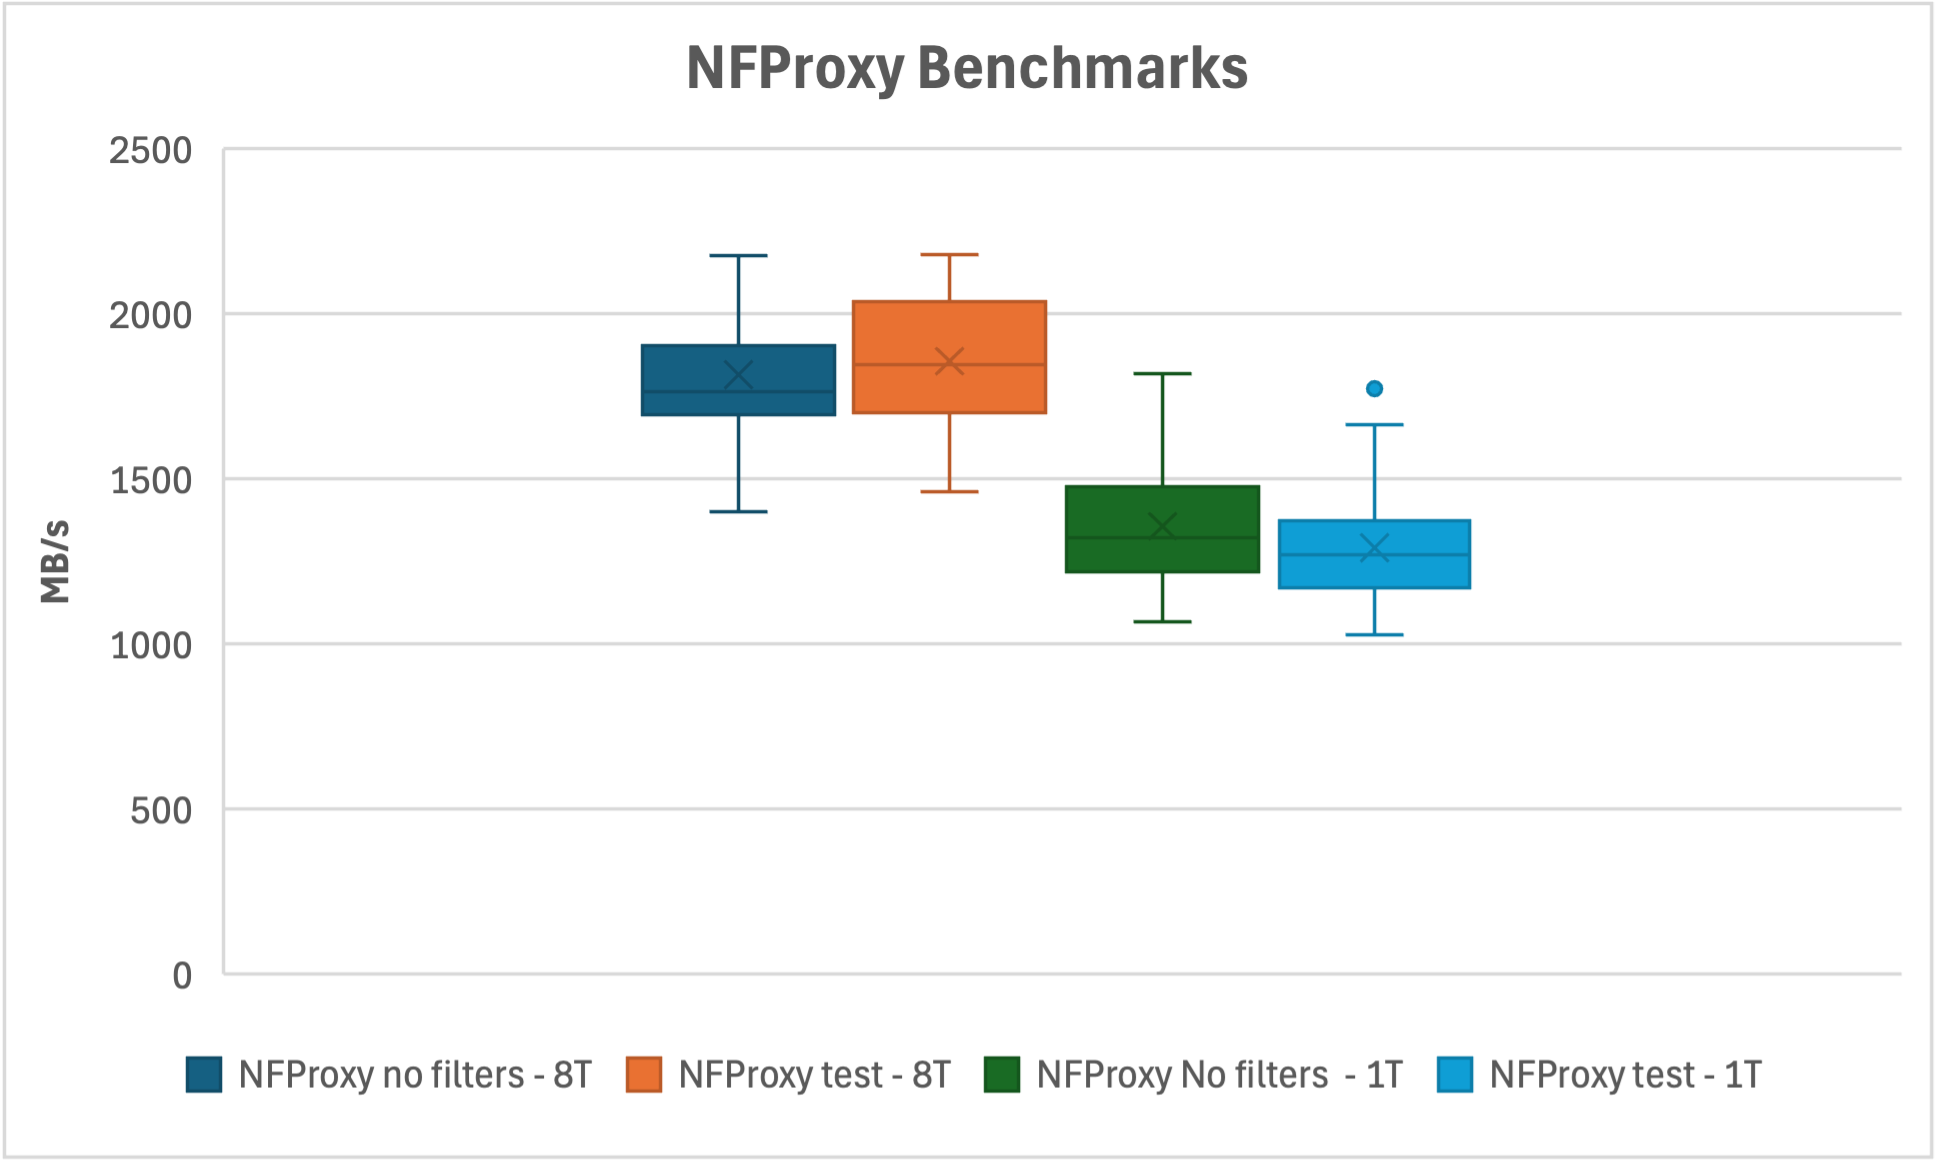
\includegraphics[width=0.98\textwidth]{images/chapter4/whisker_nfproxy.png}
    \caption{Grafico Whisker sulle misure di throughput di nfproxy}\label{fig:wisker_nfproxy}
\end{figure}

\begin{figure}[H]
    \centering
    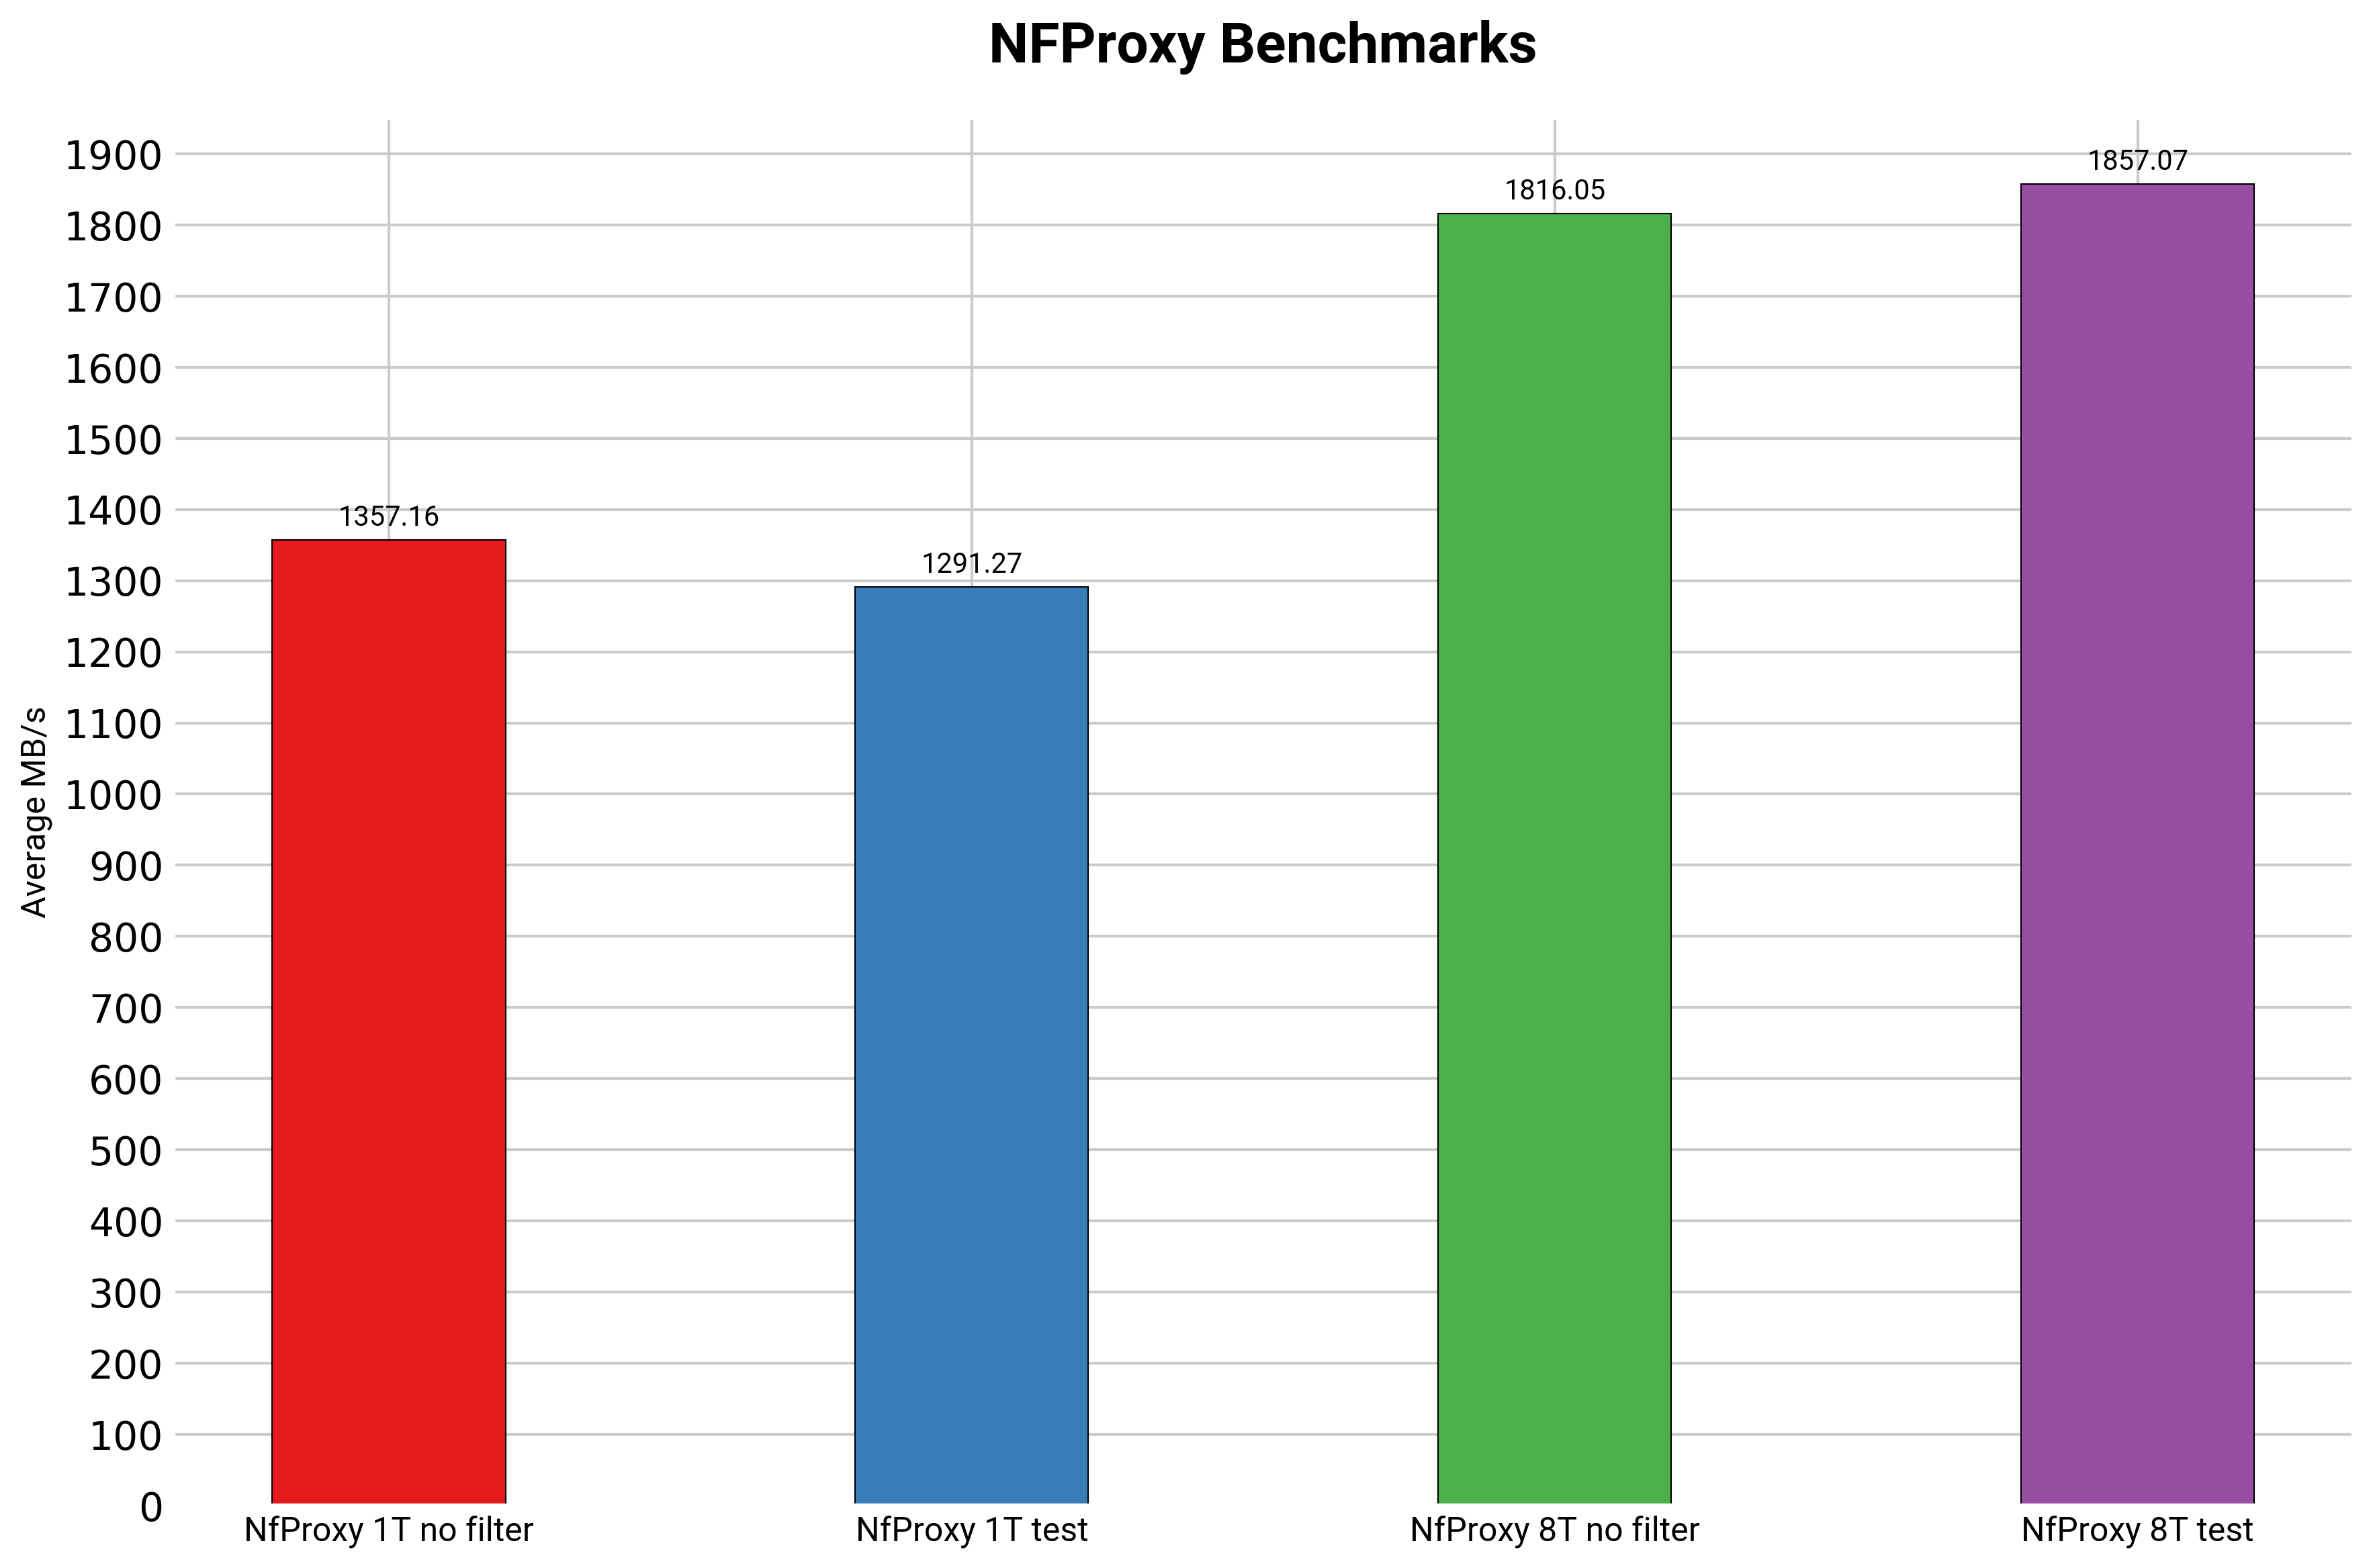
\includegraphics[width=0.98\textwidth]{images/chapter4/istogramma_nfproxy.png}
    \caption{Istogramma sulle misure medie di throughput di nfproxy}\label{fig:istogramma_nfproxy}
\end{figure}

Si può notare come le performance in multi-threading di nfproxy siano migliori rispetto all'utilizzo del singolo thread.

\begin{figure}[H]
    \centering
    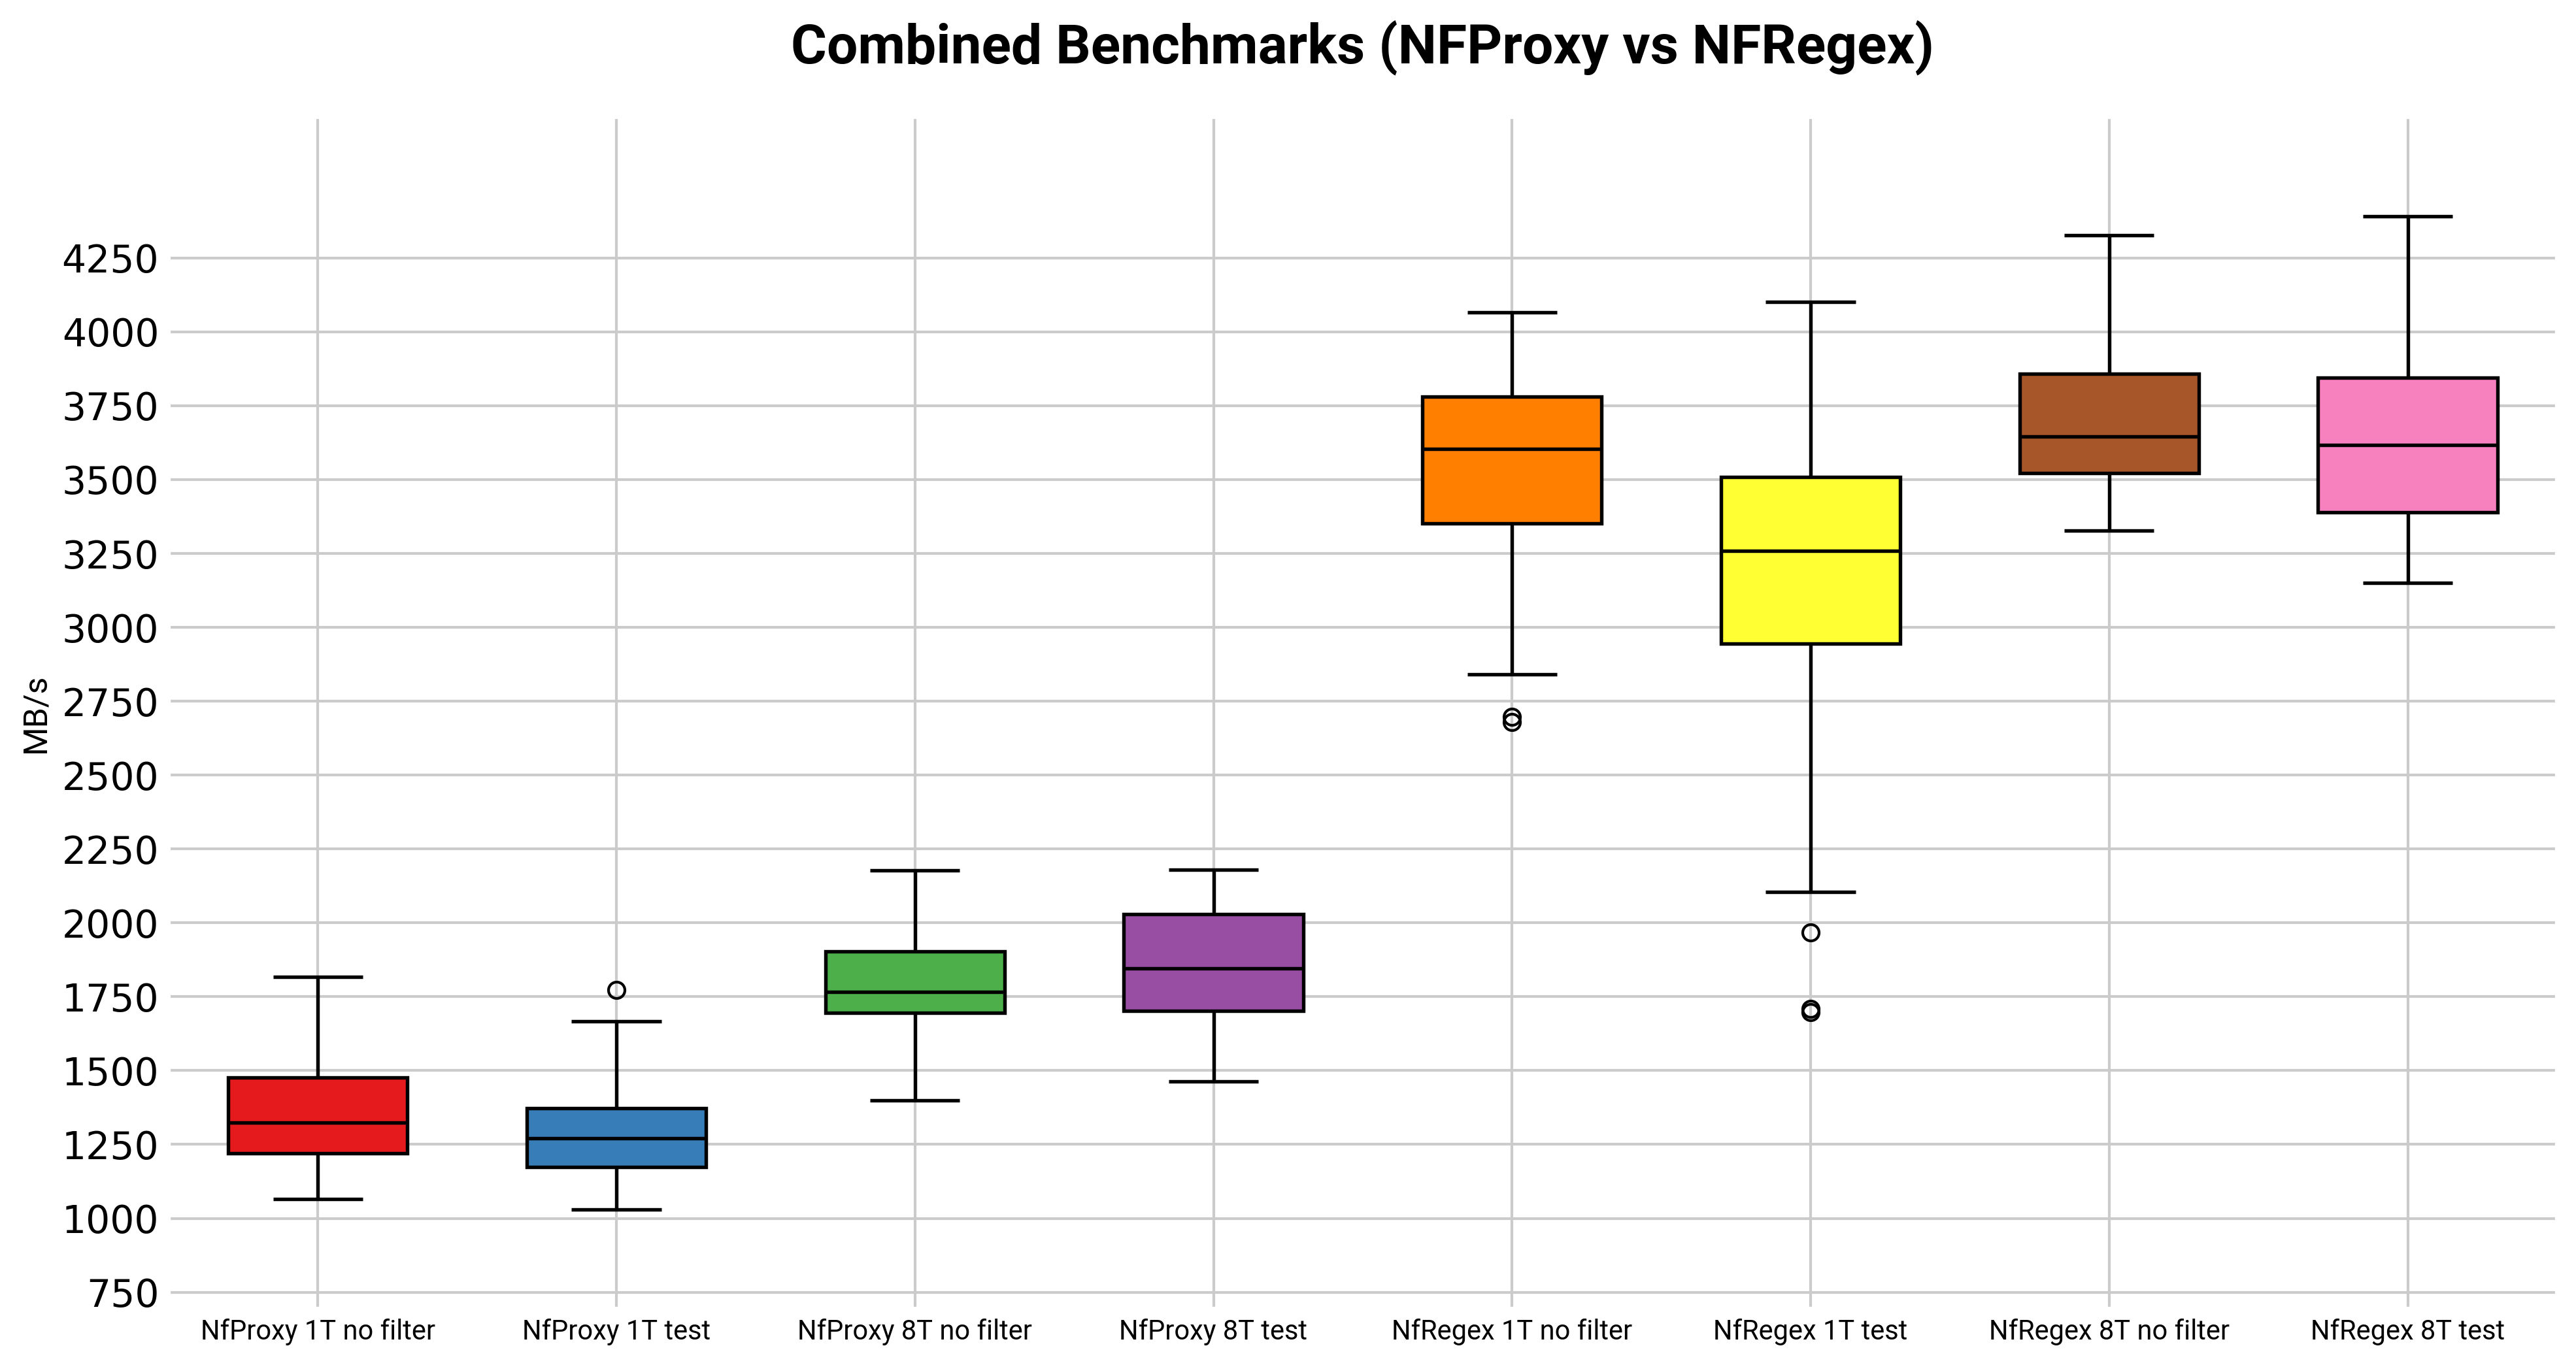
\includegraphics[width=0.98\textwidth]{images/chapter4/whisker_compare.png}
    \caption{Grafico Whisker sulle misure di throughput di nfproxy e nfregex}\label{fig:wisker_nfproxy_nfregex}
\end{figure}

\begin{figure}[H]
    \centering
    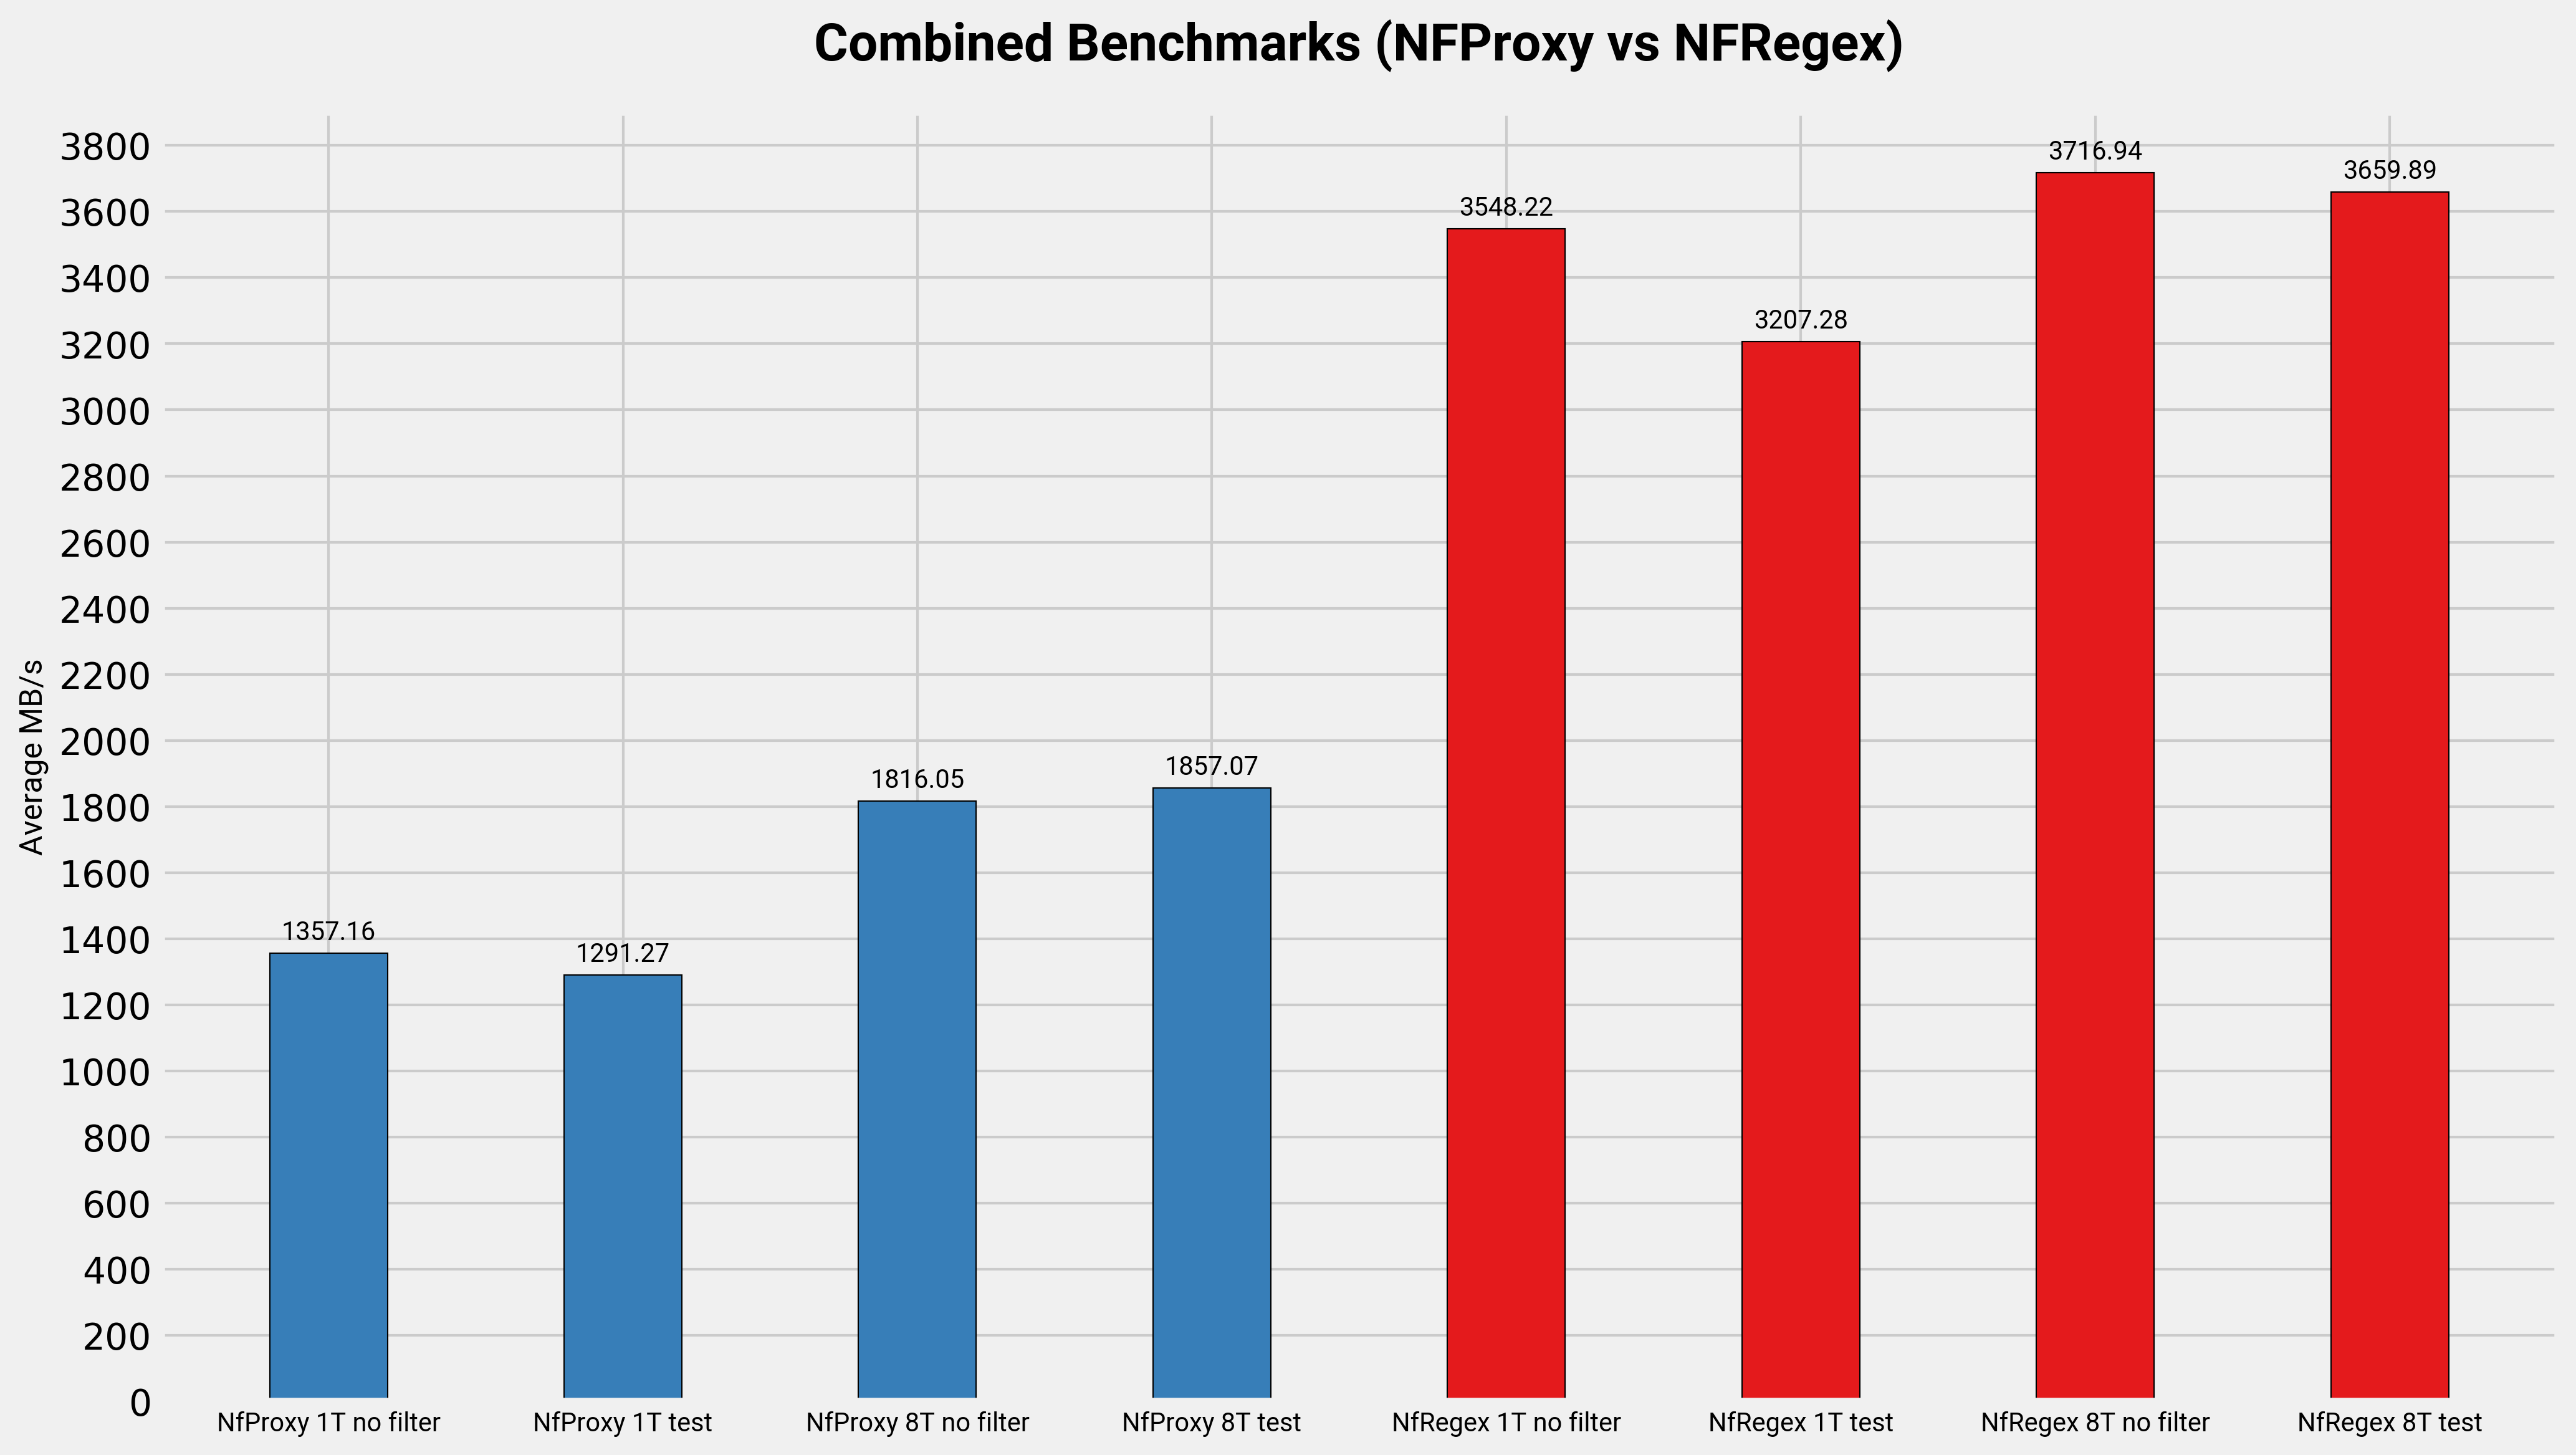
\includegraphics[width=0.98\textwidth]{images/chapter4/istrogramma_compare.png}
    \caption{Istogramma sulle misure medie di throughput di nfproxy e nfregex}\label{fig:istogramma_nfproxy_nfregex}
\end{figure}

Dal confronto di nfproxy e nfregex si può notare come nfproxy abbia un calo di prestazioni rilevante rispetto a nfregex, che tuttavia
rimane comunque abbondantemente alto per supportare anche carichi di rete molto elevati.\\

\chapter{Note e sviluppi futuri}

\section{CVE-2022-36946}

Durante lo sviluppo di \texttt{nfregex} di firegex, è stata scoperta una vulnerabilità di sicurezza che permetteva ad un utente malintenzionato di
causare un crash del kernel.\\
La vulnerabilità è stata prima segnalata al team di sicurezza del kernel e rapidamente risolta nel commit
\url{https://web.git.kernel.org/pub/scm/linux/kernel/git/torvalds/linux.git/commit/?id=99a63d36cb3ed5ca3aa6fcb64cffbeaf3b0fb164}.\\
La vulnerabilità è stata successivamente segnalata a MITRE, nominata come \texttt{CVE-2022-36946}\footcite{\url{https://nvd.nist.gov/vuln/detail/cve-2022-36946}}{cve_2022_36946}.\\

In un primo momento la vulnerabilità ci è sembrata di difficile sfruttamento, in quanto (pensavamo) richiedeva comunque privilegi di amministratore 
o firewall costruiti con funzionalità sfruttabili difficilmente immaginabili da scrivere in contesti reali.\\
Tuttavia, la vulnerabilità è stata classificata come critica, in quanto con l'utilizzo dei linux namespace permette il crash del kernel anche da
un utente non privilegiato.\\

È possibile verificare la vulnerabilità tramite il seguente one-command realizzato da noi: \texttt{curl -sLf https://pwnzer0tt1.it/cve-2022-36946.sh | bash}.\\
Informazioni aggiuntive sono disponibili sulla pagina da noi creata \url{https://github.com/Pwnzer0tt1/CVE-2022-36946}.\\

\section{Sviluppi futuri}

Di seguito si elencano alcuni sviluppi futuri che potrebbero essere implementati per migliorare il modulo nfproxy:

\begin{itemize}
    \setlength{\itemsep}{5pt}
    \setlength{\parskip}{5pt}
    \item \texttt{Implementazione di HTTP/2}: supporto al protocollo HTTP/2 permettendo di codificare tutte le versioni del protocollo su TCP in maniera
    quanto più trasparente nell'utilizzo dei datahandler http.
    \item \texttt{Supporto a UDP}: supporto al protocollo UDP, permettendo di filtrare e modificare i pacchetti UDP. Questione complessa da affrontare
    in questo contesto è la mancanza di un meccanismo per il quale decidere se una determinata connessione è terminata o meno a livello di gestione di memoria.
    \item \texttt{Reimplementazione tramite lo sviluppo di un MITM proxy con address e port translation personalizzato}: permettere di utilizzare gli stessi filtri di nfproxy
    ma realizzando l'impementazione tramite un proxy MITM, che tuttavia non richieda cambi di configurazione sui servizi: ciò sarebbe differente dal
    modulo \texttt{porthijack} poichè il proxy sarebbe gestito da firegex stesso, e si dovrebbe implementare un meccanismo di address e port translation
    ulteriore per cui al server la richiesta sembri provenire all'indirizzo originale.
    \item \texttt{Sviluppo di un modulo per la condivisione di dati tra i vari thread}: permettere di condividere dati tra i vari thread, tramite una struttura apposita in nfproxy
    che con la realizzazione di un modulo python personalizzato in c, permetterebbe di condividere dati tra i vari thread con GIL separati in maniera sicura.
    \item \texttt{Supporto al monitoring delle queue}: permettere di monitorare le queue di netfilter nel frontend di firegex per permettere di comprendere
    meglio il carico associato in real-time sul firewall. Ciò sarebbe possibile tramite le API kernel esposte in \path{/proc/net/netfilter/nfnetlink_queue}.
\end{itemize}

\chapter*{Conclusioni}
\addcontentsline{toc}{chapter}{Conclusioni}

In questo lavoro di tesi si è concluso con successo lo sviluppo del modulo nfproxy per firegex, che permette rispetto ai moduli già esistenti di filtrare con un'elevata flessibilità e accuratezza il traffico, tramite l'implementazione di filtri in linguaggio python.\\

Nonostante il calo di performance, notoriamente previsto, rispetto al modulo nfregex, nfproxy si è dimostrato più che sufficientemente performante per poter essere utilizzato in una competizione Attack-Defense, per merito degli sforzi eseguiti nella progettazione e nell'implementazione
dell'architettura, che ha pernmesso di ottenere ottimi risultati, portandolo a diventare un'ottimo strumento per la difesa dei servizi.\\

Il lavoro fatto per questa tesi può essere inoltre un ottimo punto di partenza per eseguire ulteriori potenziamenti al modulo stesso, ma anche per lo sviluppo di alternative che fanno uso dello stesso modello architetturale qui presentato.\\

Inoltre lo sviluppo di nuove funzionalità, come quelle citate nelle note degli sviluppi futuri, renderebbe nfproxy un modulo ancora più versatile e flessibile di quanto non lo sia già, permettendone l' utilizzo in contesti ancora più ampi e diversificati.\\


\chapter*{Ringraziamenti}
\addcontentsline{toc}{chapter}{Ringraziamenti}

Ringrazio innanzitutto il mio relatore, il Prof. Gennaro Boggia, per avermi supportato durante l'analisi di diverse
problematiche nate durante lo sviluppo stesso del nuovo modulo del firewall. Ringrazio anche il mio correlatore, il Dott. Ing. Daniele Pugliese,
per avermi supportato durante la stesura di questa tesi e per avermi fornito consigli e suggerimenti utili per il completamento
di questo lavoro.\\
Ringraziamento dovuto va alla mia famiglia: a mia madre a mio padre e a mio fratello, per avermi supportato durante tutto il percorso di studi,
per avermi permesso di concentrarmi sul mio percorso di studi e per avermi supportato in ogni momento.\\
Un grande grazie va anche ai tutti i miei amici:\\
A Vanny, per essermi stato vicino non solo durante il percorso di studi, ma anche durante tutto il mio percorso di vita fino ad ora, per l'entusiasmo
per la vita stessa, per i viaggi fatti assieme, per le risate ma sopratuttto per i consigli e i momenti di riflessione e di sfogo in cui
mi, ma sopratutto ci, siamo supportati e rafforzati a vicenda.\\
A Federica, per avermi rialzato nei momenti più bui, sopportandomi e supportandomi in ogni momento, con un affetto e vicinanza imparagonabile e gratuita,
di vitale importanza e di cui te ne sarò sempre grato. Grazie per ogni momento passato assieme nei quali ci siamo distaccati dai problemi, e ci siamo
dedicati a noi stessi e a passare dei momenti di tranquillità e di senerità, dove ogni argomento è ammesso.\\
Ai miei colleghi di studio, Vito e Daniele, per avermi dimostrato un supporto che va oltre il semplice studio a rapporto di colleghi, ma che si concretizza in un
legame fortissimo che si è sviluppato nel corso di questi anni che ha permesso di rendere anche le lezioni più dure da affrontare, più leggere.\\
A Nicola (Guerrera), per tutto il supporto affettivo che mi hai dato, oltre che per supporto nelle idee nei progetti che abbiamo sviluppato assieme,
come quello presentato in questa tesi stessa.\\
A Gilberto, che seppur essendoci conosciuti da relativamente poco tempo, mi hai spesso dimostrato una vicinanza a $2\pi rad$ di supporto ma anche di affetto.\\
A Gianmarco, per avermi sopportato ogni mattina per andare a lezione, e per tutte le sessioni di studio passate assieme per la preparazione degli esami.\\
Ma un grazie va anche a Brian, Claudio, Domenico, Fabio, Francesco, Gerardo, Gianfranco, Lara, Oronzo e Vito: ogniuno di voi ha contribuito a rendere
questo percorso di studi più leggero e più piacevole, per ogni piccolo momento passato assieme, per ogni risata, per ogni momento in cui
mi avete zittito per fermare il mio irrefrenabile bisogno di parlare di informatica.\\

Non scriverò altre parole, ma spero che quelle già scritte siano sufficientemente profonde a dimostrarvi la reale gratitudine che provo nei vostri confronti.\\

Grazie!\\
\begin{flushright}
    \textit{Domingo Dirutigliano}
\end{flushright}


\bibliographystyle{unsrt}  
\bibliography{bibliografia}
\end{document}
